\documentclass[a4paper,12pt]{report}

\usepackage[english]{babel}
\selectlanguage{english}

\usepackage{csquotes}
\usepackage{graphicx} % Pakket voor afbeeldingen

\usepackage{hyperref}
\usepackage[dvipsnames]{xcolor} 

\hypersetup{
    colorlinks=true,
    linkcolor=black,
    citecolor=black,
    urlcolor= black,
    pdfnewwindow=true, 
    breaklinks=false,
    pdftitle=Matijs-Peeters-Thesis-AI,
    pdfauthor=Matijs Peeters
}

\usepackage{amsmath}
\usepackage{geometry}% Pakket voor pagina-indeling
\usepackage{amssymb} % griekse letters
\usepackage{grffile} % Allow graphics with spaces and multiple dots
\usepackage[export]{adjustbox}
\usepackage{attachfile2}
\usepackage[paper=A4,pagesize]{typearea}
\geometry{tmargin=3cm, bmargin=2.5cm, lmargin=2.5cm, rmargin=2.5cm}
\usepackage{todonotes}      % Pakket voor figuur 'placeholders', commentaar aanbrengen
\usepackage{booktabs}
\usepackage{ragged2e}
\usepackage{caption}
\usepackage{subcaption}
\DeclareCaptionFormat{custom}
{
    \textit{#1#2#3}
}
\captionsetup{format=custom}
\usepackage{ifthen}
\usepackage{amsmath}        % Pakket voor vergelijkingen
\usepackage{floatrow}
\usepackage{rotating}
\usepackage{array}
\usepackage{pdfpages}
\usepackage{multirow}
\setlength\parindent{0pt}   % geen indent voor heel het document
\floatsetup[table]{capposition=bottom}     % Pakket dat bovenschriften creëert bij tabellen ipv de standaard onderschriften.
\usepackage{titlesec}
\titleformat{\chapter}[hang]                             % command to format
  {\normalfont\huge\bfseries}                      % format for the whole title
  {\thechapter}                                    % what to print as the label
  {1em}                                            % space between label and title
  {} 
\titlespacing*{\chapter}{0pt}{-30pt}{20pt}

\usepackage[
sorting=nty,
style=apa,
maxbibnames=99,
backend=biber,
date=long,
]{biblatex}
\addbibresource{references.bib}
\DeclareBibliographyAlias{video}{online}
\DeclareFieldFormat{howpublished}{#1}

\graphicspath{ {Images/} }

\usepackage{tgpagella}
\usepackage[utf8]{inputenc}

\setlength{\tabcolsep}{2pt} % narrower column gap
\setlength{\fboxsep}{1pt}   % minimal padding around images

\begin{document}

\pagenumbering{arabic}
\setcounter{page}{1}
\thispagestyle{empty}


\thispagestyle{empty}


\includegraphics[height=3cm]{Images/1 Logo FirW CMYK_LOGO.png}
\hspace{6cm}
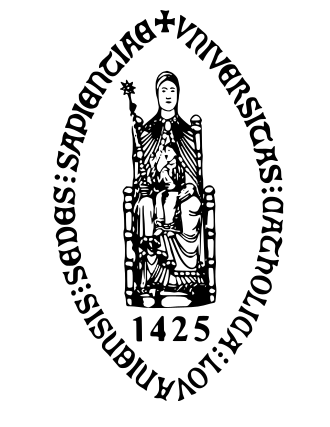
\includegraphics[height=3cm]{Images/logo_university.png}


\vspace{5cm}
\begin{center}
    \Huge{\rm{ \textbf{Encoding style: applying LoRA models in the context of Flemish architecture}}}\\
    \vspace{0.5cm}
    \Large
\end{center}
\begin{center}
    \Large{Academic year 2024-2025}
\end{center}
\vspace{0,5cm}



\vspace{7,5cm}
\begin{flushright}
    \large{Matijs Peeters r0854609}
    
\end{flushright}
\newpage
\thispagestyle{empty}
\vspace*{\fill}
\begin{center}
  \begin{minipage}{0.8\textwidth}
    \centering
    \justifying
    \noindent \copyright  2025 KU Leuven – Faculty of Engineering Science\\
    Published by Matijs Peeters, Faculty of Engineering Science,\\ Kasteelpark Arenberg 1 bus 2200, B-3001 Leuven\\
    All rights reserved. No part of the publication may be reproduced in any form by print, photoprint, microfilm, electronic or any other means without written permission from the publisher.\\
    This publication contains the study work of a student in the context of the academic training and assessment. After this assessment no correction of the study work took place.
  \end{minipage}
\end{center}
\vspace*{0pt}
\newpage

\tableofcontents

\addcontentsline{toc}{chapter}{Contents}
\chapter*{Abstract}
\addcontentsline{toc}{chapter}{Abstract}
Here comes the abstract
\newpage
\listoffigures
%\addcontentsline{toc}{section}{List of Figures}
\listoftables
%\addcontentsline{toc}{section}{List of Tables}
\newpage

\chapter{Introduction}
In de inleiding: alle termen en concepten kaderen + stukje literatuur tonen.

Algemene context: architectuurwereld in Vlaanderen.

Hier verwijzen naar een probleem. Kijk naar andere publicaties, en steel hun concept. Zet hier ook de REFERENTIE bij; je kan die later eventueel nog deleten.
Als die paper niet over het probleem gaat, en aantoont dat dat probleem er is, niet refereren.
over dat probleem mag ook al research gedaan zijn.

Suggereer een oplossing (die zich ergens anders evt al heeft voorgedaan) 
en evt een klein stuk van de oplossing voorstellen

bij mij: die LoRA modellen zijn nog niet op kleine schaal uitgetest.

Contributies (de wetenschappelijke bijdrage a/d wetenschap van wat ik doe)

Significantie \\
\\
Explain the broad context of the architectural world in Flanders
\\
\\
\section{The use of LoRA models in the world of architecture}
Although LoRA (\cite{hu_lora_2021}) emerged only in october 2021, several architects and architectural firms are already exploring its potential. Examples of these include Ismail Seleit (\cite{ismail_seleit_home_nodate}), who trains them on a variety of visual styles, and MVRDV (\cite{show_it_better_how_2024}), a global architectural office based in the Netherlands. \\
Several LoRA models have also been trained to replicate the style of large international offices of 'starchitects' such as Zaha Hadid \autocite{tangbohu_designed_2025}, Frank Gehry \autocite{laushine_frankgehryincuprum-lora_flux-architecture_2024}, and Rem Koolhaas (\cite{tangbohu_designed_2024}). LoRA can replicate the styles of these architects, however this is not the right way to use them, as Ismail Seleit explained in an episode of the podcast of Architech Network of 25 july 2024 \autocite{architech_network_ep_2024}. By attempting to replicate the existing style of an architectural office, it limits the potential of the generated images to inspire the architects of that same firm and provide them with new ideas.\\
\\
In the Flemish architectural landscape, there is a growing interest in using AI in the design process. This is illustrated by events like the New Year's reception of the 'Orde van Architecten' being centered around AI in architecture. On the smaller scale of Flemish architectural design firms, these models have not been tested yet. Flemish architects typically work very 'site-based', as opposed to imposing their own style on a new project every time they create a new one. This demands for a new approach, as it is hard for LoRA's to replicate this style.\\
\\
There are two considerations to make here:\\ 
1. Training a LoRA on an entire office does not yield interesting results;\\
2. Training a LoRA on a Flemish office in particular is a hard task, as there often are not many available images to train on.\\
\\
In an attempt to close both gaps and enable LoRA models to be applied in a useful way in the design processes of Flemish architects and architectural offices, this thesis defines a new type of concept to train a LoRA on: '\textbf{architectural design patterns}'. \\
%Philip Ball in his book 'The Self-Made Tapestry: Pattern Formation in Nature' defines these patterns in a simple and elegant way: ‘arrays of units that are similar but not necessarily identical, and which repeat but not necessarily regularly or with a well-defined symmetry’.\\
These patterns are visually distinctive patterns, materials or objects that Flemish architects might repeatedly use in their projects. LoRA models can easily understand these concepts, so that it is possible to train them with as little as 12-15 input images.\\
\\
A pattern has the following attributes: \\
- visually distinct\\
- rare but repeatable \\
- when trained in a LoRA and replicated in the generated images, it has a somewhat significant added contribution to the style of the architect.


\section{Research questions}\label{sec:research questions}

\textbf{1. What qualifies a mannerism that can be used to train a LoRA?\\~\\2. How does one train a LoRA to accurately reflect these mannerisms?\\~\\3. How might these LoRAs, trained on their own mannerisms, help Flemish architects in the architectural design process?}
%\chapter{Background}
\section{Diffusion models}
%There are several components that are used to create an image with AI. The most impactful one of these is the prompt: this is a piece of text that describes what the image should look like. Then there are other parameters added on top of that. The guidance scale (CFG) configures how strictly the model is pulled towards the prompt. \\
%For the scope of this thesis, only FLUX.1 [dev] will be used. This is a subjective choice, based on the quality on the model and how easy it is to train LoRA's for FLUX.1 [dev]. FLUX.1 [dev] is a guidance-distilled model, however FLUX.1 [schnell] is a timestep-distilled model, trained to generate good results in 1-4 interference steps.
\subsection{Definition}
Diffusion models are a type of generative artificial intelligence model which is as of 2024 most used for computer vision tasks, such as image generation, inpainting, image denoising and video generation. These models are trained on a large dataset of images and captions, learning to gradually denoise an image from pure noise to a high-resolution image.

\subsubsection{Training and inner workings of diffusion models}
The training and deploying of a diffusion model can be broken down into 3 stages: the forward diffusion process, the reverse diffusion process and finally image generation.\\ During the forward diffusion process, an image from the data set is transformed into pure noise. The most common method is by iteratively injecting Gaussian noise until the entire data distribution is gaussian \autocite{noauthor_what_2024}.\\ The reverse diffusion process is where the actual machine learning takes place: the model learns to perform the reverse of the noising steps of the forward process and thus learns to denoise pure gaussian noise into an image.
\begin{figure}[H]
    \centering
    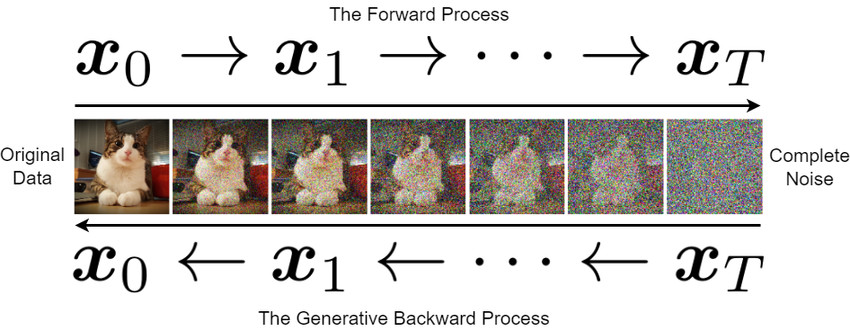
\includegraphics[width=0.8\linewidth]{Images/Background/The-forward-and-backward-processes-of-the-diffusion-model-The-credit-of-the-used-images.jpg}
    \caption{A visualisation of the forward and reverse diffusion process.}
    \label{fig:enter-label}
\end{figure}
Once the diffusion model has learned to estimate the amount of noise to be subtracted at each step, it can be used to generate new images. Inserting a slight element of randomness into this sampling process allows diffusion models to generate new images, that are not necessarily the same as the training images.
\subsubsection{Guided diffusion models}
A standard diffusion model can create high-quality variations of training images at random. Most practical uses of a diffusion model, however, require some control over the model's output. Guided diffusion models solve this problem by letting the user condition the generated images with a specific guidance.\\
The most common type of guided diffusion model is a text-to-image diffusion model, which lets users guide the generated images with a text prompt.\\
Methods for guided diffusion can be divided into two categories: Classifier-guided diffusion and classifier-free guidance. Classifier-free guidance has the benefit of enabling guidance for unseen image categories, whereas classifier-guided diffusion causes the diffusion model to only be able to condition outputs on the specific categories learned by the classifier.\\
Classifier-free guidance typically entails a two-stage model: in the first stage an embedding algorithm, like CLIP, creates an embedding for the prompt. In the second stage, a diffusion model uses this embedding to condition its output.
\subsubsection{Latent Diffusion models}
Conventional diffusion models are very good at generating images. However, they're slow and computationally expensive. These disadvantages were greatly reduced by latent diffusion models (\cite{rombach_high-resolution_2022}), starting with Stable Diffusion. \\
Rather than applying the diffusion process in pixel-space (i.e. directly to input images), these models first project the input to lower-dimensional latent space and apply the diffusion process there. The conversion of data from pixel space to latent space is done using a variational auto-encoder (VAE). The latent representation is then used as the input to the diffusion model. The output of the diffusion model, which is in the latent space, is finally upsampled to the desired image size using a decoder.
\subsection{Diffusion-based image generation models}
Over the last couple of years, Diffusion-based image generation models have become more and more popular, starting with the release of DALL-E by openAI in 2021. \\
\\
Generative image AI models come in two big categories: open-source and closed-source. Open-source models (e.g. stable diffusion and FLUX) can be downloaded through an online platform such as huggingface and used locally . Provided that one has access to a computer powerful enough to use these models, one can generate as many images as they like with these models. Closed-source models (e.g. Midjourney, Ideogram) ask a certain fee per month or per image generated, and can only be used through certain websites (e.g. fal.ai, replicate.com, midjourney.com, ideogram.ai).\\ 
\\

\subsubsection{Low-Rank Adaptation}
Low-rank adaptation, or LoRA in short, is a method to fine-tune models. Unlike full fine-tuning, this method uses less storage space; around a few hundred megabytes instead of many gigabytes. Training a LoRA takes on average only a few hours, depending on which hardware you use. These two properties make it an interesting tool to use for architects.

\subsubsection{ControlNet}
In the paper "Adding conditional control to text-to-image diffusion models", lvmin Zhang and coworkers from Stanford university introduced ControlNet, a 'neural network architecture to add spatial conditioning controls to large, pretrained text-to-image diffusion models' \cite{zhang_adding_2023}. ControlNet can be used to take the geometry from real images (such as sketches) and make the AI-generated images follow the same geometry. There are several 'preprocessors' which can freeze the geometry: in this paper, canny edge detection is used.
\subsection{Finetuning of diffusion models}
\subsection{Controlnet}
\chapter{Literature review}
This chapter reviews relevant literature in three key themes underpinning this research. First, it examines the role of images in architecture, not only as visual representations but as active agents in creative thinking and communication. Second, it examines Low-Rank Adaptation (LoRA) as an efficient method for fine-tuning text-to-image diffusion models, enabling targeted output images from small datasets, making the technique relevant for architectural applications. Finally, it situates the study within the context of Flemish architecture.

\section{The potential of AI-generated images in architecture}

% Papers die ik hier wil gebruiken:

% \cite{baudoux_benefits_2024}
% The technological partner (who is supplying images) is a relevant and potentially rich aid to ideation.

% Architects order images when the architect already has a premise of an idea, but it’s still vague, and he/she’s looking for inspiration to find out exactly what form this idea will take.

% The proposal was to avoid prompts (andere bron hiervoor?), but they found that there is a real need to be able to order specific images, as the designers made a real usage of this provided function. "The advantage of our system over text-to-image AI generators is that the “prompt” can simply be composed of three or four keywords, while the technological partner knows the project being designed and the creative direction in which the architect is heading. So there’s no need to specify all the details in a complex prompt."

% "... a need previously unknown or underestimated in the literature: the need to evaluate sketched ideas by means of images simulating their real-life rendering, as well as the need for inspiration to materialize the premises of ideas that are still vague."

% \cite{paananen_using_2024}
% "Through standardized questionnaires on creativity support tools and group interviews, we learned that image generation could be a meaningful part of the design process when design constraints and imaginative ideation are carefully considered. Generative tools support the serendipitous discovery of ideas and an imaginative mindset, which can enrich the design process."

% "In a 2013 lecture, the renowned contemporary architect Bernard Tschumi explained the role of visual media in architecture as “It is not about the images, it is what the images do.” [31]. As architecture can be seen as a field that communicates through images, it is the effect of the images that matter and what political and social impact they have. Therefore, image generation could be understood as a part of a more context-aware creative practice."

% \cite{castro_pena_artificial_2021}
% "There is a remarkable increase in the number of publications on the topic over time from 2015 onwards, with 85\% growth in the last 5 years compared with previous years"

% \cite{duran_review_2025}
% "Advances in open text-to-image and image-to-image diffusion models can democratize the design process by reducing the need for powerful hardware for realistic renderings or 3D modeling, enabling co-creation with AI in the design of new facades."

% \cite{rombach_high-resolution_2022}
% I want to cite this paper because it handles (latent) diffusion models, the kind of models I use in my thesis.

% In the world of AI-assisted design (AIAD), ...

% In the paper 'The benefits and challenges of AI image generators for architectural ideation: Study of an alternative human-machine co-creation exchange based on sketch recognition' \cite{baudoux_benefits_nodate}, the wizard of Oz-technique was used to emulate a design situation where the 'wizard' is regularly showing images to the architects. This paper shows that this kind of stimulation can help architects design. In this thesis, a similar approach is used to design together with architects. However, the technique is already developed. The researcher only serves as a middle person, communicating between the AI-model interface and the architect.
\subsection{The increasing influence of images}
Throughout its history, architectural practice has been underpinned by the use of visual representations - such as sketches, photographs, and images - to communicate ideas across all stages of the architectural process, from initial concept development to construction. In recent years, the role of images has considerably increased, especially within the architectural design phase, where they do not only function as illustrations, but can take an active role, providing architects with relevant references and stimulating novel ideas (\cite{bergera_architecture_2022}; \cite{halin_three_2003}).

\subsection{AI image generation}
Following the strong increase of research and development regarding artificial intelligence (AI), architects and researchers alike have showed interest in architectural AI applications, initially mainly focusing on attempting to converge on a single optimized outcome. However, since 2015, the overall emphasis of research lies more and more on interactive, generative approaches, that expand the designers solution space (\cite{castro_pena_artificial_2021}).\\
%Highlighting that architects are willing to embrace this new technology.
\subsection{Diffusion models}
Several approaches exist for generating images using artificial intelligence. However, probabilistic diffusion models (DDPMs)(\cite{ho_denoising_2020}) outperform other generative AI technologies such as generative adversarial networks (GANs),  and Variational Auto-Encoders (VAEs). Especially latent diffusion models (\cite{rombach_high-resolution_2022}) have greatly enhanced the quality and efficiency of image generation, by reducing the dimensionality of the image data from pixel space to latent space, requiring less memory to create high-quality outputs (\cite{li_generative_2025}). There have especially been a lot of developments in text-to-image generation models (\cite{zhang_text--image_2023}), which use text as input and generate images as outputs. Examples include MidJourney (\cite{noauthor_midjourney_nodate}), FLUX (\cite{noauthor_black-forest-labsflux1-dev_2025}), Stable Diffusion (\cite{rombach_high-resolution_2022}), and Imagen (\cite{noauthor_imagen_nodate}), among others. These models facilitate generating images from text prompts in seconds, giving rise to a lot of potential use cases in the architecture industry.
\subsection{The effect of text-to-image models on the architectural design process}
Text-to-image models have been found to support the serendipitous discovery of novel ideas and an imaginative mindset, both of which can significantly enrich the design process (\cite{paananen_using_2024}). The images themselves do not necessarily serve as purely representational tools, but can provide a lot of creativity, especially in the early, conceptual stages of design.\\
\\
An important limitation of these tools, however, is that they can't conform very well to specific building regulations. This further strengthens the notion that these models work best in the early stages of design. Architects actually use it in this way: when they can order images, they do it when they already "have a premise of an idea, but it’s still vague, and he/she’s looking for inspiration to find out exactly what form this idea will take" (\cite{baudoux_benefits_2024}).\\
\\
AI text-to-image models relying heavily on text prompts (\cite{tan_using_2024}), another significant challenge is the skill treshold associated with effective prompt engineering (\cite{paananen_using_2024}). However, prompts are still needed to some extent; architects who are using AI-generating tools in their design process frequently express the need to order specific images, where a simple prompt is still needed (\cite{baudoux_benefits_2024}). This highlights the need to be able to control the generated images to some extent.

Apart from generating new ideas, there is also a need to validate sketched concepts by realistic imagery based on architects' sketches, enabling validation of early ideas and proposals. Thus, text-to-image and image-to-image generation tools can not only function as a source of inspiration, but also as a tool for testing design decisions (\cite{baudoux_benefits_2024}).

\section{Low-Rank Adaptation of diffusion models}

\subsection{Fine-tuning of diffusion models}
Most widely-spread diffusion models are examples of 'foundation models': they are trained on huge datasets and can handle a wide variety of image generation requests. However, for very specific queries that are not present in the general dataset, these models don't perform very well. An example is the replication of a certain architectural style, which, if possible, would make these tools more interesting for architects, as they could tailor them more to their needs. One possible solution would be to retrain the entire model; however, this would bring a high cost and require a lot of effort. 'Fine-tuning' of diffusion models can offer a more feasible solution, by adapting a pre-trained diffusion model to a specific task. 
\subsection{Low-Rank Adaptation}
Several fine-tuning techniques have already been developed, such as full finetuning, textual inversion (\cite{gal_image_2022}), LoRA (\cite{hu_lora_2021}), hypernetworks (\cite{huang_continual_2021}) and DreamBooth (\cite{ruiz_dreambooth_2022}). Dreambooth usually performs best among these methods, because it fine-tunes the entire model (\cite{chen_generating_2023}). For recent diffusion models, though, this would require a lot of storage space: as an example, the file size of FLUX.1 [dev] is 23.8 gigabytes (GB) (\cite{noauthor_black-forest-labsflux1-dev_2025}), meaning the finetuned DreamBooth-model could easily exceed 25 GB. \\
Although not the very best method, LoRA could be a promising fine-tuning technique for architects because of its parameter efficiency (\cite{yang_low-rank_2024}). The finetuning process for LoRA models (or LoRAs, in short) is relatively fast and the LoRA model is not too large.

\subsection{The use of LoRAs in architecture design}
Indeed, there are various architects and firms who are already actively researching the possibility of  implementing LoRAs in their design process. Examples of these include Ismail Seleit (\cite{architech_network_ep_2024}), who is an associate architect at Foster + Partners and trains LoRAs on a variety of visual styles and concepts. The Dutch office MVRDV, a globalized architectural office based in the Netherlands, is also experimenting with this technology (\cite{show_it_better_how_2024}). \\
Several LoRA models have also been trained by online users, to replicate the style of large international offices of 'starchitects' such as Zaha Hadid \autocite{tangbohu_designed_2025}, Frank Gehry \autocite{laushine_frankgehryincuprum-lora_flux-architecture_2024}, and Rem Koolhaas (\cite{tangbohu_designed_2024}). 

%LoRA can replicate the styles of these architects, however this is not a very useful way to harness them. By attempting to replicate the existing style of an architectural office, it limits the potential of the generated images to inspire the architects of that same firm and provide them with new ideas. A more interesting approach would be to train project-specific LoRAs (\autocite{architech_network_ep_2024}).\\

\section{The Belgian architectural landscape}

\subsection{Historical context}
In the mid-20th century, Belgium's modern architectural identity was often described in unflattering terms: architect Renaat Braem famously described his home country as the 'ugliest country in the world' (\cite{braem_het_1968}).\\
Since then, the architectural landscape of Belgium has undergone significant transformation: particularly over the last two decades, key institutions such as Team Flemish Government Architect (\url{https://www.vlaamsbouwmeester.be/nl}) and the Flemish Architecture Institute (VAi) (\url{https://www.vai.be/en}) have had a substantial influence on Belgian architectural practice, which has its effect: Belgian architecture has gained international recognition for its context-specific approach (\cite{wainwright_flanders_2022};\cite{antonissen_continuity_2022}).

\subsection{Current situation}
Today, many Belgian, and especially Flemish, architects deliberately avoid maintaining a fixed 'personal' style in their architectural designs. Instead, they allow the architectural expression of each new project to be inspired by the site, the program and the social context (\cite{de_caigny_flanders_2024}). The aim of architecture is not to create a uniform portfolio, but rather to achieve a 'local identity' for each project. "In this way, Flemish building culture illustrates an understanding of architecture as a contribution to the generic architectural or urban tissue, not as an artefact or monument in itself." (\cite{antonissen_continuity_2022}, as cited from  \cite{avermaete_rereading_2016}).

\chapter{Development process}
\todo{intro schrijven}

\section{Diffusion model used: FLUX.1 [dev]} \label{sec:Models used}
The diffusion model used in this thesis is called FLUX.1 (\cite{black_forest_labs_announcing_2024}), a text-to-image diffusion model released on August 1, 2024, in three variants: FLUX.1 [pro], [dev], and [schnell]. Of these three variants, only [dev] and [schnell] have open-source weights and thus support local use and fine-tuning via low-rank adaptation (LoRA).\\
Following preliminary experimentation, only FLUX.1 [dev] is used in this thesis, because of its superior integration with Ostris' FLUX.1 [dev] LoRA trainer. LoRAs trained with the [dev] trainer also function with FLUX.1 [schnell], but yield lower-quality output images. Training LoRAs specifically for FLUX.1 [schnell] is also possible, although one would need to use an adapter for that (the adapter can be found on \url{https://huggingface.co/ostris/FLUX.1-schnell-training-adapter}{https://huggingface.co/ostris/FLUX.1-schnell-training-adapter}). This option was not tested.
\section{Image generation techniques}
\subsection{Text-to-Image}
\todo{kleine intro bij schrijven}
\subsubsection{ChatGPT} \label{sec:ChatGPT}
To streamline the prompt engineering process, the researcher trained a custom GPT named 'LoRA prompt generator' (\href{https://chatgpt.com/g/g-68279d68896c81918191491b79281abe-lora-prompt-generator}{link}) to output high-quality prompts consisting of a six-part structure. A GPT is a custom version of ChatGPT that can follow specific instructions (\cite{openai_introducing_2023}). This option was chosen because of the combination of accessibility (since GPTs are easy to configure without knowing a lot about large language models) and effectivity.\\
The recommended models to use for this GPT are GPT-o3 and GPT-o4-mini \footnote{Since the release of GPT-5 on august 7, 2025, these models are not directly accessible anymore. It is therefore recommended to use GPT-5 Thinking.}, because they are able to directly integrate images into their chain of thought (\cite{openai_introducing_2025}, section 'Thinking with images').\\
The researcher can write a prompt in natural language, and the GPT reformulates it into a six-part prompt following a fixed structure. This structure facilitates easier analysis of the prompts. Table \ref{tab:gptprompt} dissects a representative output generated by the GPT to illustrate the structure. \\

\begin{table}[H]
  \centering
  \begin{tabular}{l p{0.6\textwidth}}
    \toprule
    Structure & Prompt segment \\
    \midrule
    1. Trigger word 
    & Stampbeton \\
    2. Subject
    & shapes the rugged elegance of a countryside farmhouse, where the front facade stands defined by sturdy stamped concrete walls that echo the texture of hand-laid stone. \\
    3. Attributes on the subject
    & A gently slanted roof clad in red shingles crowns the structure, lending a traditional warmth that contrasts the cool, tactile mass of the concrete below. On the front elevation, a single wooden door punctuates the left side, its weathered grain harmonizing with the rustic palette, while a solitary window on the right offers a glimpse into the home’s quiet interior, framed by thick concrete reveals. \\
    4. Surroundings
    & The house is nestled into a soft rural clearing, flanked by wild grasses and a gravel path that leads up to the entrance, with distant hedgerows and fencing marking the rhythm of nearby fields. \\
    5. Atmosphere 
    & Overhead, a wide expanse of blue sky peeks through the rolling coverage of dense, moody clouds, diffusing the daylight into a serene, shadowless glow. \\
    6. Style 
    & Rendered in photorealistic style, the scene captures the raw materiality and quiet strength of this rural retreat, balanced by a subtle, cinematic atmosphere. \\
    \bottomrule
  \end{tabular}
  \caption{The six-part structure used to generate every prompt in this thesis.\\}
  \label{tab:gptprompt}
\end{table}
Users can edit the output prompt to their preference, reducing the workload compared to writing a high-quality prompt from scratch. \\
Because every image generated in this thesis is a pair (with and without LoRA; see section \ref{sec:Workflow used to generate images}), the GPT was designed to output two prompts: one with the trigger words and one with their English equivalents that the base model FLUX.1 [dev] can interpret. This ensures the comparison is as fair as possible.

\begin{table}[H]
    \centering
    \begin{tabular}{ll}
        \toprule
         Stampbeton & Stamped concrete\\
         3Deffect & 3D effect\\
         Geleding & Division \\
         Modulariteit & Modularity\\
         Ghoek & Curvature\\
         Plintwerking & Plinth effect\\
         \bottomrule
    \end{tabular}
    \caption{All of the trigger words and their English counterpart.}
    \label{tab:triggerwords}
\end{table}

\subsection{Image-to-Image}
\subsubsection{ControlNet}
To generate images based on sketches or images of the architects, ControlNet (\cite{zhang_adding_2023}) was used, a technique to add compositional control to large diffusion models such as FLUX. The ControlNet model used in this thesis is the 'union pro' model by Shakker Labs (\url{https://huggingface.co/Shakker-Labs/FLUX.1-dev-ControlNet-Union-Pro/tree/main}), which includes several preprocessors.
\section{Interface used to generate images} \label{sec:Workflow used to generate images}
\subsection{ComfyUI}
\sloppy
The interface used to generate images in this thesis is called ComfyUI (\href{https://www.comfy.org/}{comfy.org}), an open source node-based user interface. Alternatives such as Automatic1111, Fooocus and InvokeAI were considered; however, ComfyUI was selected due to two primary advantages. 
\begin{enumerate}
    \item Reproducability: generated images embed the complete 'workflow' used to create it (see \href{https://docs.comfy.org/development/core-concepts/workflow}{docs.comfy.org} for further explanations). Since reproducability is an important aspect of research, this is a very attractive feature, as it allows researchers to retrace how every AI-generated image in this thesis was created.
    \item Customizability: by using fundamental building blocks ('nodes', see \href{https://docs.comfy.org/development/core-concepts/nodes}{docs.comfy.org}), ComfyUI users can create their own workflows to meet various needs, and can also write and implement custom nodes to further customize workflows.
\end{enumerate}
Figure \ref{fig:comfy interface} illustrates the default ComfyUI workflow, which can generate one image from a positive and a negative prompt.
\begin{figure}[H]
    \centering
    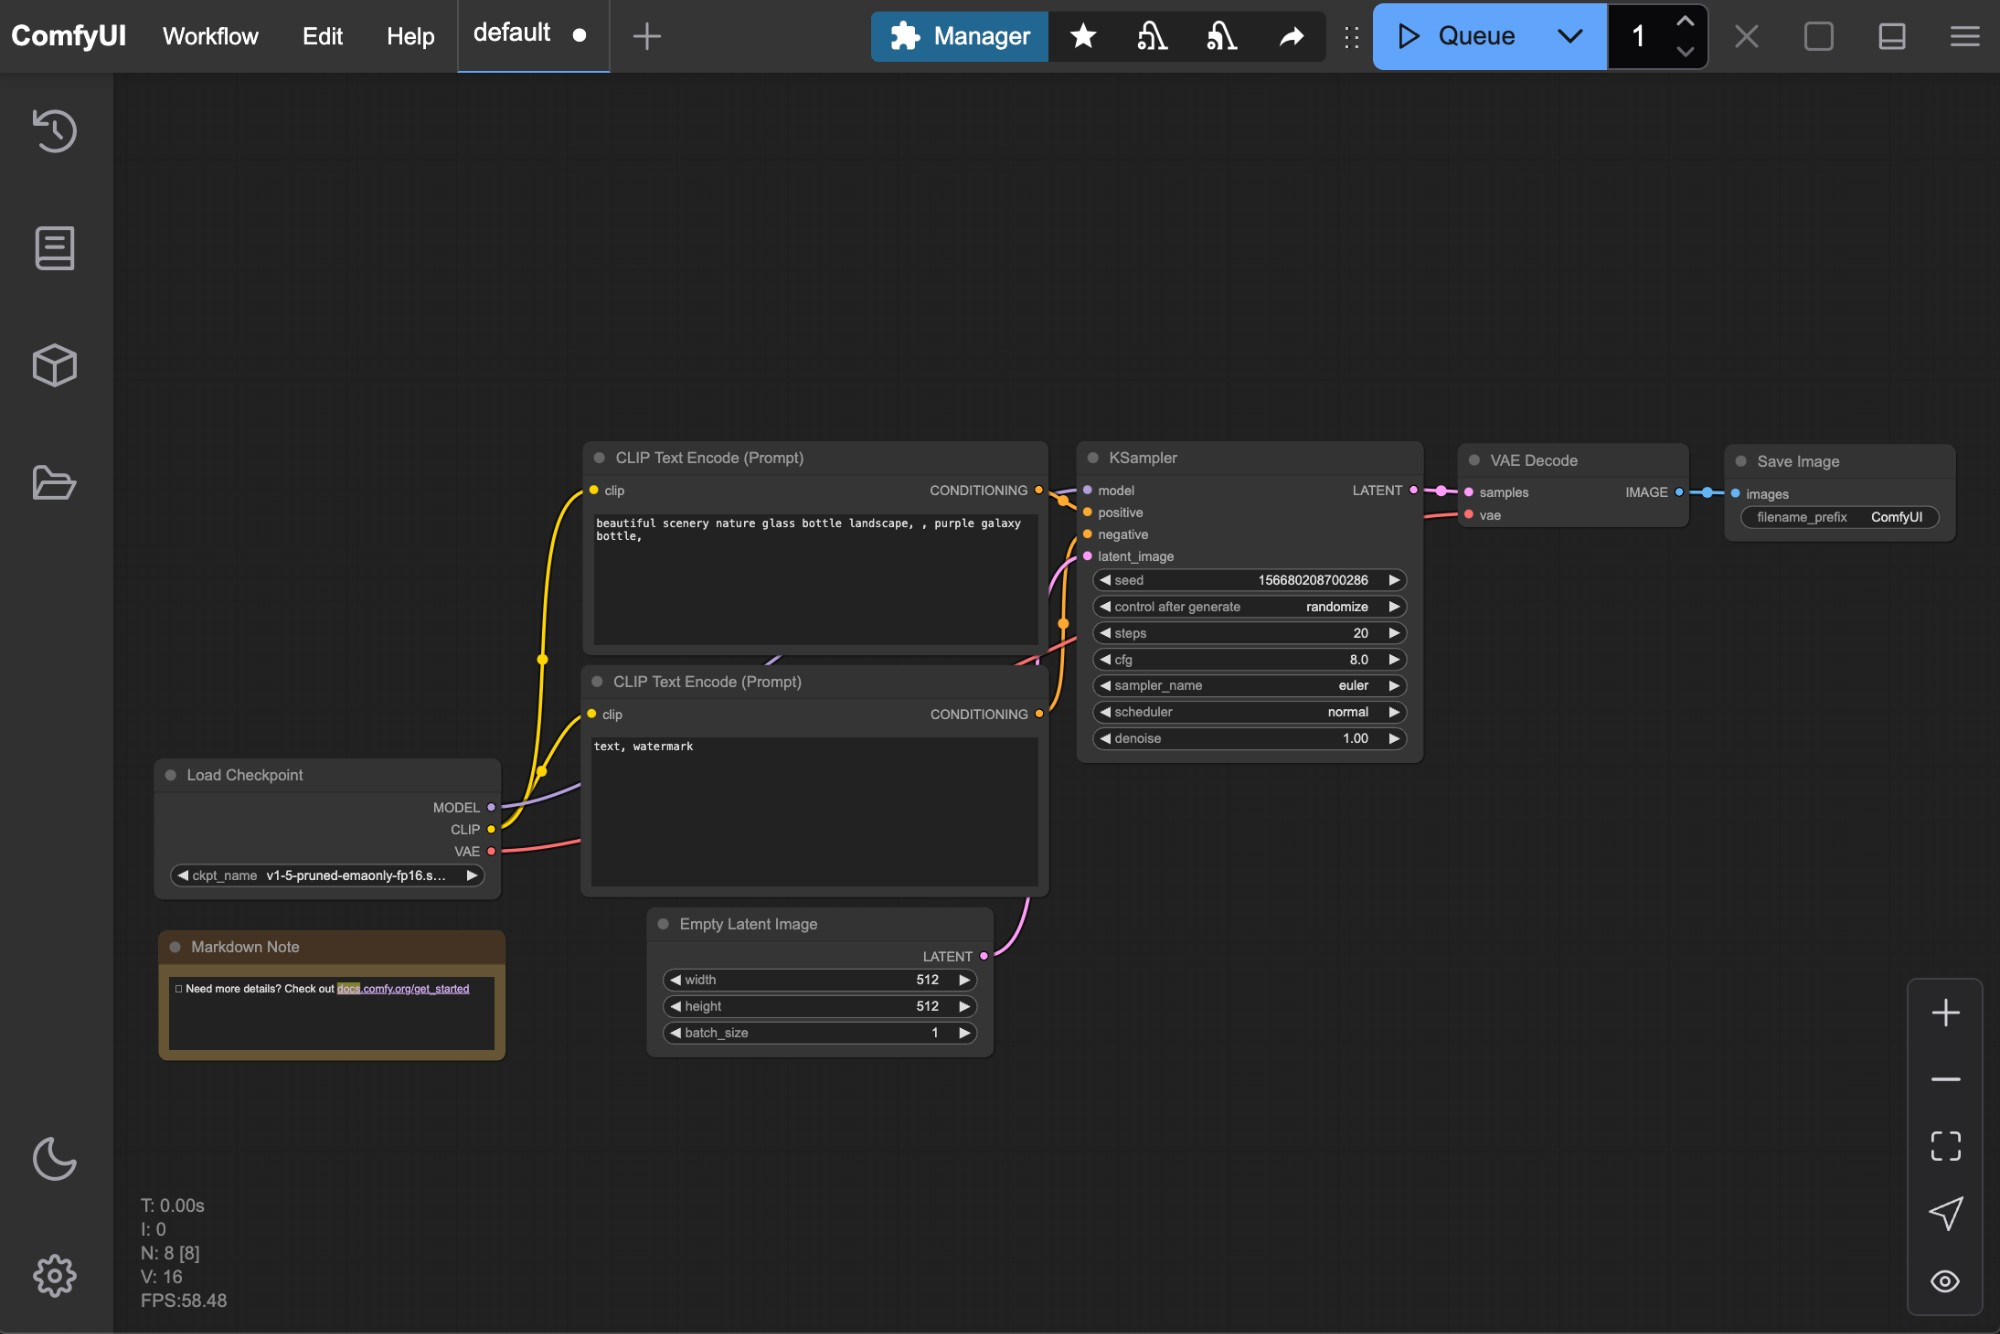
\includegraphics[width=0.8\linewidth]{Images//Methodology/comfyui_new_interface.jpg}
    \caption{The default workflow when starting ComfyUI.}
    \label{fig:comfy interface}
\end{figure}

To generate images, the researcher employed an online service called \textbf{ThinkDiffusion} (\href{https://www.thinkdiffusion.com/}{thinkdiffusion.com}) and rented a server with 48 gigabytes of video random-access memory (VRAM), which is capable of generating one image in about 30 seconds when using FLUX.1 [dev]. The version of ComfyUI used is ComfyUI v0.3.44, the latest available in July 2025.
\subsection{Workflow used in this thesis}
To generate all of the images in this thesis, the researcher employed a custom workflow developed by Swedish art director and youtuber Sebastian Kamph(\cite{sebastian_kamph_flux_2024}), which enables the use of ControlNets in combination with FLUX. To isolate and highlight the effect of LoRA on the generated output images, the workflow was modified into a new version (figure \ref{fig:own comfy workflow}) that generates two images per execution: one with LoRA enabled and one without. All other parameters, such as prompts and seed values, are held constant. Each time the workflow is executed, two images are simultaneously generated and displayed in the nodes on the bottom right of the workflow.\\ 
\begin{figure}[H]
    \centering
    \href{https://github.com/matijspeeters/Thesis/blob/main/Images/Methodology/workflow%20(5).png}{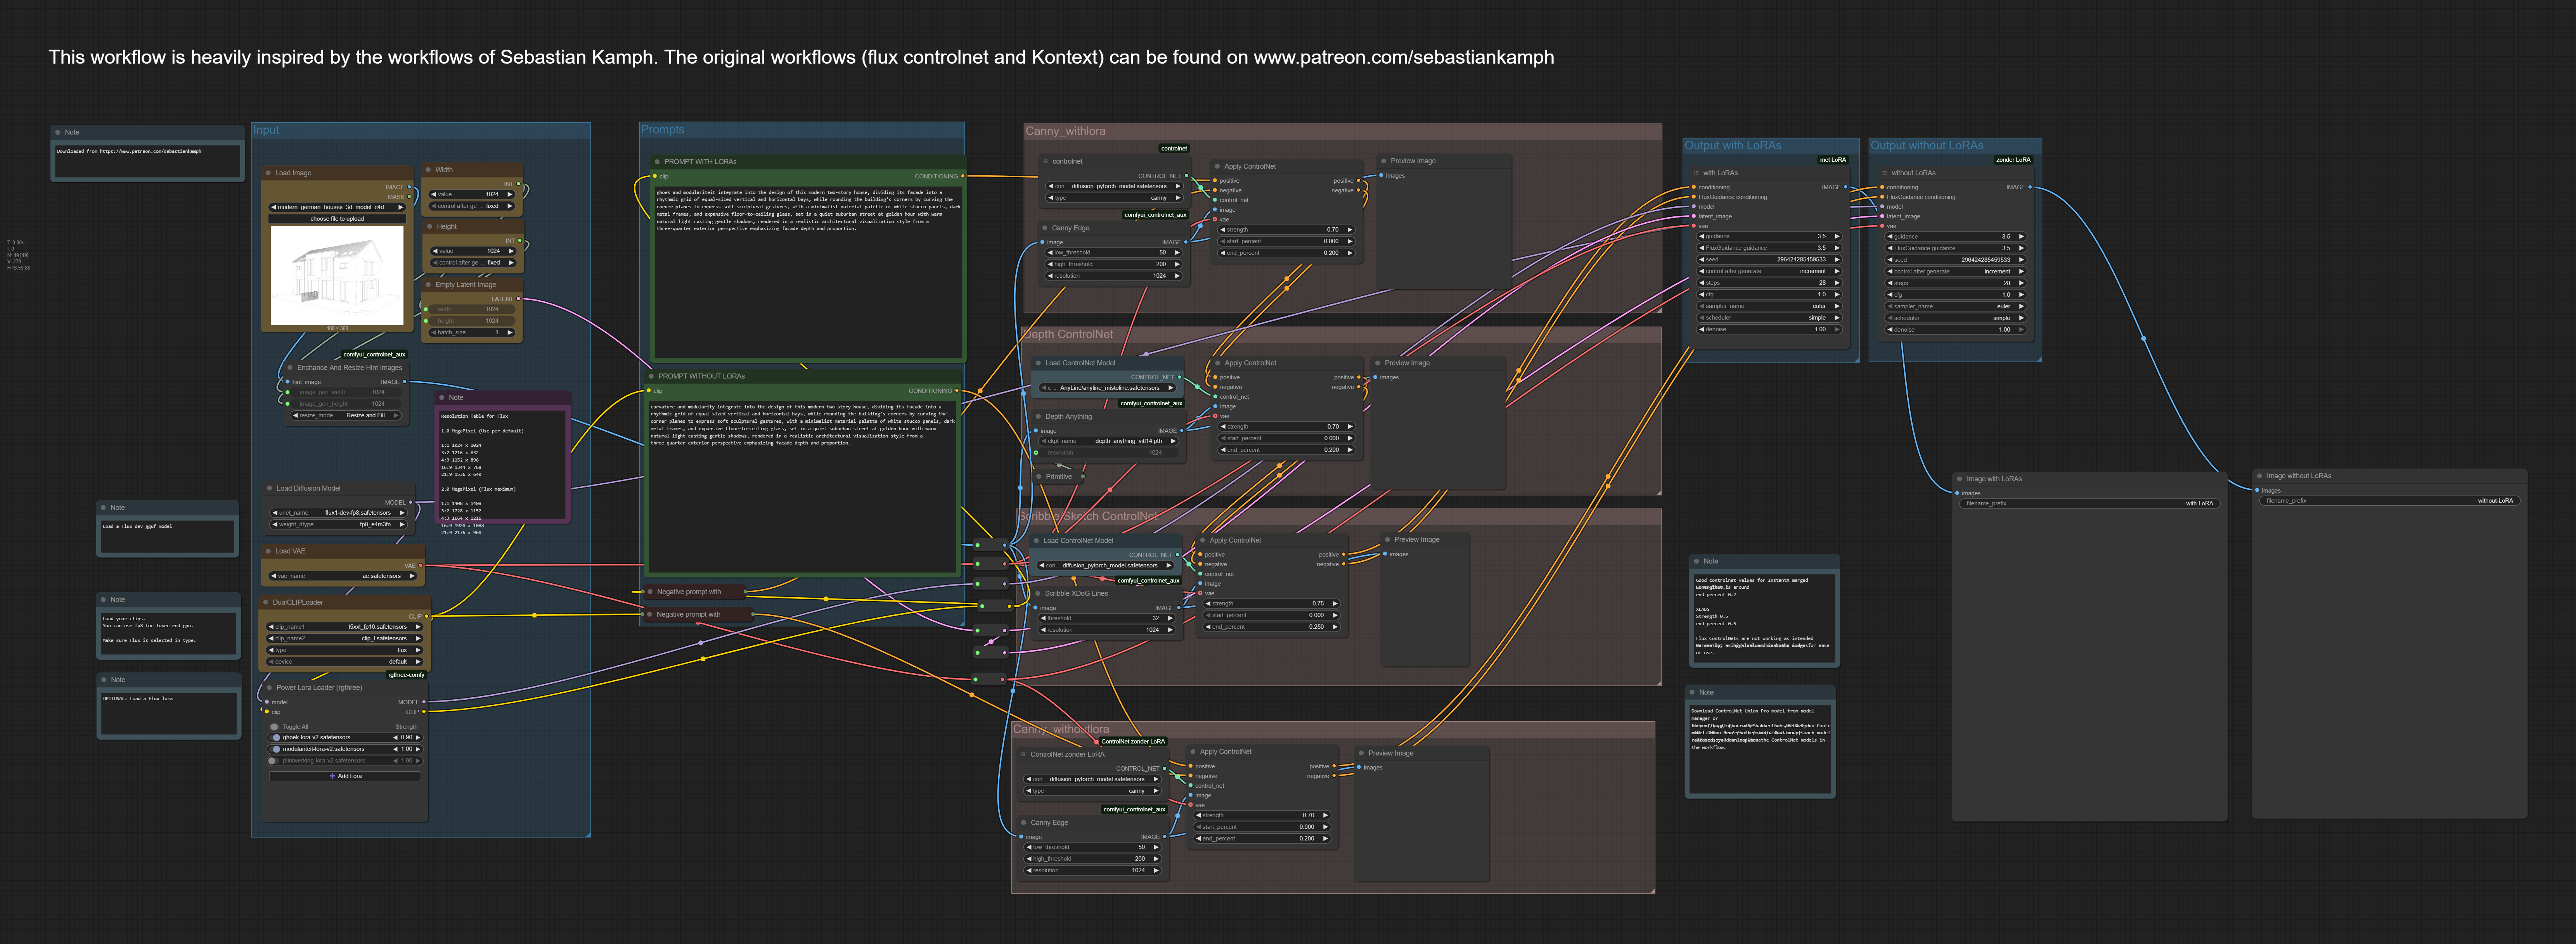
\includegraphics[width=\linewidth]{Images/Methodology/workflow (5).png}}
    \caption{The modified ComfyUI workflow, used to generate every image in this thesis.}
    \label{fig:own comfy workflow}
\end{figure}
\chapter{Methodology}

The research questions are addressed via an exploratory study involving Flemish architecture offices. The methodology is outlined in five sequential stages (figure \ref{fig:methodologycasestudy}):

% DMOA (\href{https://www.dmoa.be/}{dmoa.be}) and LAVA (\href{https://lava-architecten.be/}{lava-architecten.be}). \\

\begin{itemize}
    \item Semi-structured \textbf{interviews} with one partner from each office, to identify and agree upon the specific mannerisms to be trained on (section \ref{sec:Interviews});
    \item \textbf{Collecting} datasets of images to train the LoRAs (section \ref{sec:Finalized training datasets});
    \item \textbf{verifying} those images with the architects (section \ref{sec:Finalized training datasets});
    \item \textbf{Training} LoRAs on these datasets (the methodology for training the LoRAs is explained in section \ref{sec:LoRA training methodology});
    \item \textbf{Evaluating} the resulting LoRAs in two settings: a structured design process and an unstructured process. (section \ref{sec:Evaluation sessions})
\end{itemize}
\begin{figure}[H]
    \centering
    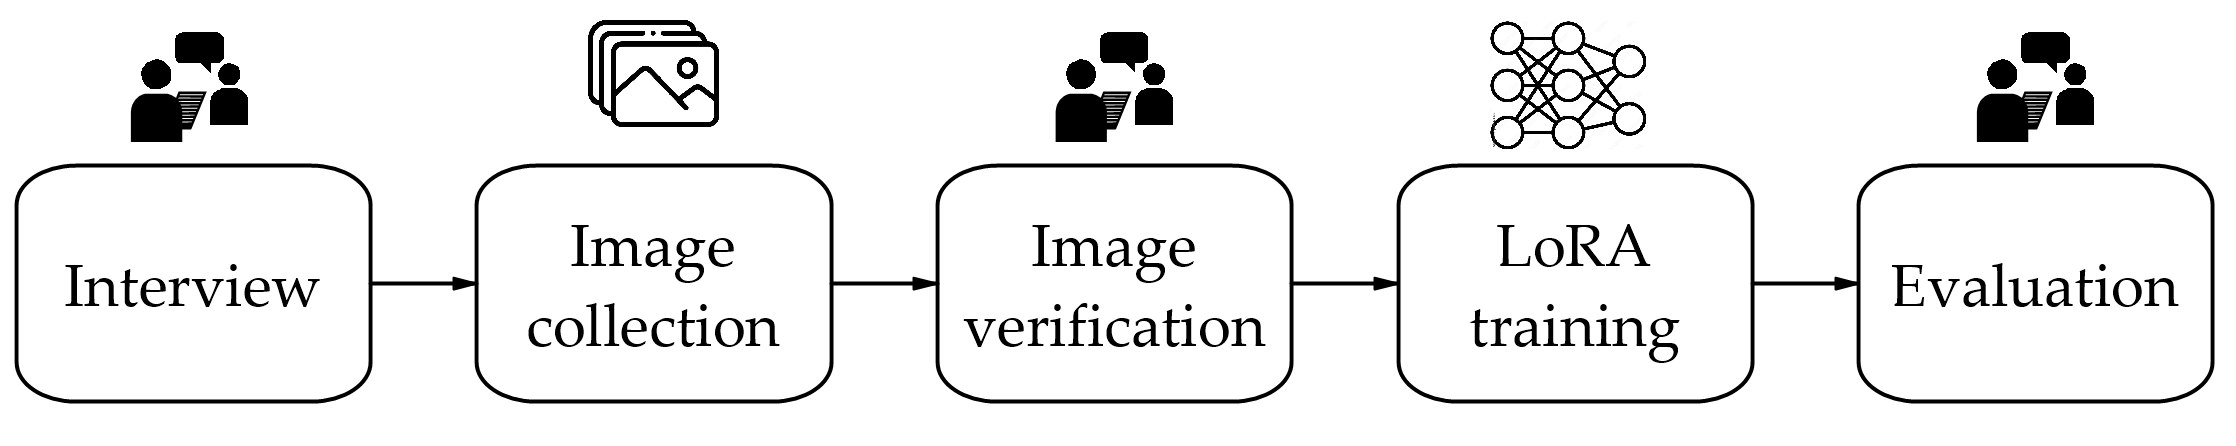
\includegraphics[width=\linewidth]{Images/Methodology/Methodology.jpg}
    \caption{The methodology of the case study.}
    \label{fig:methodologycasestudy}
\end{figure}

\section{Interviews} \label{sec:Interviews}

The selection of the mannerisms was based on semi-structured interviews with the architects (one partner from DMOA and one partner from LAVA). Based on these interviews, six mannerisms (3 per architect) were selected to align with the architects' preferences and expectations.\\ The interviews covered personal style, the role of mannerisms in their design, and prospective uses of LoRA in their design process, after which candidate mannerisms were proposed, based on review of the architects' projects and own expertise on training LoRAs. The architects then selected the 3 mannerisms they thought most useful.

\section{Image selection and verification} \label{sec:Finalized training datasets}
LoRA training requires a diverse collection of high-quality images that capture the concept in diverse environments, lightings and camera angles (\cite{deepfates_fine-tune_2024}).\\
To ensure equal influence on the model, all images were resized to 1024 x 1024 px using the online image resizer BIRME (https://www.birme.net/), matching the default output format for FLUX.1. The end result of the collection phase was a selection of 15-19 images for each LoRA.\\~\\
Prior to LoRA training, both architects reviewed the selected images through a google form, rating each image from 1 (poor representation of the concept) to 3 (clear representation). After a brief online call where the architects clarified their intentions, the image set was revised: certain images were removed and new ones added to better reflect the concept. The newly added images were not reviewed by the architects: it was assumed that the discussion had provided sufficient understanding of the architects' vision to select appropriate images.\\

\subsection{Finalized datasets for DMOA}
\subsubsection{Stampbeton}
The first LoRA trained for the office of DMOA is meant to replicate the material stamped concrete ('stampbeton' in Dutch). The architects have developed and patented a specific mixture of materials to create their version of the material.\\
% To train this LoRA, several images were used of two projects by DMOA: Farmer's House and KRUUL. Next to that, images of Peter Zumthor's Bruder Klaus Field Chapel in Mechernich, Germany, as well as an interior application of the material were used.\\
After validation, one image (figure \ref{fig:stampbetonomittedimage}) was left out of the original dataset: the dirty spots on the concrete in the image were too prominent, and the concrete did not sufficiently represent the typical horizontal layering of stamped concrete.
\begin{figure}[H]
    \centering
    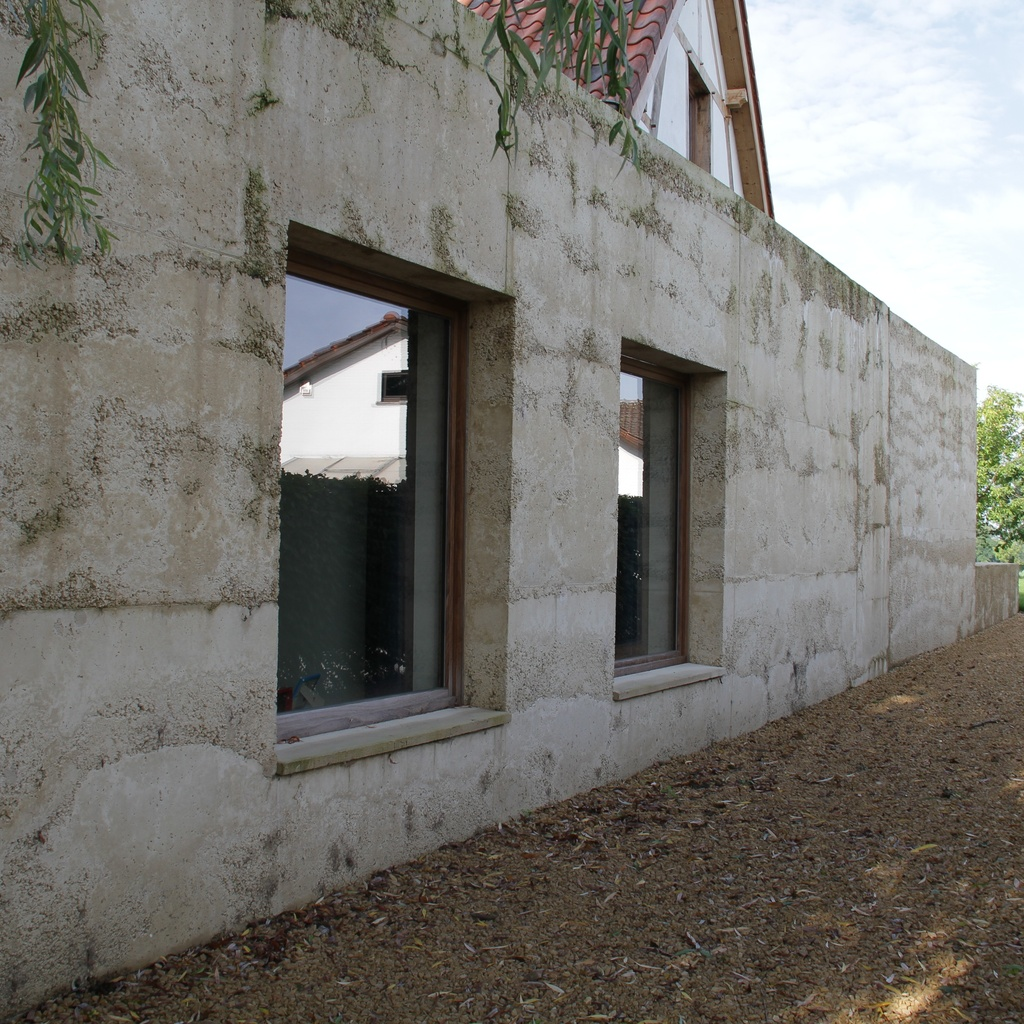
\includegraphics[width=0.24\linewidth]{Images//LoRAs//STAMPBETON/12.jpg}
    \caption{The image removed from the original dataset.}
    \label{fig:stampbetonomittedimage}
\end{figure}
Figure \ref{fig:gridstampbeton} portrays the training images for this LoRA.
\newcommand{\cellwidth}{0.24\textwidth}
\begin{figure}[H]
  \centering
  \resizebox{\textwidth}{!}{%
    \begin{tabular}{@{}ccccc@{}}
      % Row 1: images 1–5
      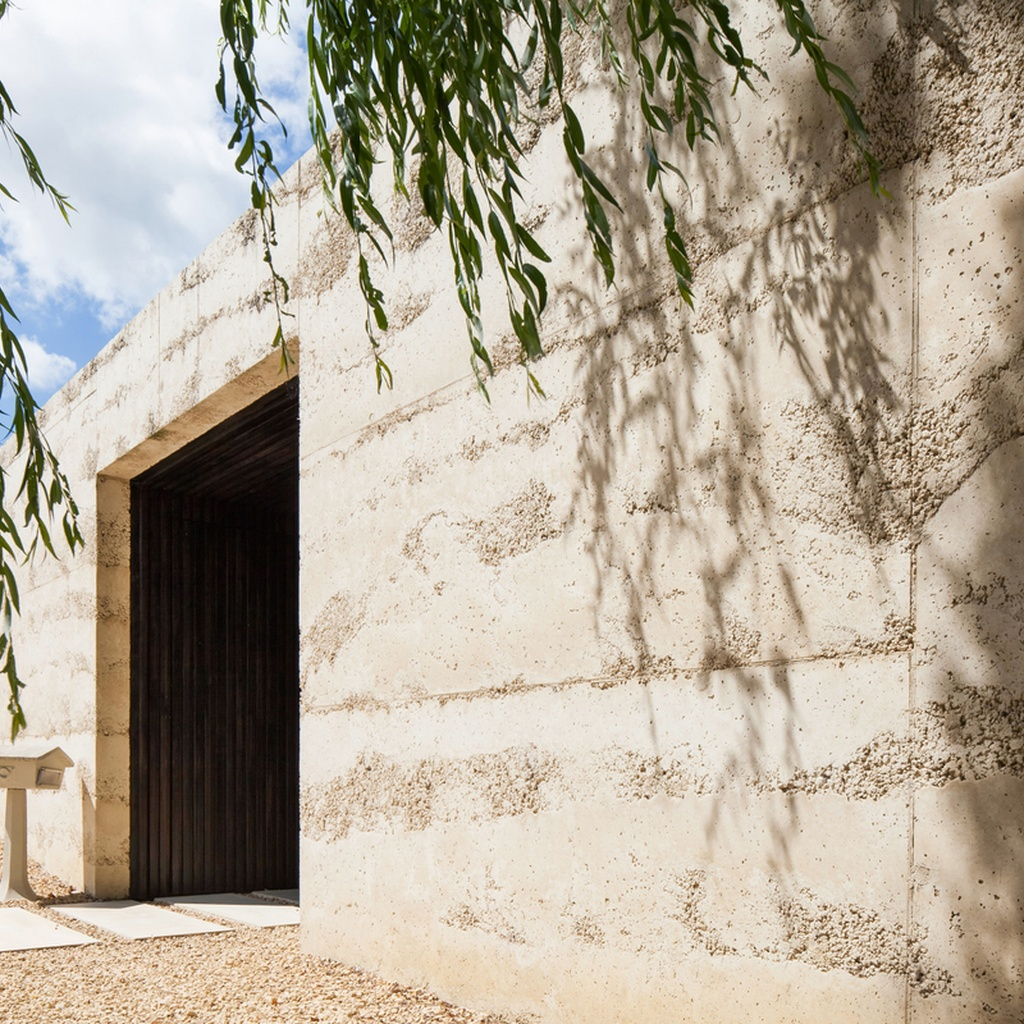
\includegraphics[width=\linewidth]{Images/LoRAs/STAMPBETON/Training_images/1.jpg} &
      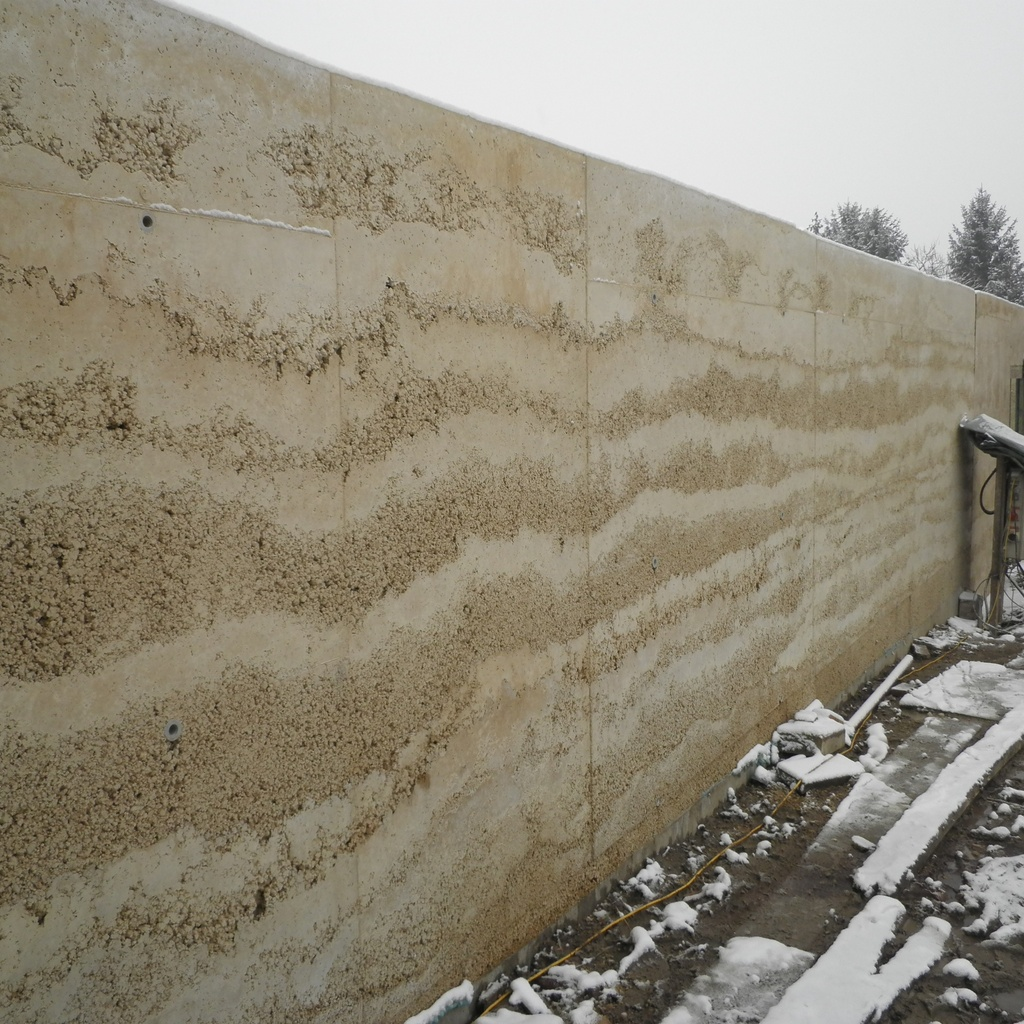
\includegraphics[width=\linewidth]{Images/LoRAs/STAMPBETON/Training_images/2.jpg} &
      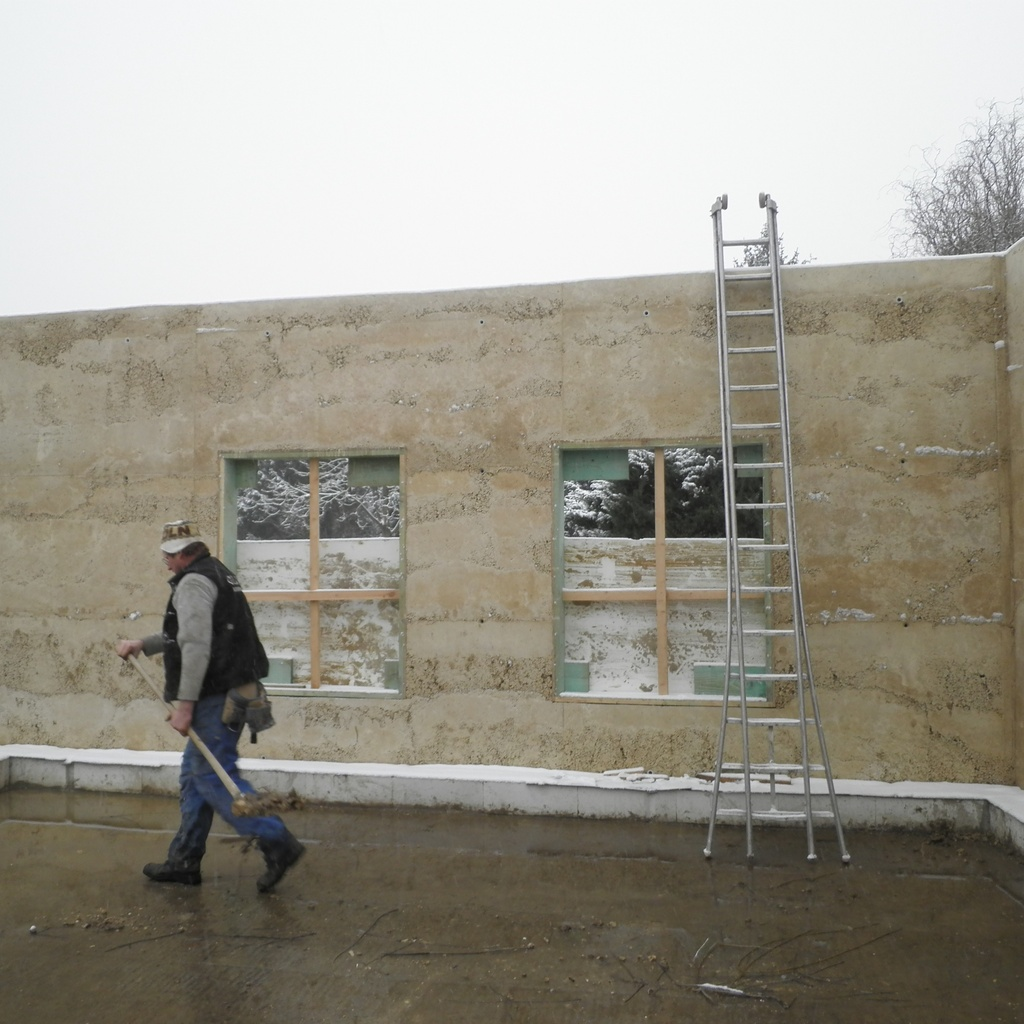
\includegraphics[width=\linewidth]{Images/LoRAs/STAMPBETON/Training_images/3.jpg} &
      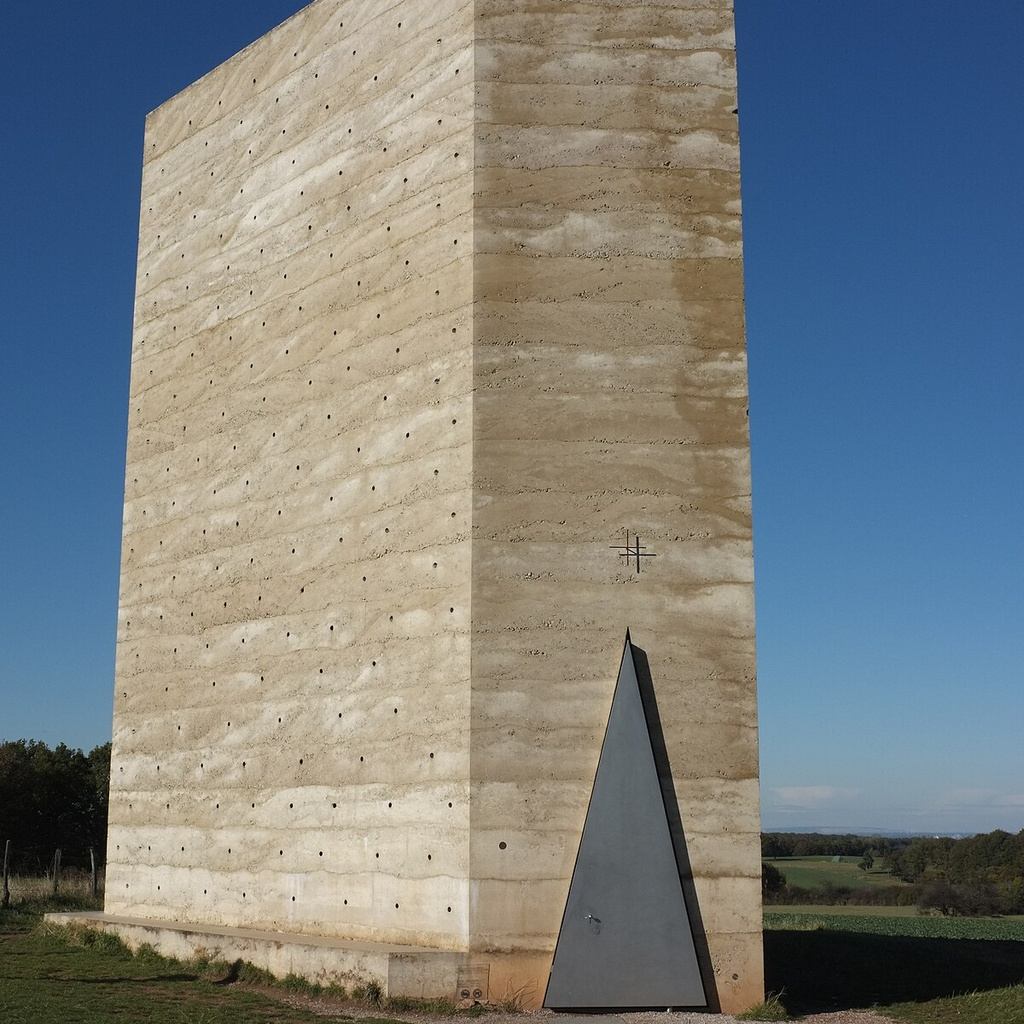
\includegraphics[width=\linewidth]{Images/LoRAs/STAMPBETON/Training_images/4.jpg} &
      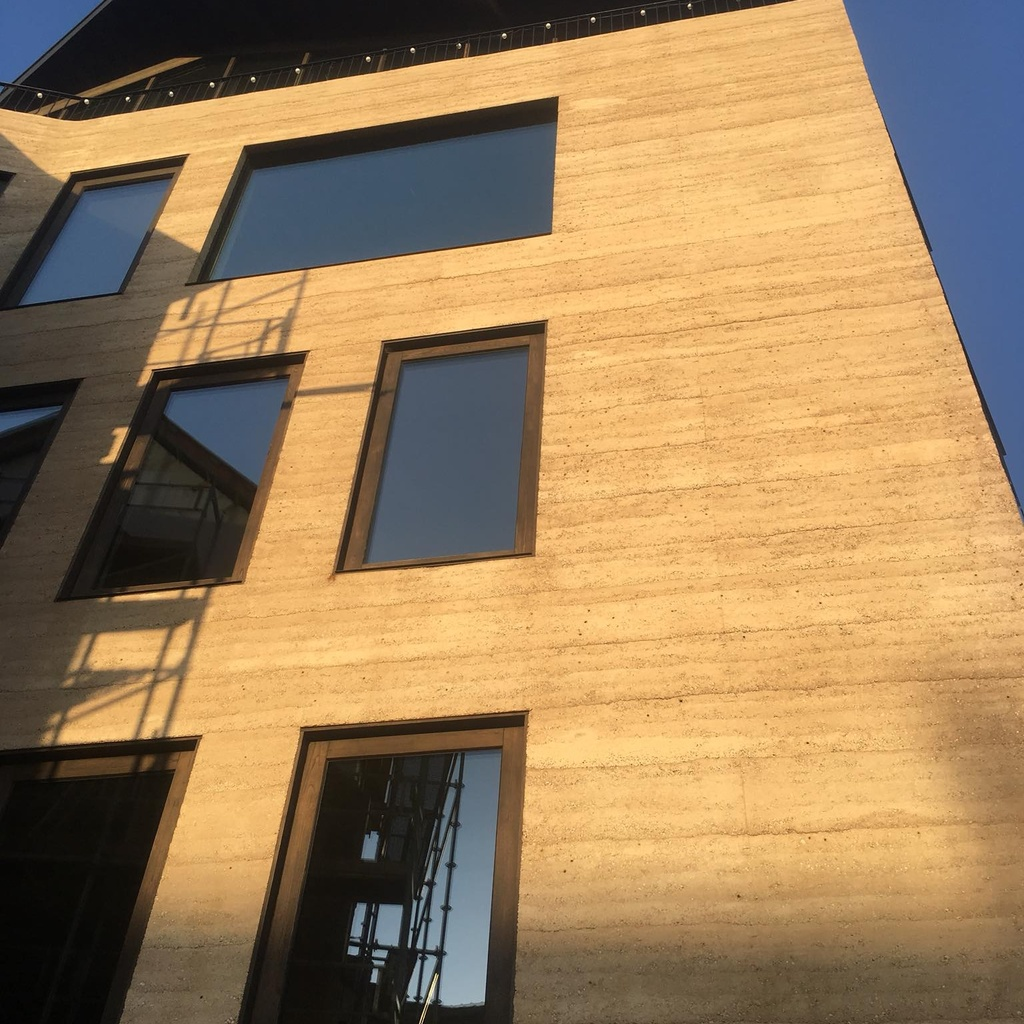
\includegraphics[width=\linewidth]{Images/LoRAs/STAMPBETON/Training_images/5.jpg} \\[2pt]

      % Row 2: images 6–10
      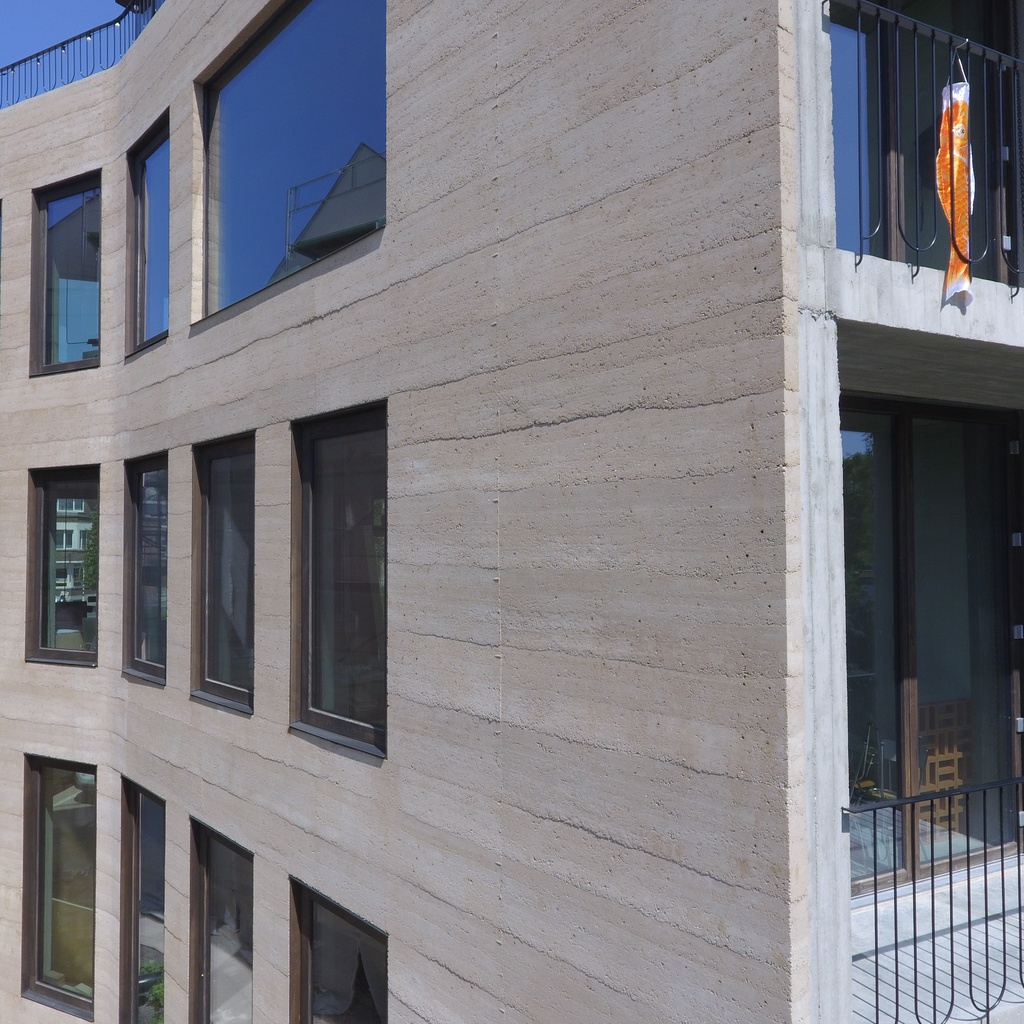
\includegraphics[width=\linewidth]{Images/LoRAs/STAMPBETON/Training_images/6.jpg} &
      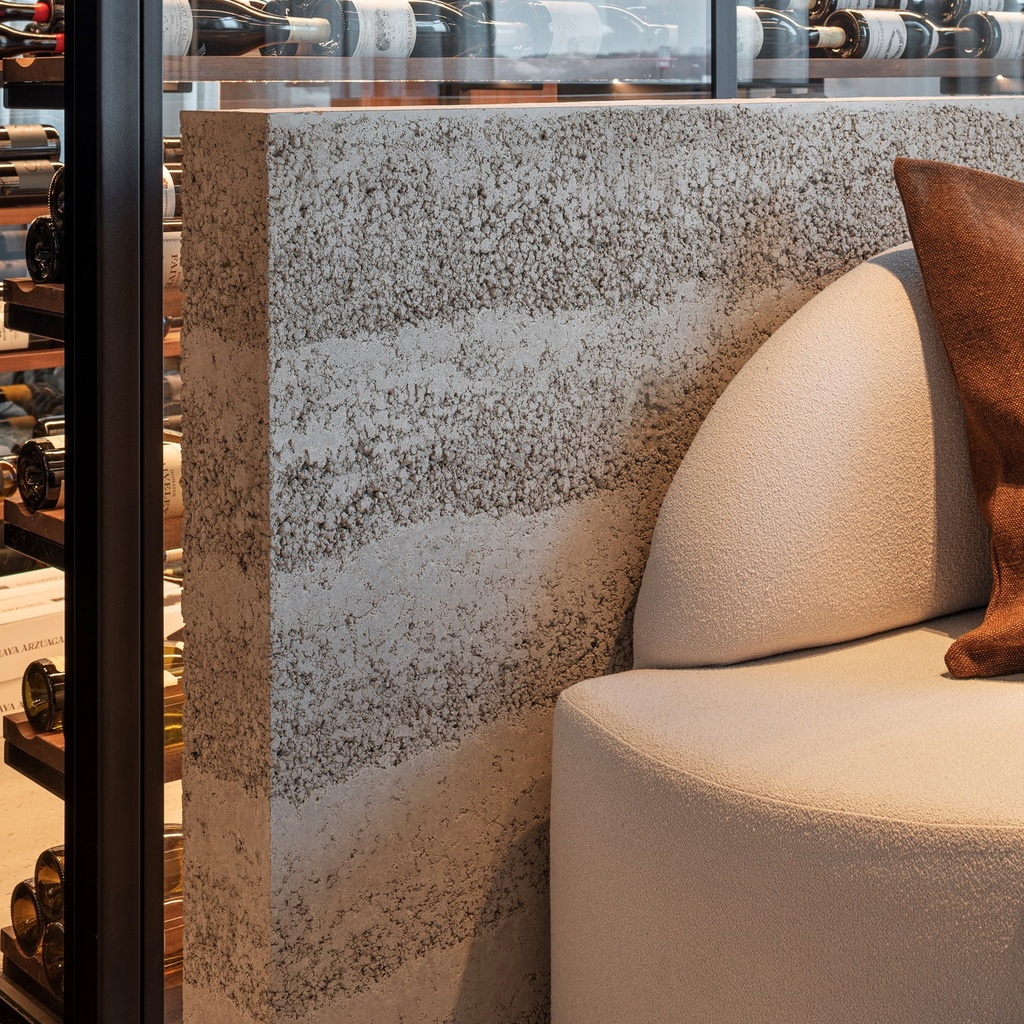
\includegraphics[width=\linewidth]{Images/LoRAs/STAMPBETON/Training_images/7.jpg} &
      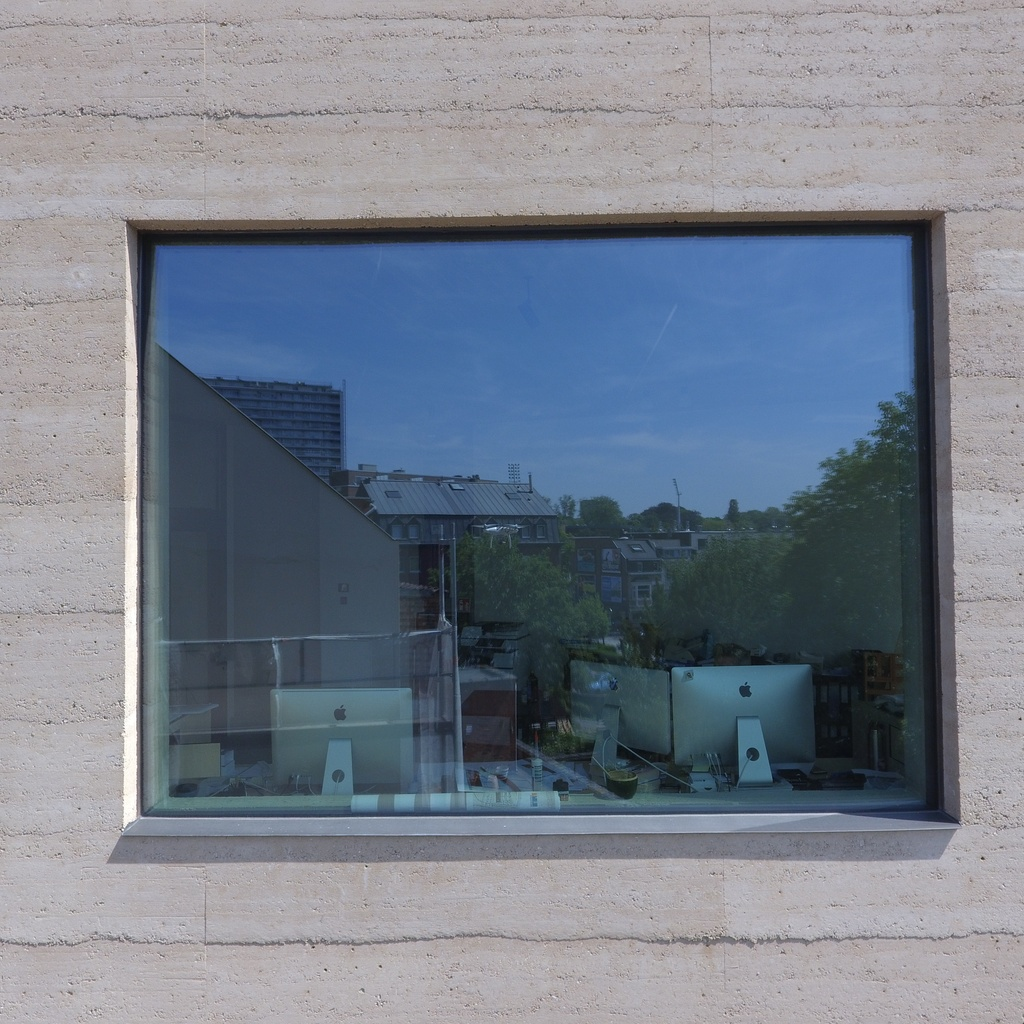
\includegraphics[width=\linewidth]{Images/LoRAs/STAMPBETON/Training_images/8.jpg} &
      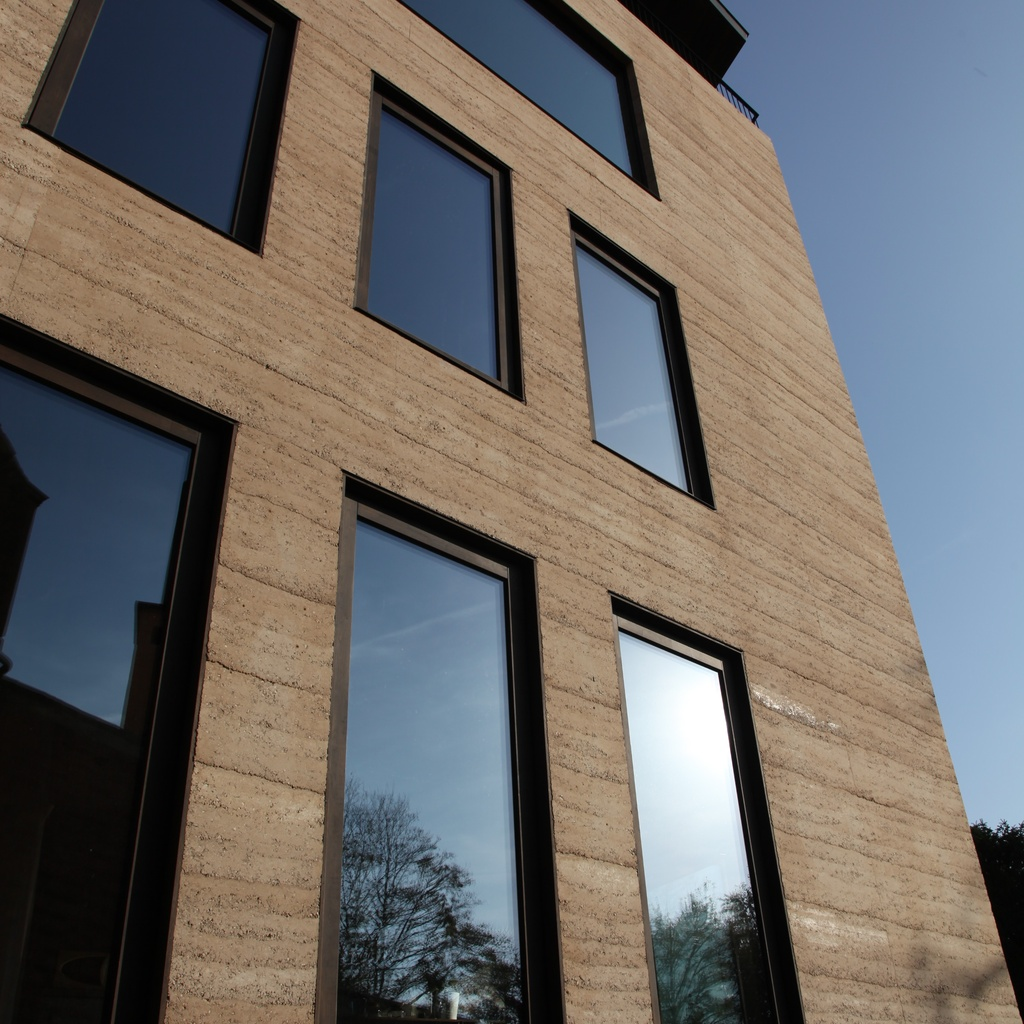
\includegraphics[width=\linewidth]{Images/LoRAs/STAMPBETON/Training_images/9.jpg} &
      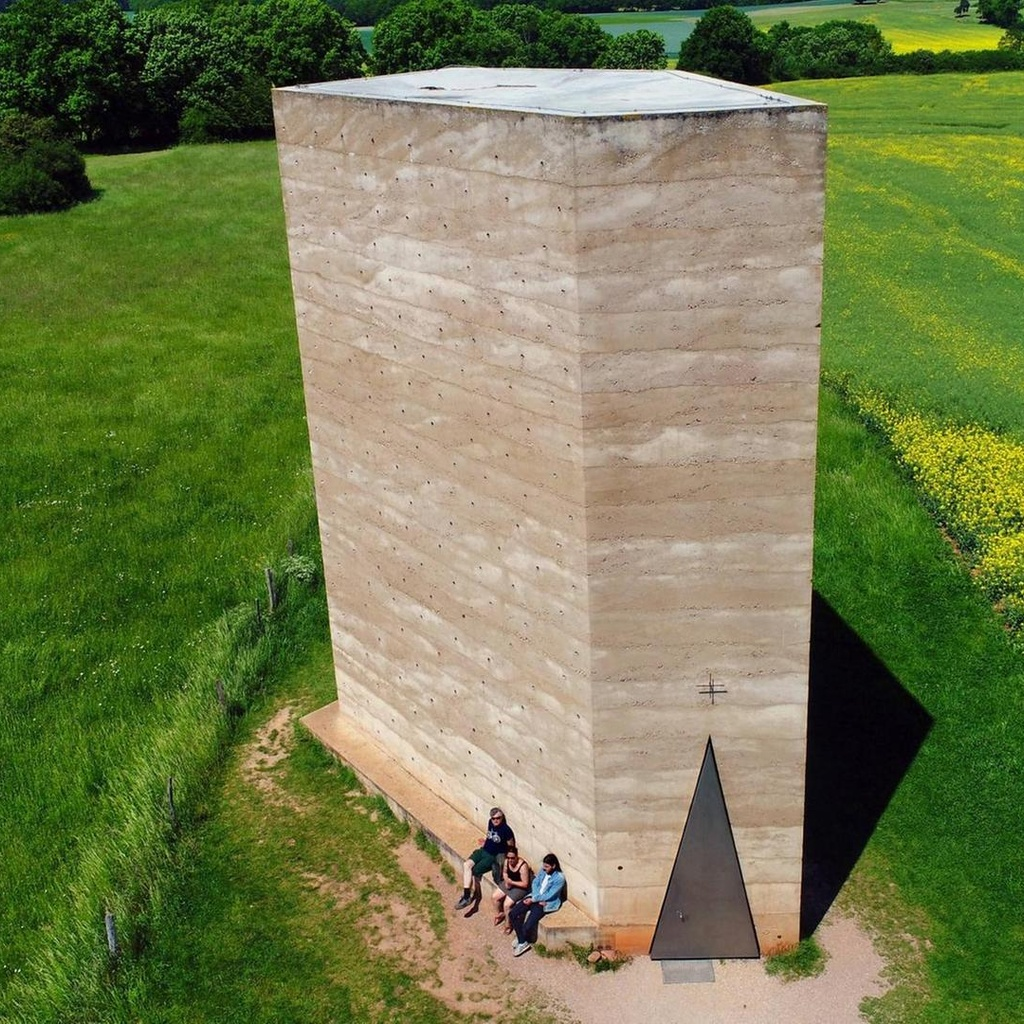
\includegraphics[width=\linewidth]{Images/LoRAs/STAMPBETON/Training_images/10.jpg} \\[2pt]

      % Row 3: images 11–15
      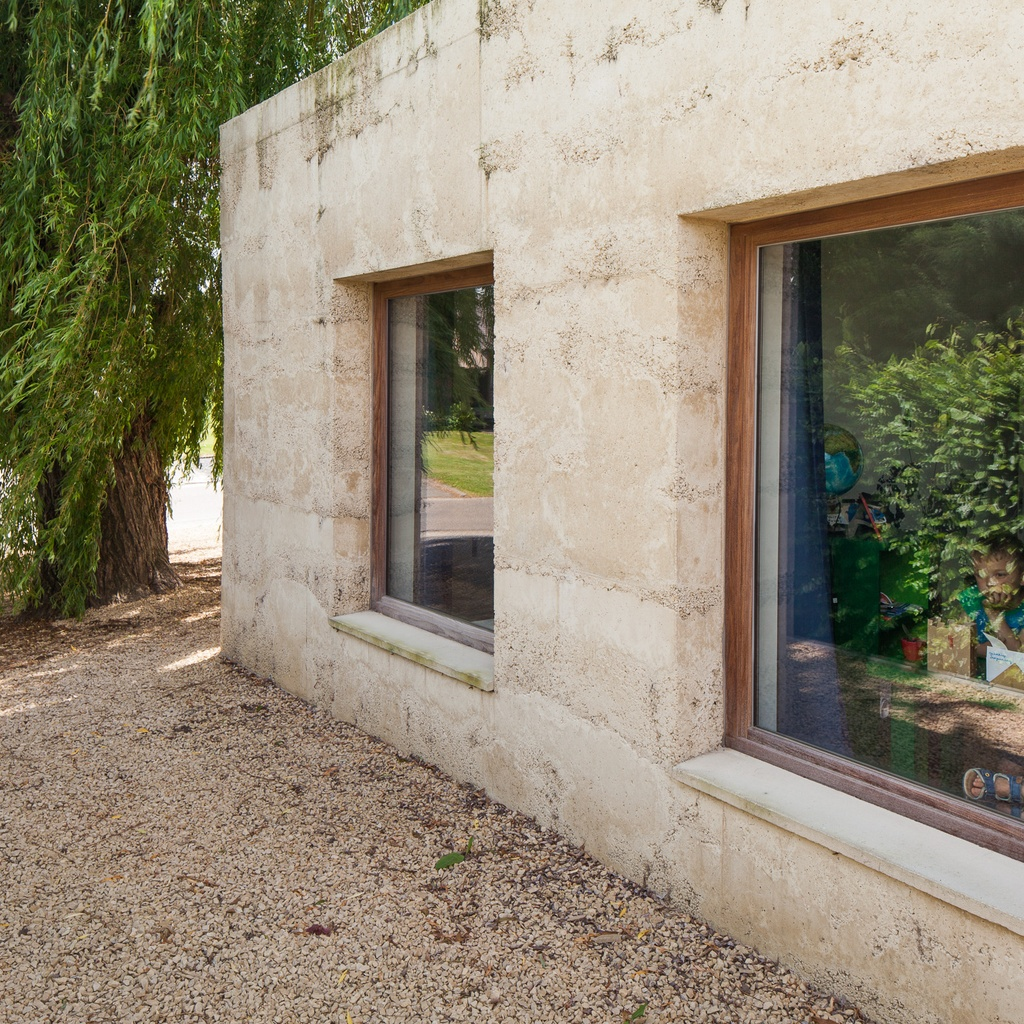
\includegraphics[width=\linewidth]{Images/LoRAs/STAMPBETON/Training_images/11.jpg} &
      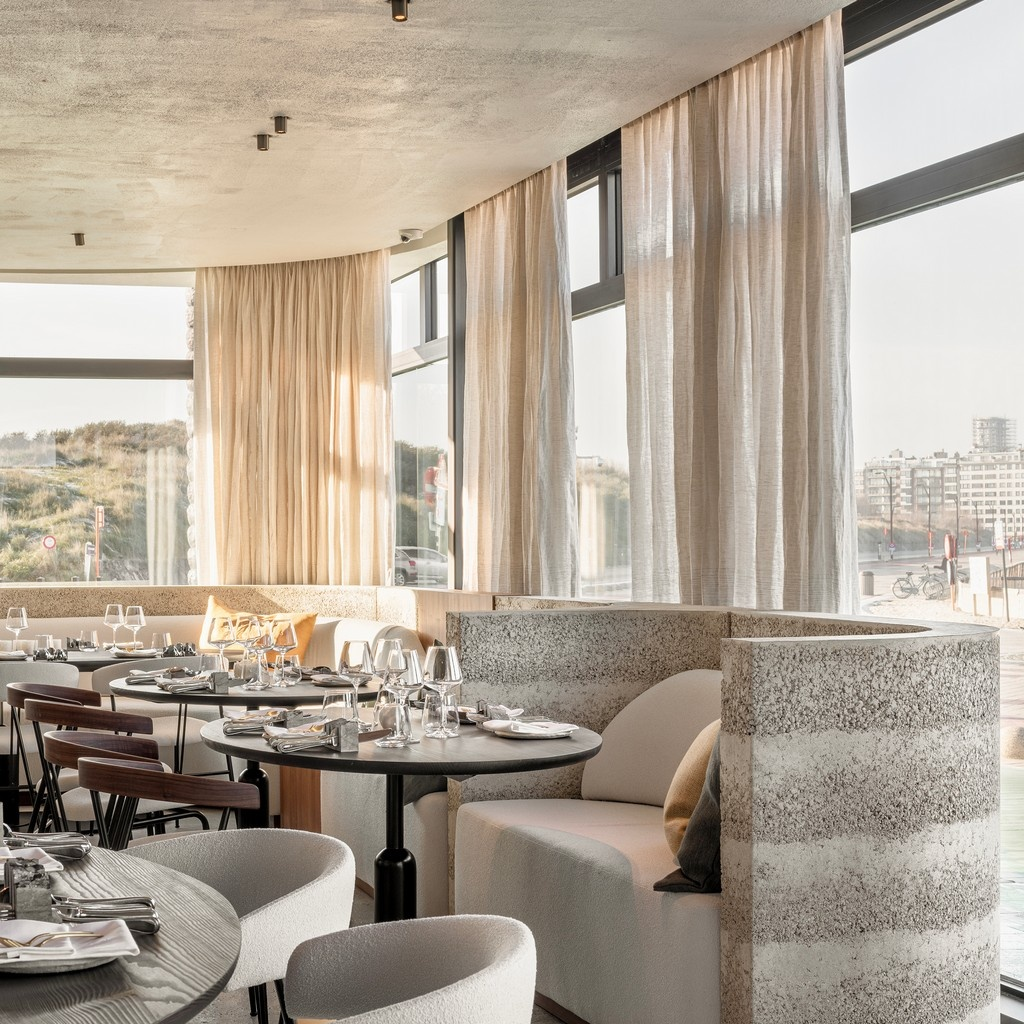
\includegraphics[width=\linewidth]{Images/LoRAs/STAMPBETON/Training_images/12.jpg} &
      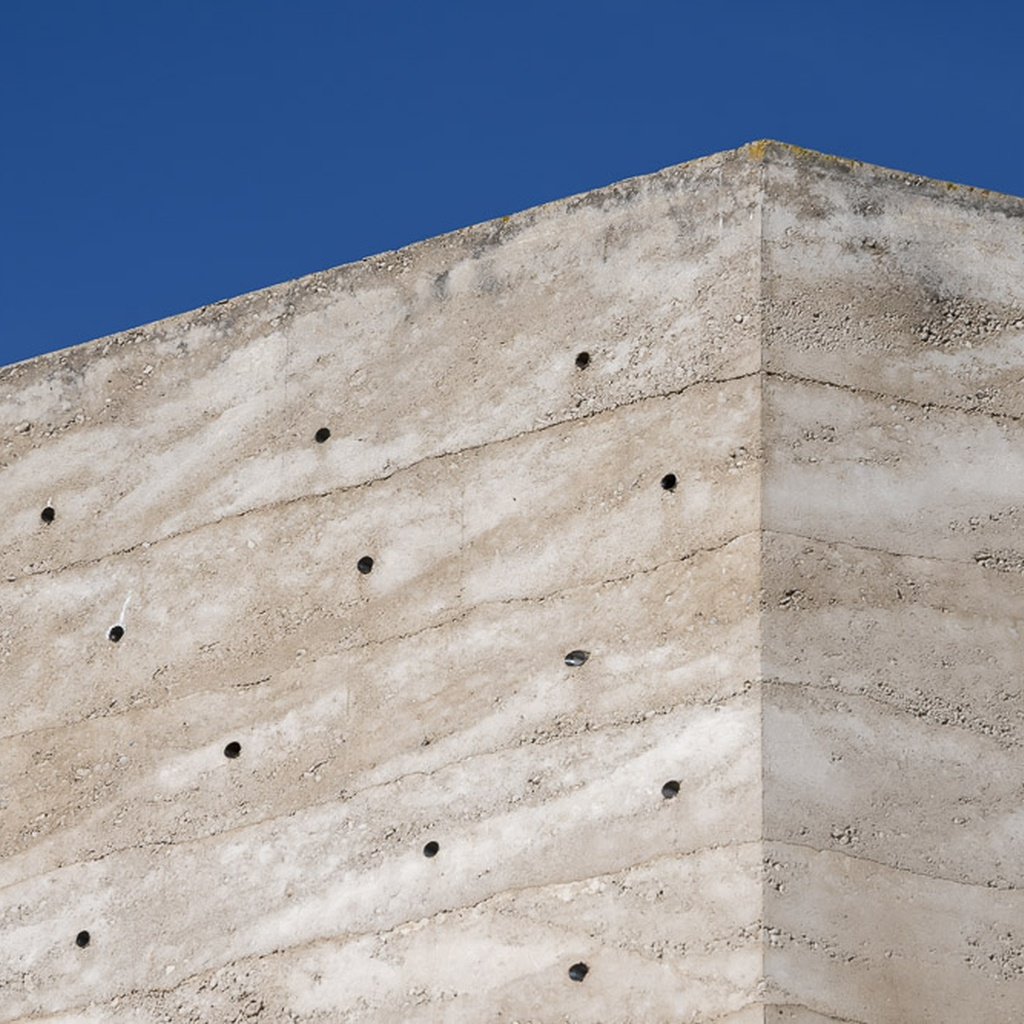
\includegraphics[width=\linewidth]{Images/LoRAs/STAMPBETON/Training_images/13.jpg} &
      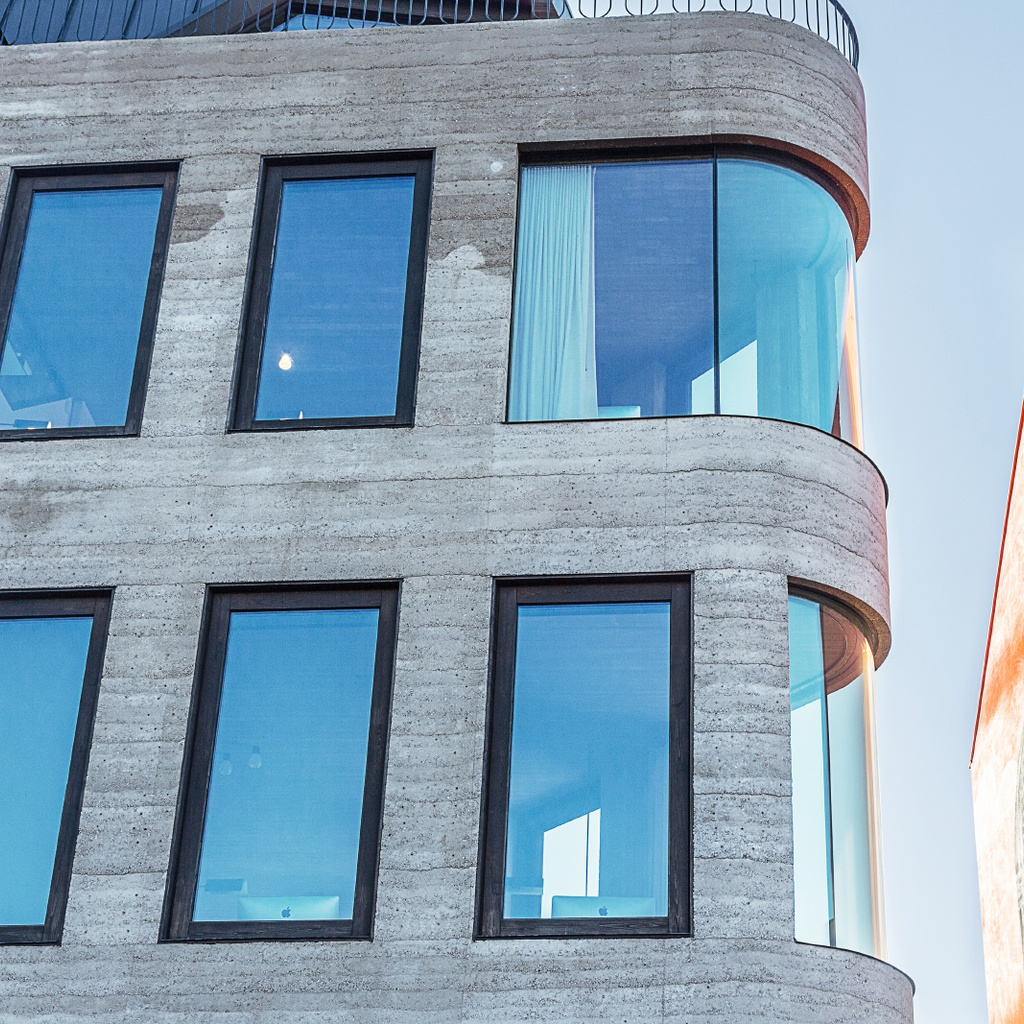
\includegraphics[width=\linewidth]{Images/LoRAs/STAMPBETON/Training_images/14.jpg} &
      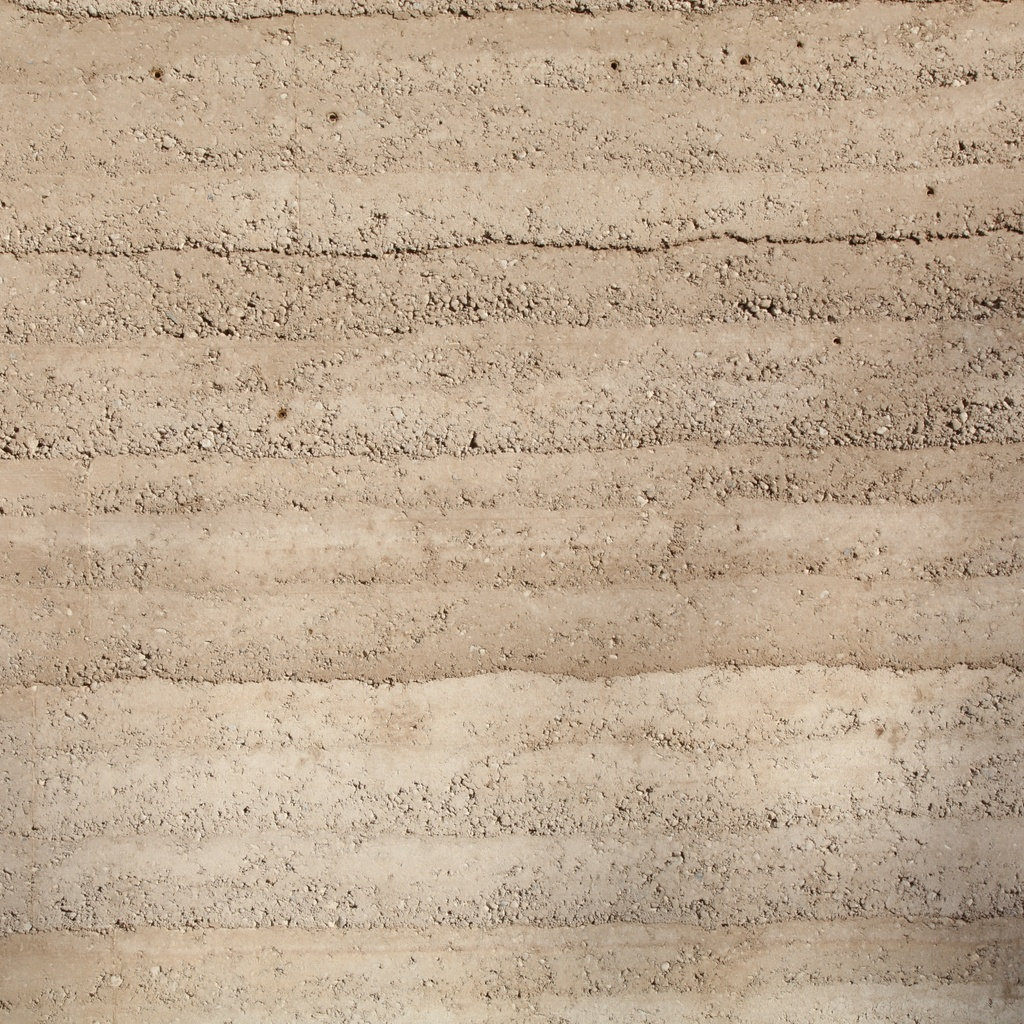
\includegraphics[width=\linewidth]{Images/LoRAs/STAMPBETON/Training_images/15.jpg} \\
    \end{tabular}
  }
  \caption{The images used to train the stampbeton LoRA.}
  \label{fig:gridstampbeton}
\end{figure}

% Upon the first training, the model seemed to be 'undertrained': in some images, there were vertical lines on the material and they were not properly captioned, so the model incorporated that into its idea of the material.\\
% \begin{figure}[H]
%     \centering
%     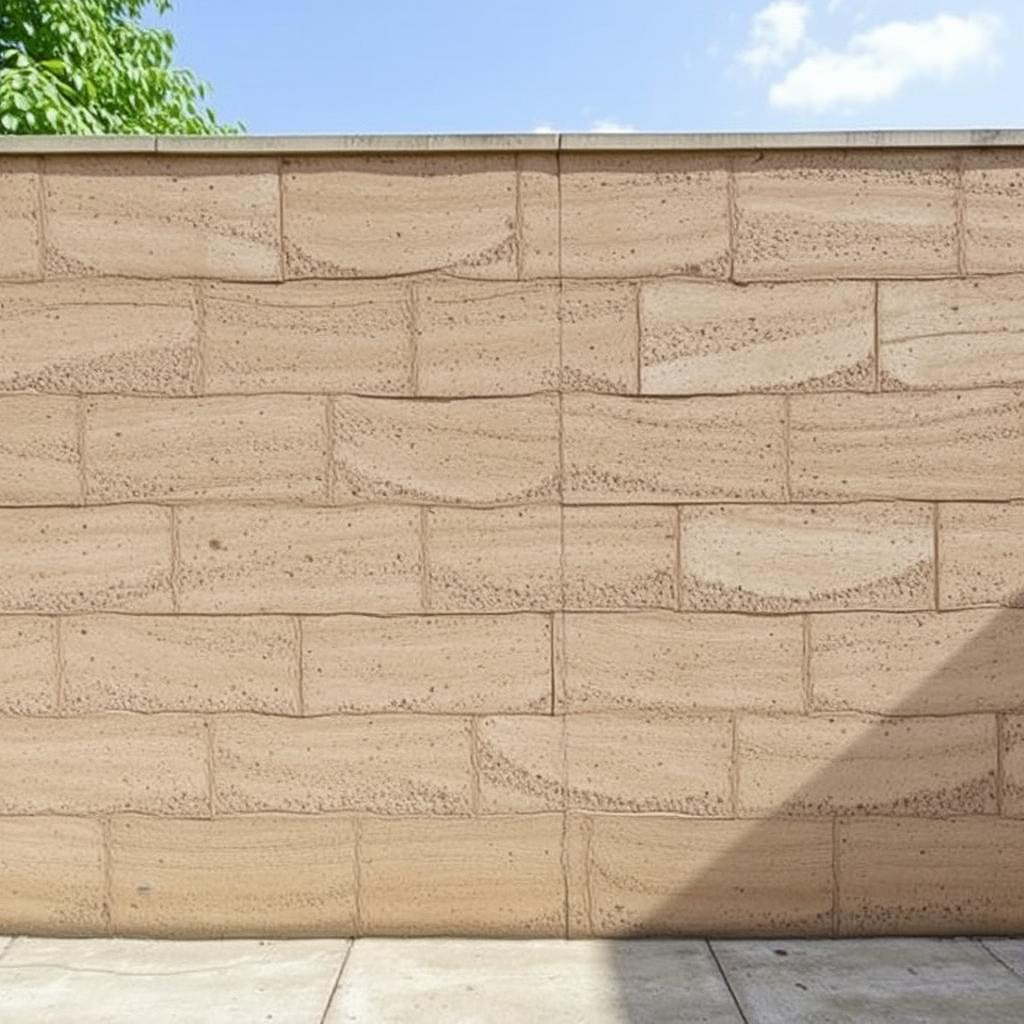
\includegraphics[width=0.5\linewidth]{afbeeldingen/STAMPBETON/v1 .png}
%     \caption{An image produced with the first stampbeton LoRA, showcasing the masonry-like texture caused by overfitting. Prompt: 'Stampbeton wall with bold horizontal strata'.}
%     \label{fig:stampbeton v1}
% \end{figure}
% For the second version, the captions were modified and this problem was, largely, resolved. The model did not give perfect images of stamped concrete 100\% of the time; sometimes, the masonry structure would pop up again, but way less than with version 1. 
% \begin{figure}[H]
%     \centering
%     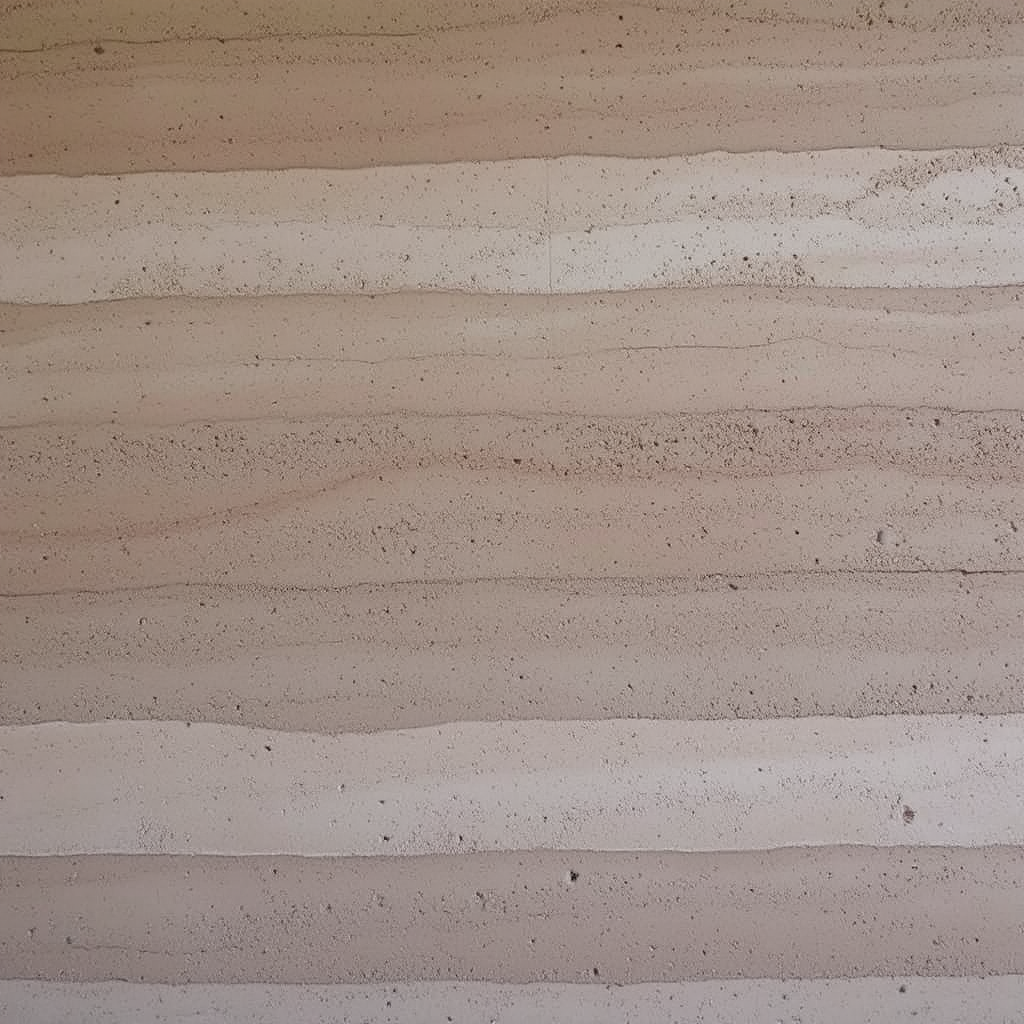
\includegraphics[width=0.5\linewidth]{afbeeldingen/STAMPBETON/v2.png}
%     \caption{An image produced with the second stampbeton LoRA, showing the structure that the model understands to be stamped concrete. Prompt: 'Stampbeton wall with bold horizontal strata'.}
%     \label{fig:stampbeton v2}
% \end{figure}

\subsubsection{3D-effect}
The second LoRA creates a 3D-effect in facades, which is obtained by adding protruding elements to the facade, such as a tent or a canopy. The purpose of creating a 3D-effect is to make the facade feel more warm inviting.\\
After validation, one image (figure \ref{fig:3deffectomittedimage}) was left out of the original dataset: the image did not suit the design-oriented preferences of the architect.
\begin{figure}[H]
    \centering
    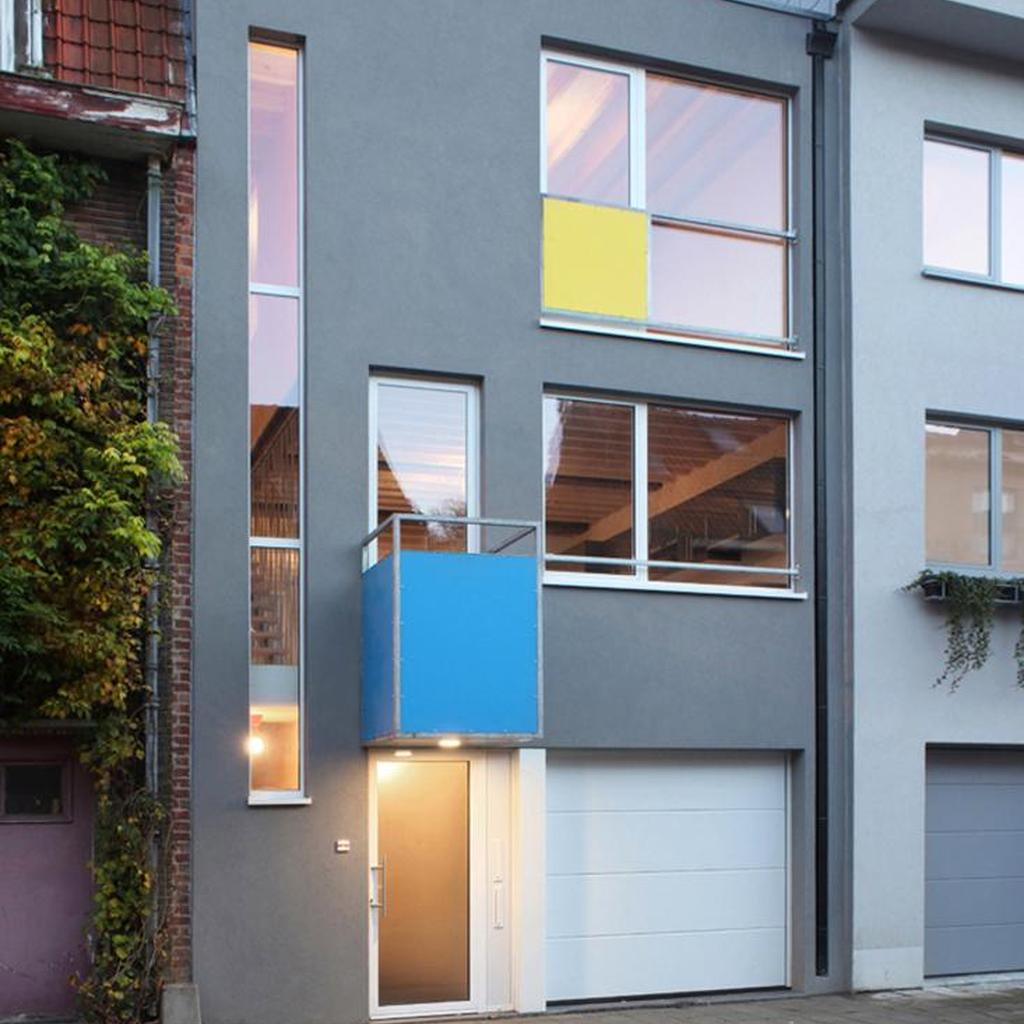
\includegraphics[width=0.24\linewidth]{Images//LoRAs//3D-effect/4.jpg}
    \caption{The image removed from the original 3D-effect dataset.}
    \label{fig:3deffectomittedimage}
\end{figure}
Figure \ref{fig:grid3D-effect} portrays the training images for this LoRA.
\begin{figure}[H]
  \centering
  \resizebox{\textwidth}{!}{%
    \begin{tabular}{@{}ccccc@{}}
      % Row 1: images 1–5
      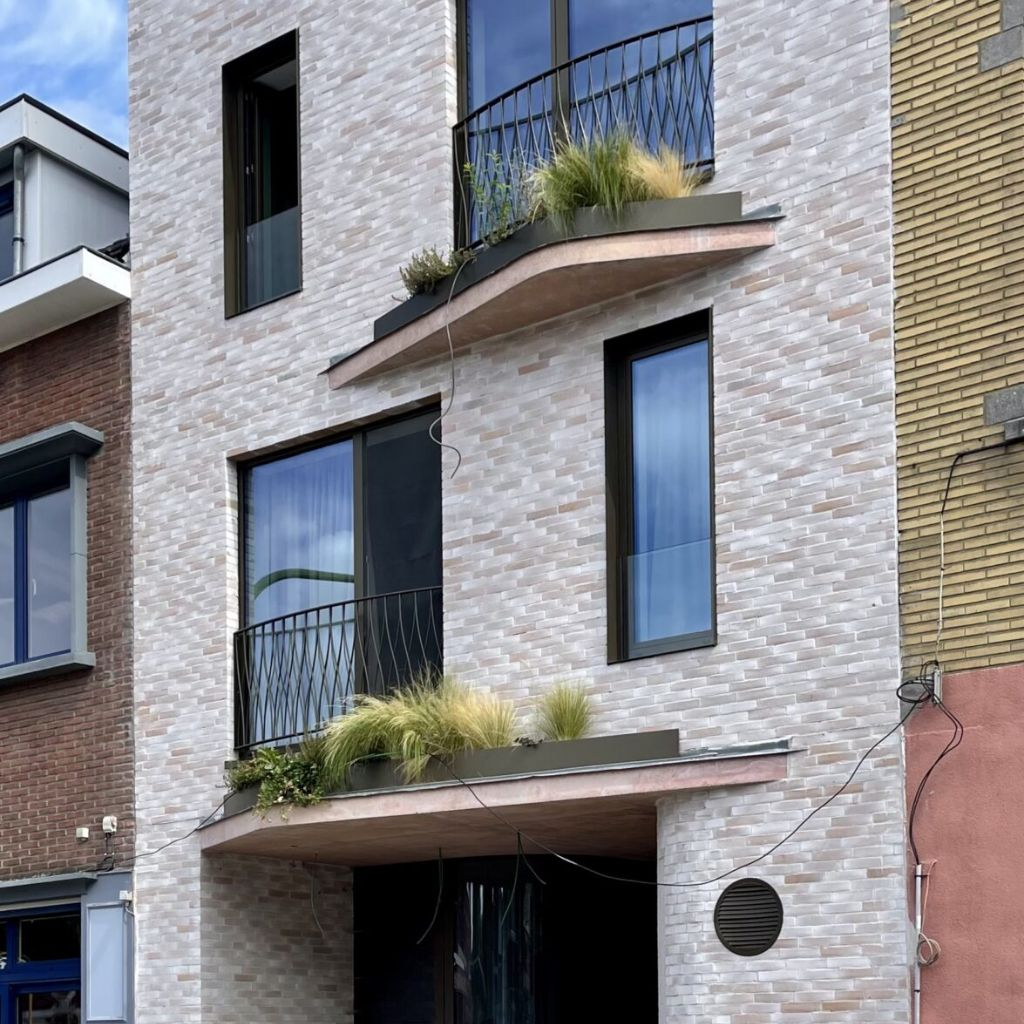
\includegraphics[width=\linewidth]{Images/LoRAs/3D-effect/Training_images/1.jpeg} &
      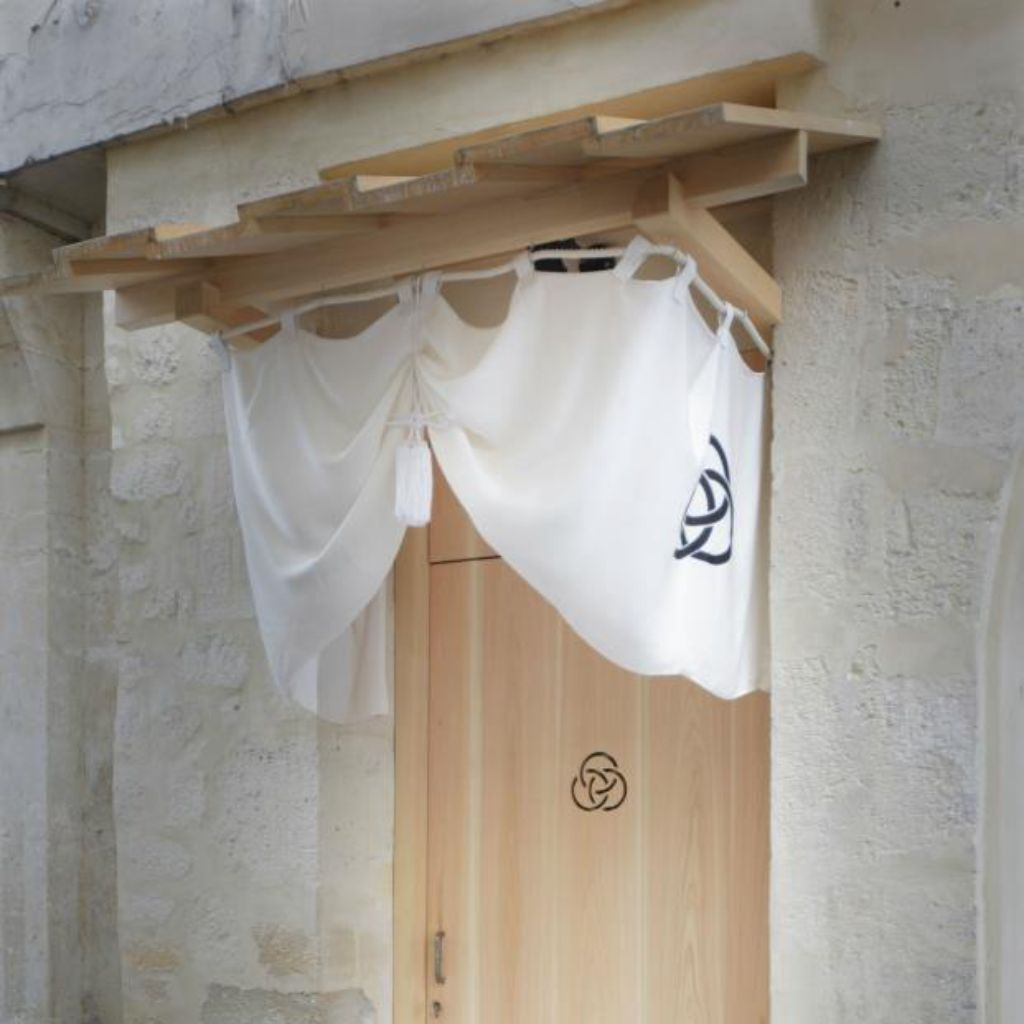
\includegraphics[width=\linewidth]{Images/LoRAs/3D-effect/Training_images/2.jpg} &
      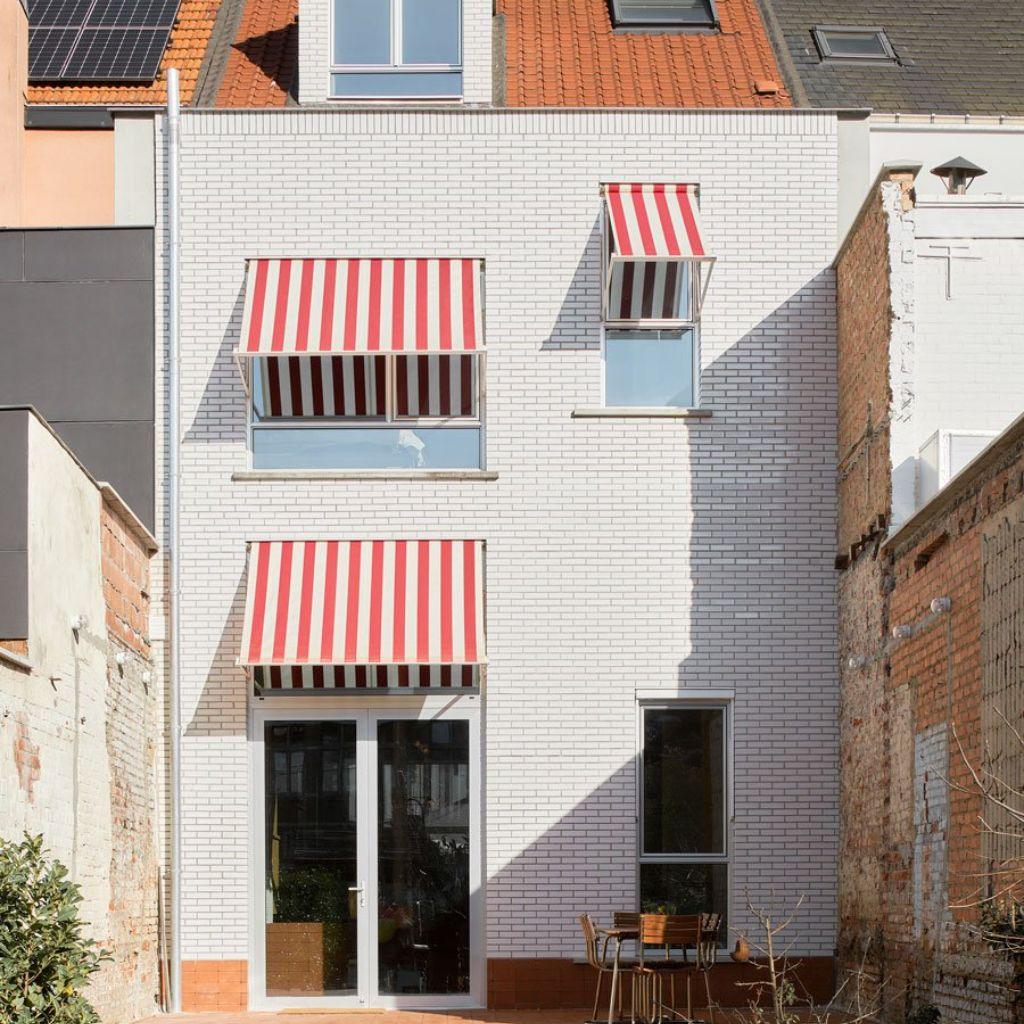
\includegraphics[width=\linewidth]{Images/LoRAs/3D-effect/Training_images/3.jpg} &
      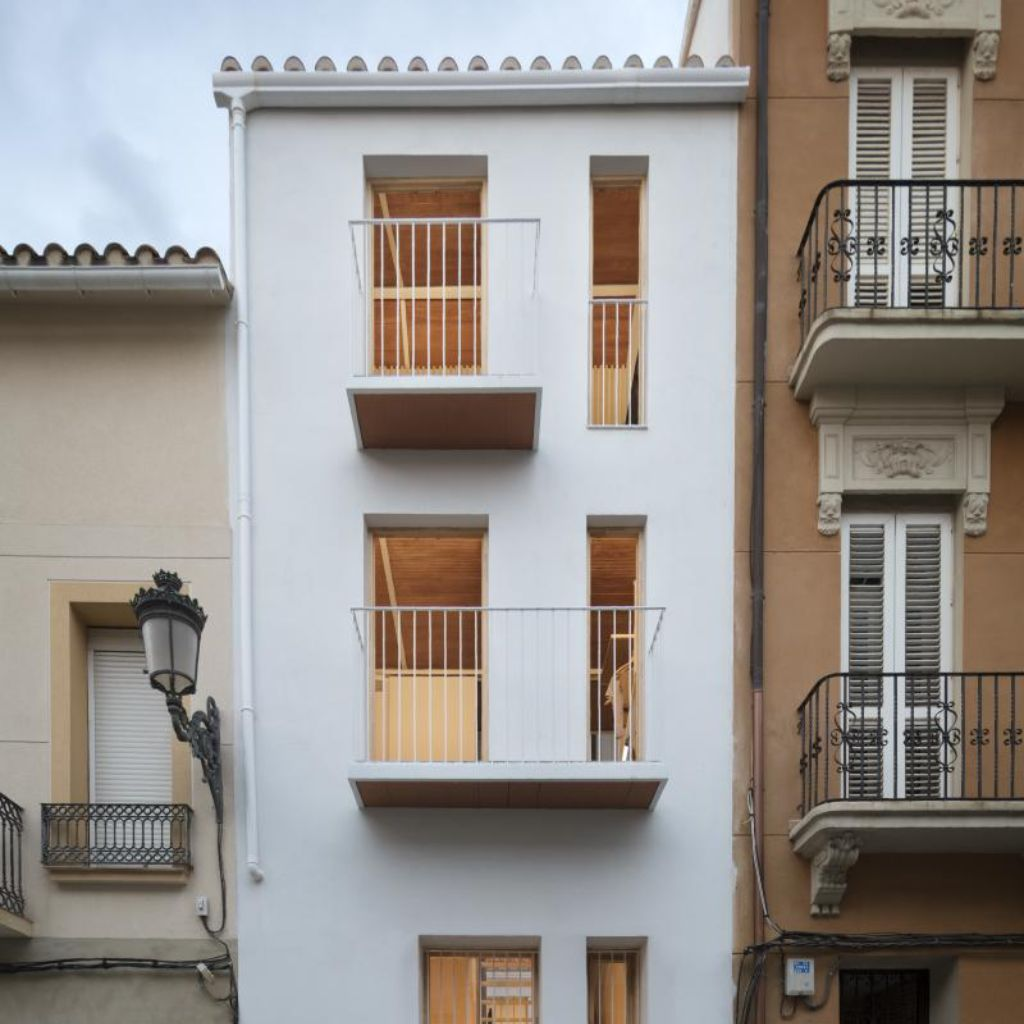
\includegraphics[width=\linewidth]{Images/LoRAs/3D-effect/Training_images/4.jpg} &
      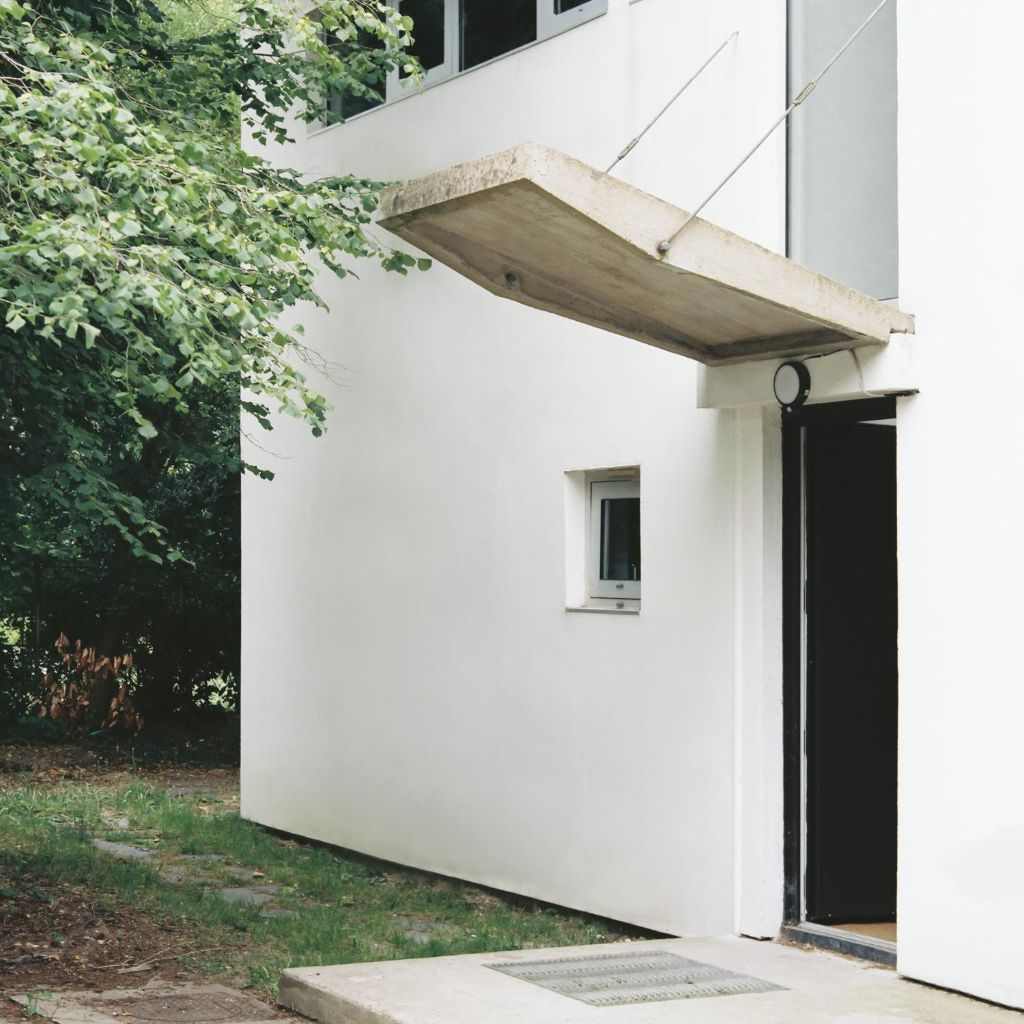
\includegraphics[width=\linewidth]{Images/LoRAs/3D-effect/Training_images/5.jpg} \\[2pt]

      % Row 2: images 6–10
      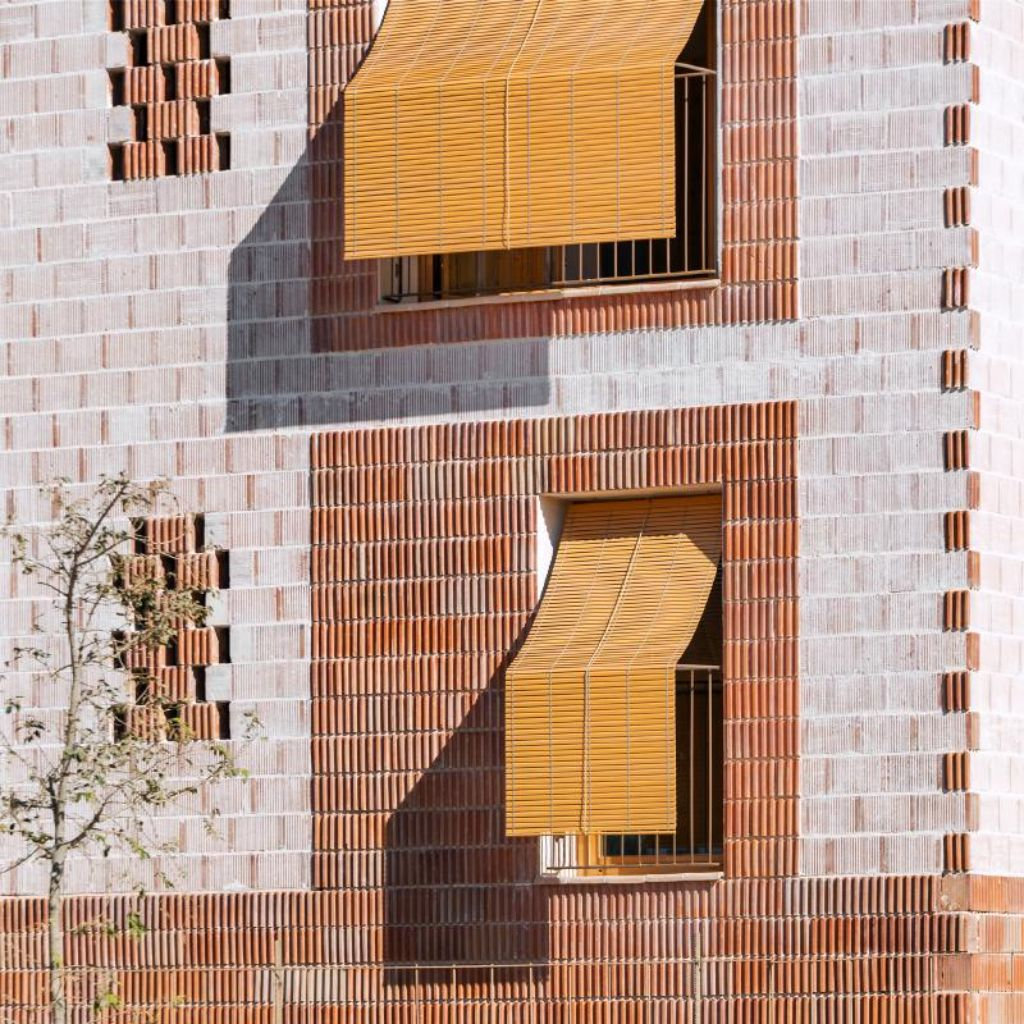
\includegraphics[width=\linewidth]{Images/LoRAs/3D-effect/Training_images/6.jpg} &
      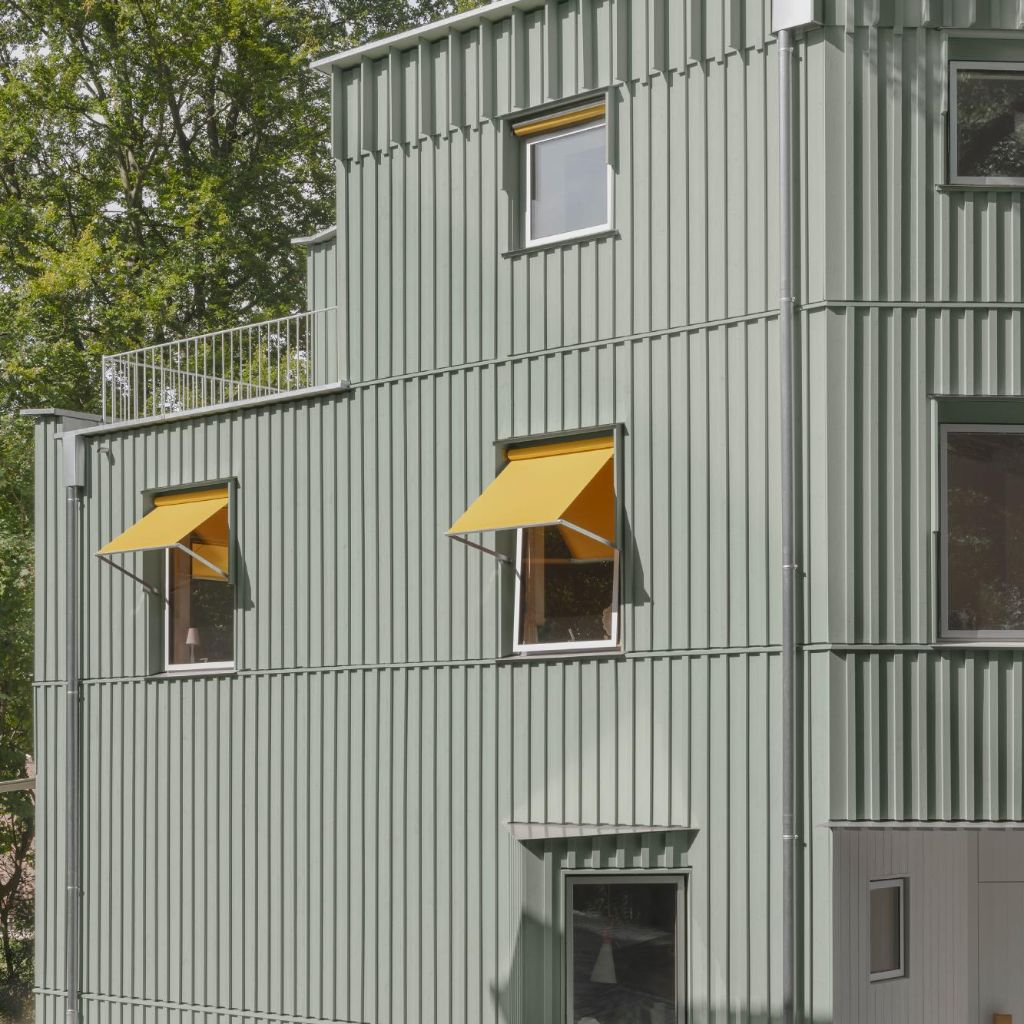
\includegraphics[width=\linewidth]{Images/LoRAs/3D-effect/Training_images/7.jpg} &
      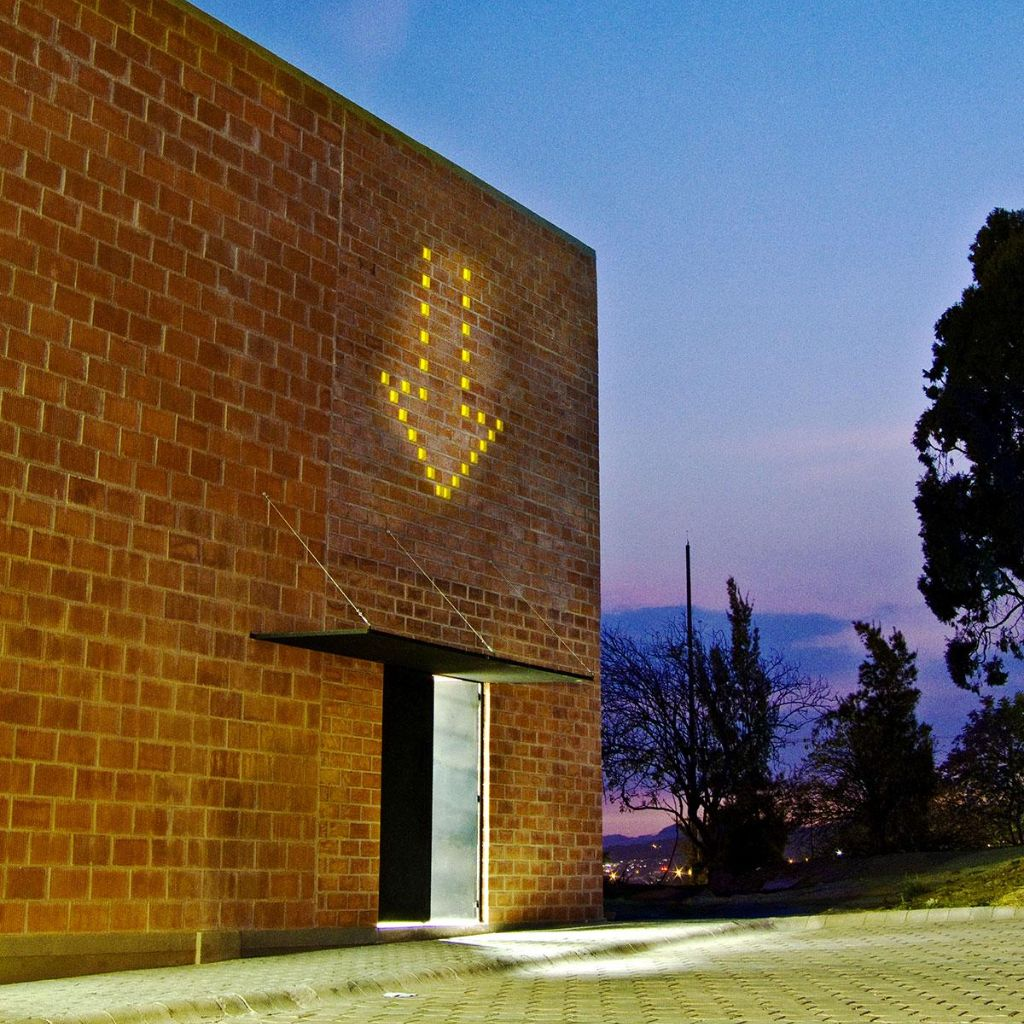
\includegraphics[width=\linewidth]{Images/LoRAs/3D-effect/Training_images/8.jpg} &
      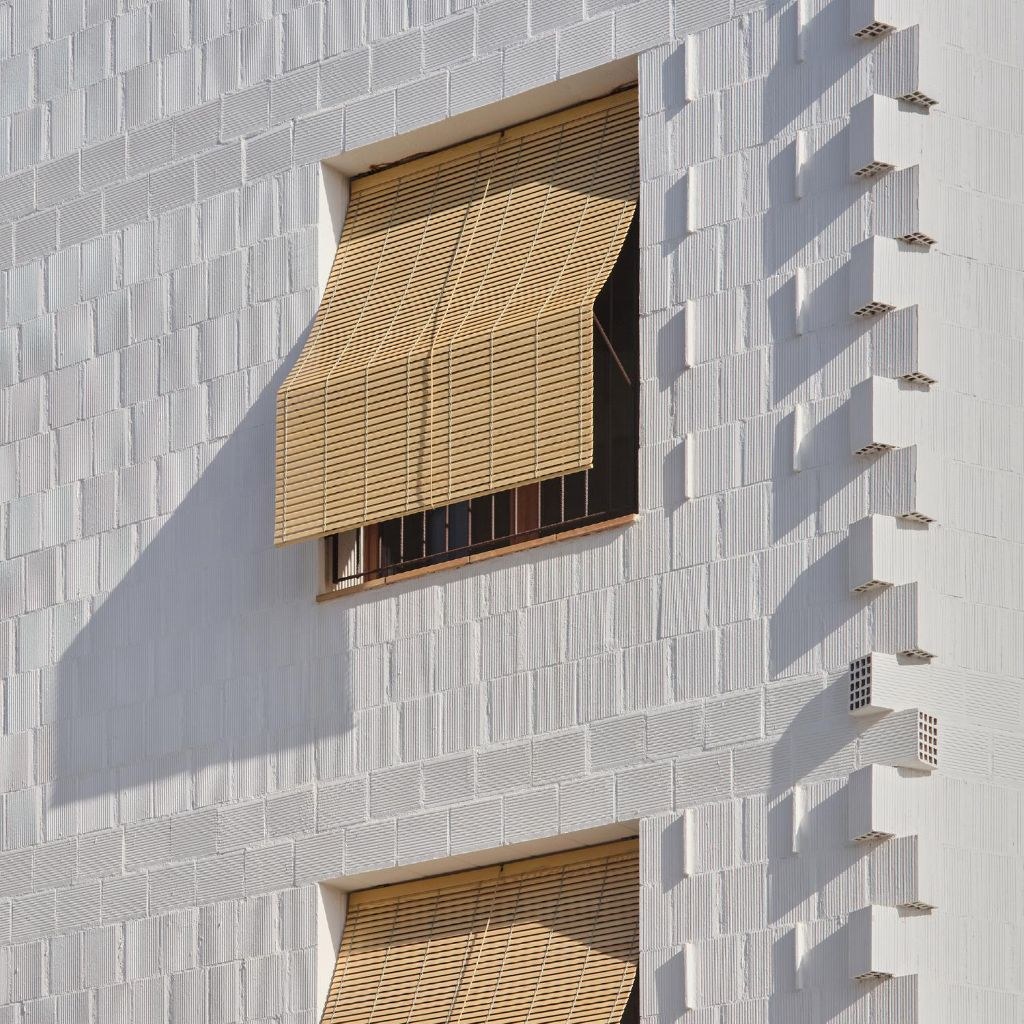
\includegraphics[width=\linewidth]{Images/LoRAs/3D-effect/Training_images/9.jpg} &
      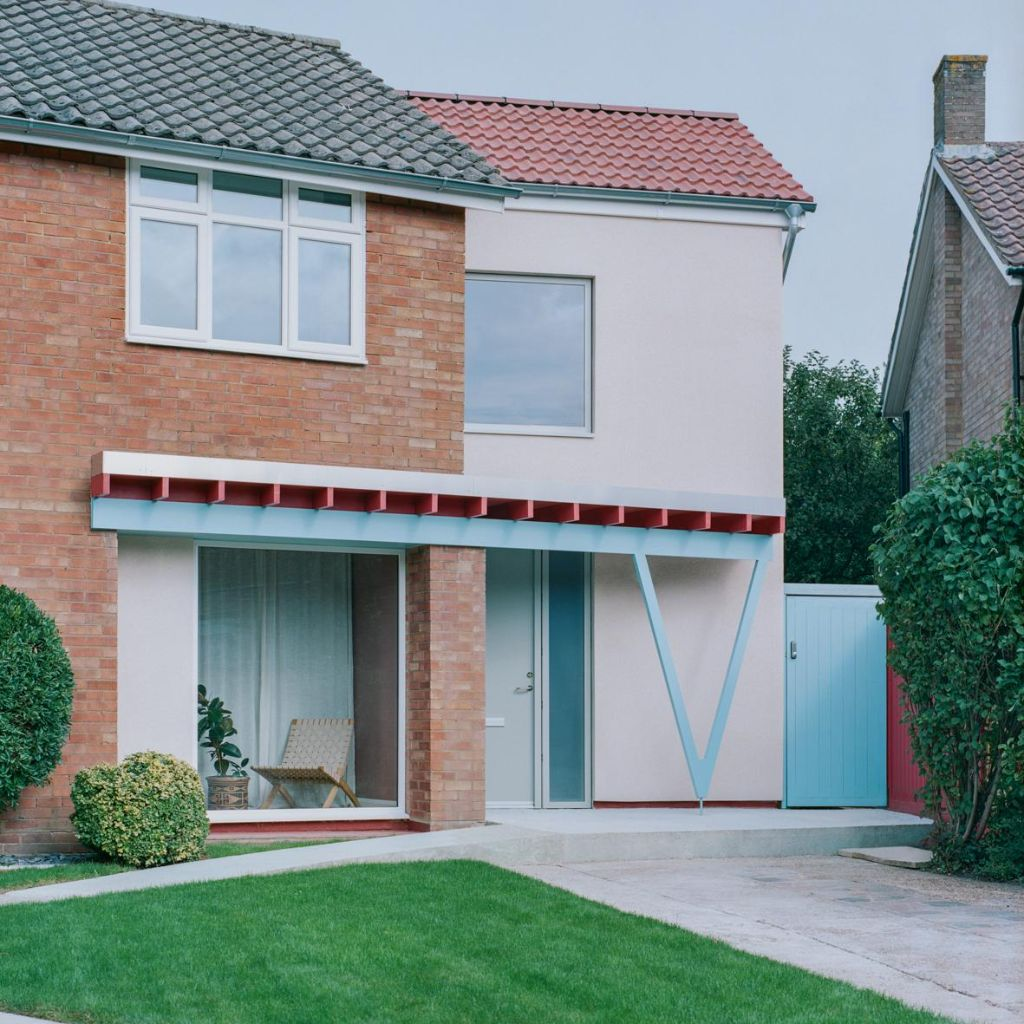
\includegraphics[width=\linewidth]{Images/LoRAs/3D-effect/Training_images/10.jpg} \\[2pt]

      % Row 3: images 11–15
      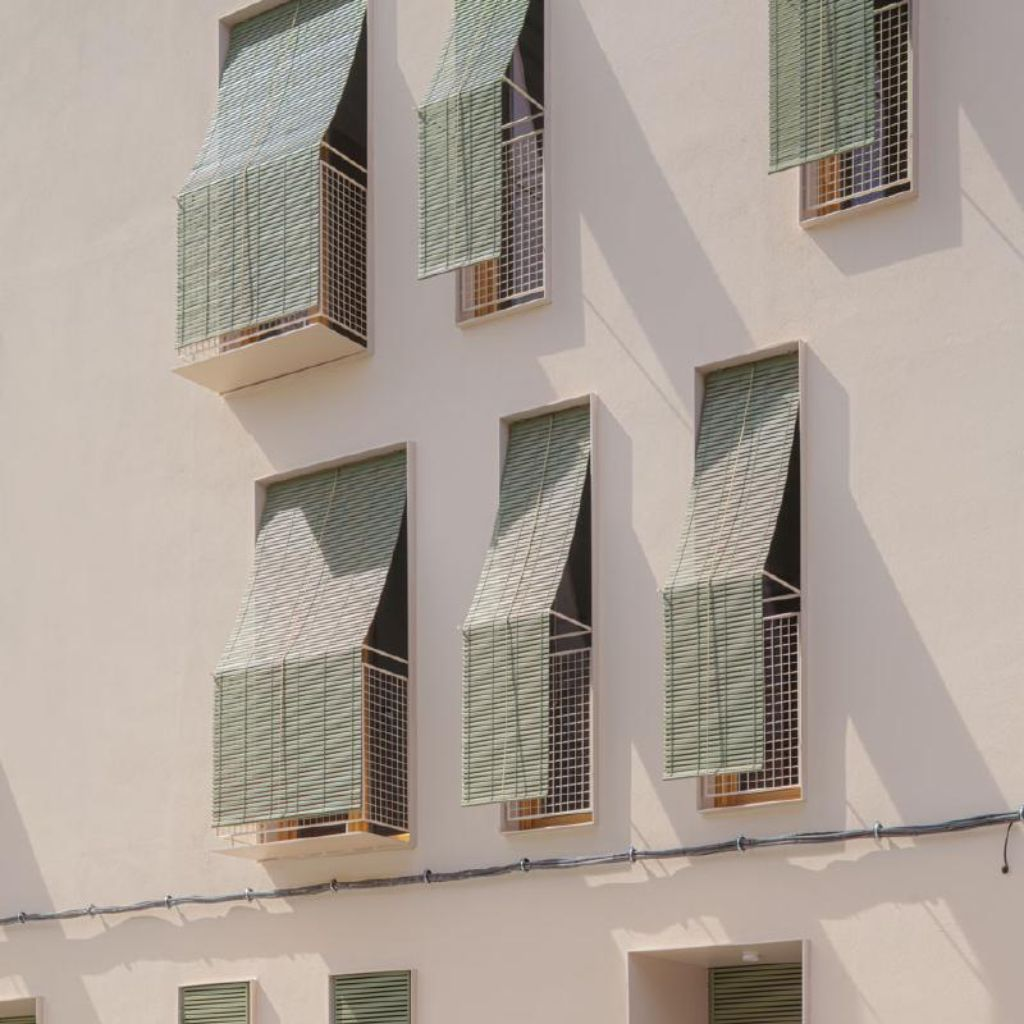
\includegraphics[width=\linewidth]{Images/LoRAs/3D-effect/Training_images/11.jpg} &
      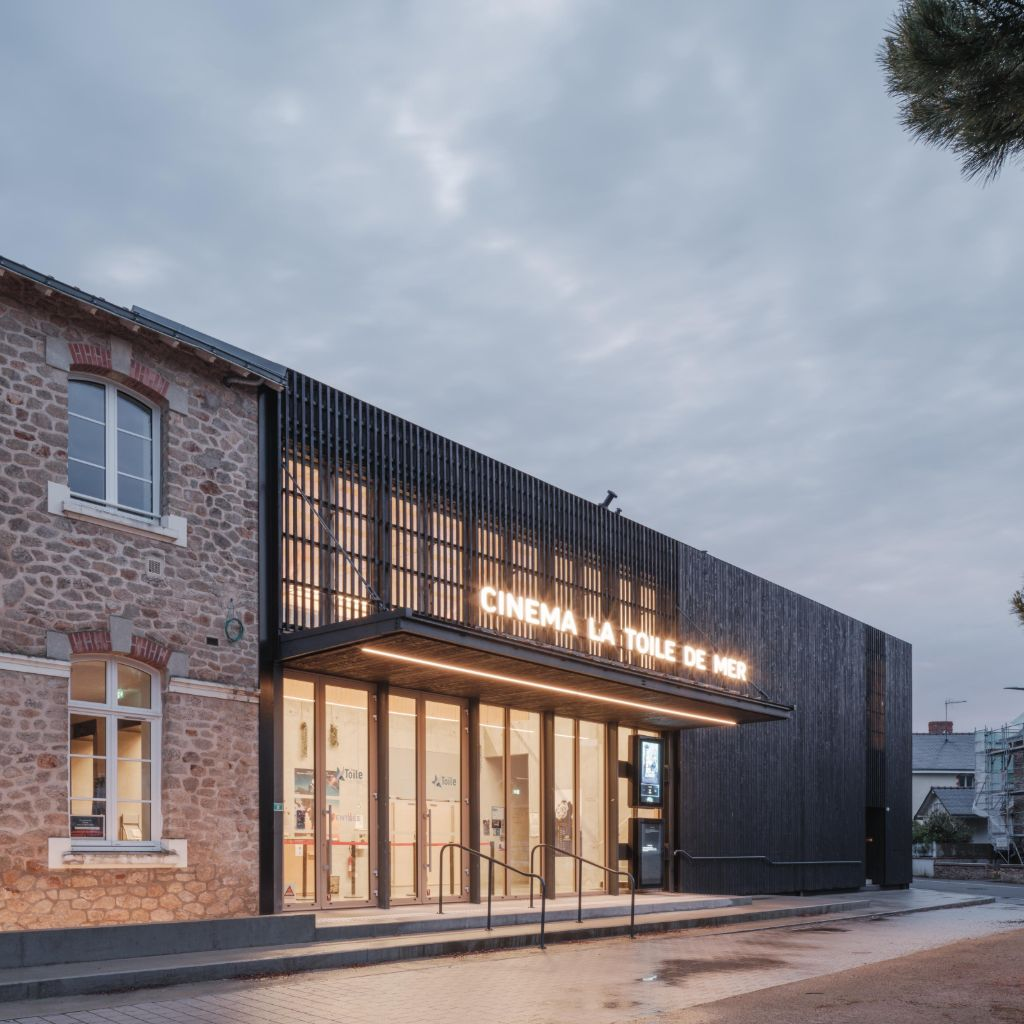
\includegraphics[width=\linewidth]{Images/LoRAs/3D-effect/Training_images/12.jpg} &
      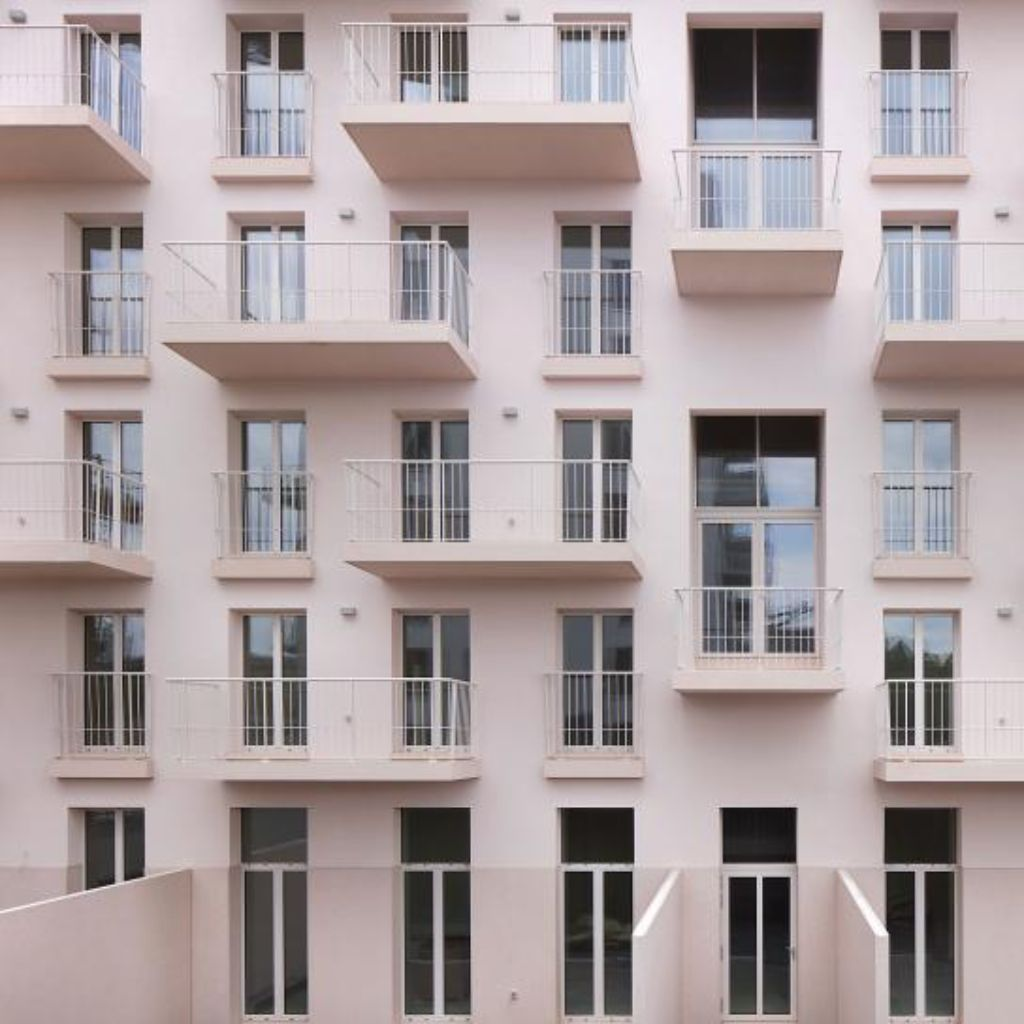
\includegraphics[width=\linewidth]{Images/LoRAs/3D-effect/Training_images/13.jpg} &
      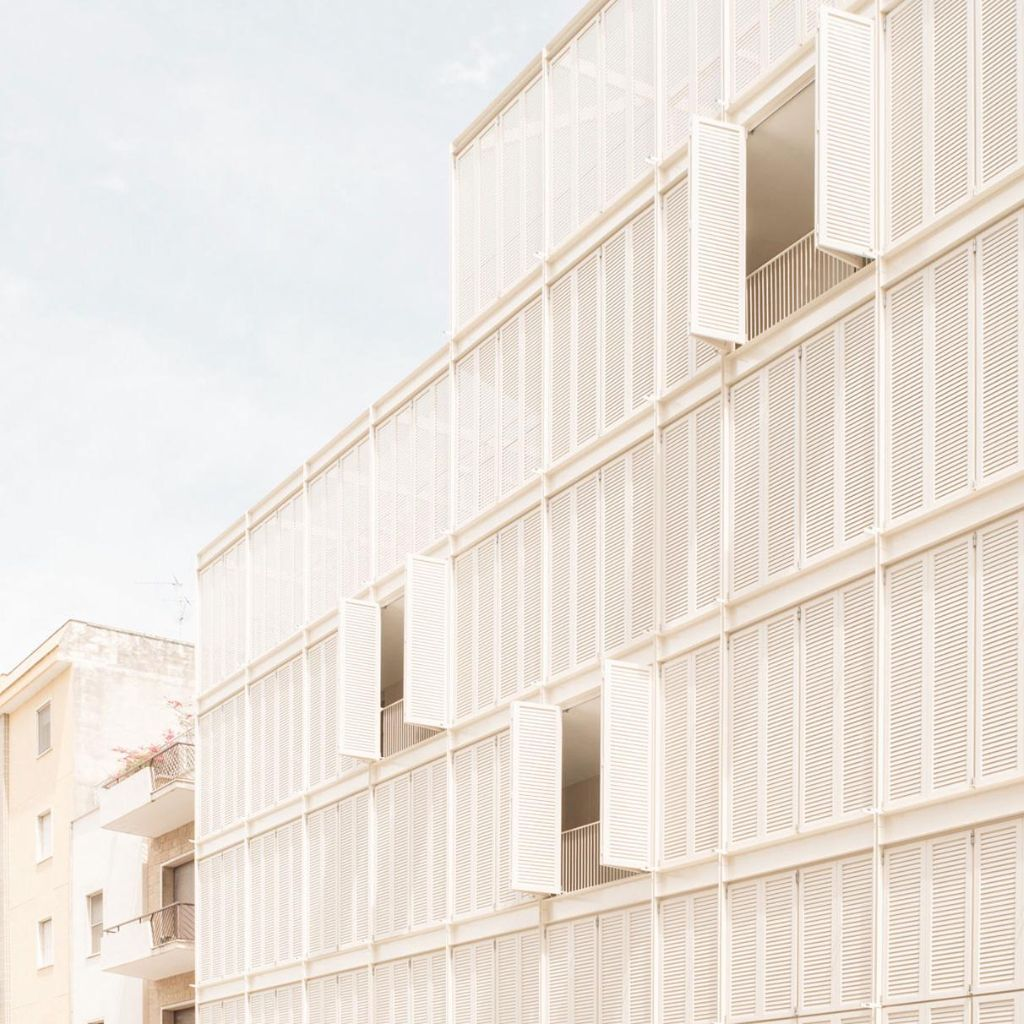
\includegraphics[width=\linewidth]{Images/LoRAs/3D-effect/Training_images/14.jpg} &
      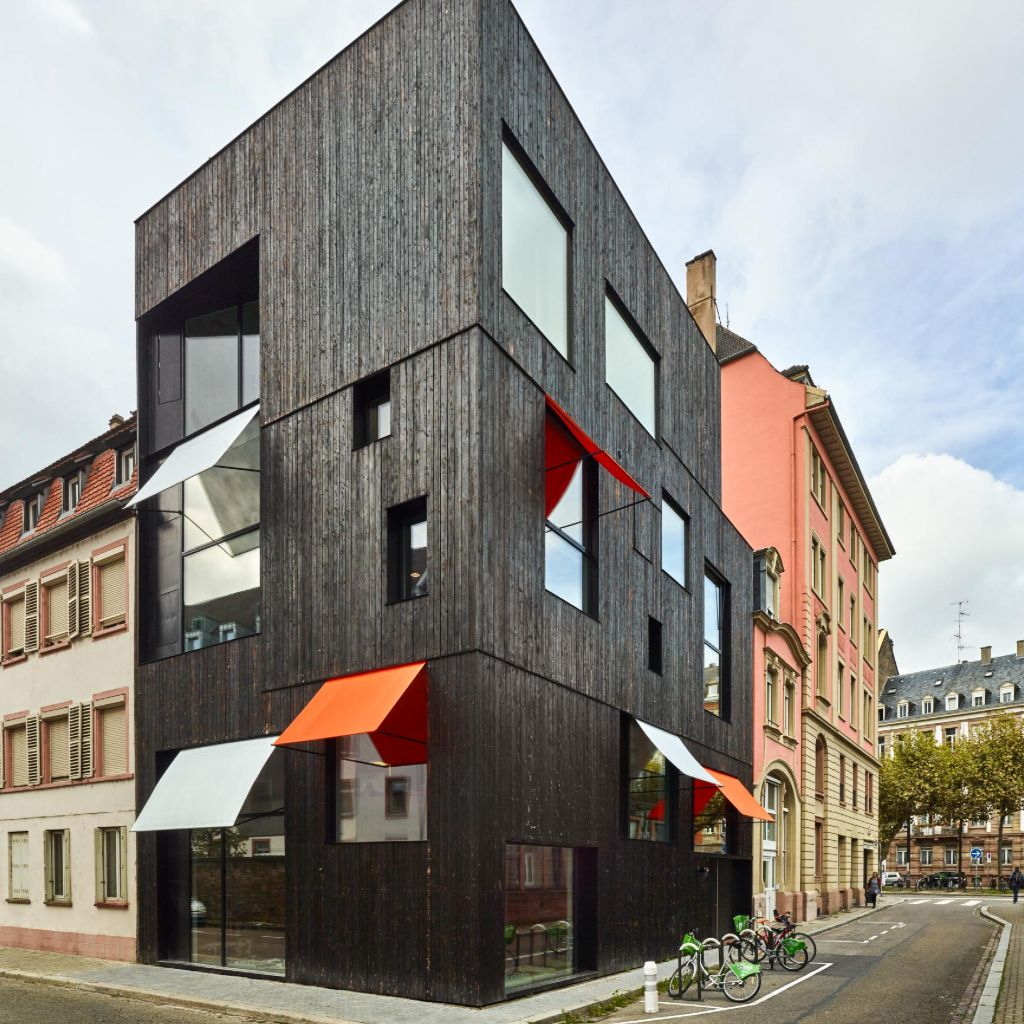
\includegraphics[width=\linewidth]{Images/LoRAs/3D-effect/Training_images/15.jpg} \\
    \end{tabular}%
  }
  \caption{The images used to train the 3D-effect LoRA.}
  \label{fig:grid3D-effect}
\end{figure}

\subsubsection{Geleding}
The third and last LoRA for DMOA replicates the concept of dividing two floors from each other in the facade. The architect expressed that he likes to do this to divide large facades into parts that are more on the human scale.\\
After validation, 5 images were left out of the original dataset. The reasons were because of too much varying depth (images 1, 2 and 4), design considerations (image 3) and the division being limited to the wooden 'skin' (image 5).
\begin{figure}[H]
  \centering
  \resizebox{\textwidth}{!}{%
    \begin{tabular}{@{}ccccc@{}}
      % Row 1: images 1–5
      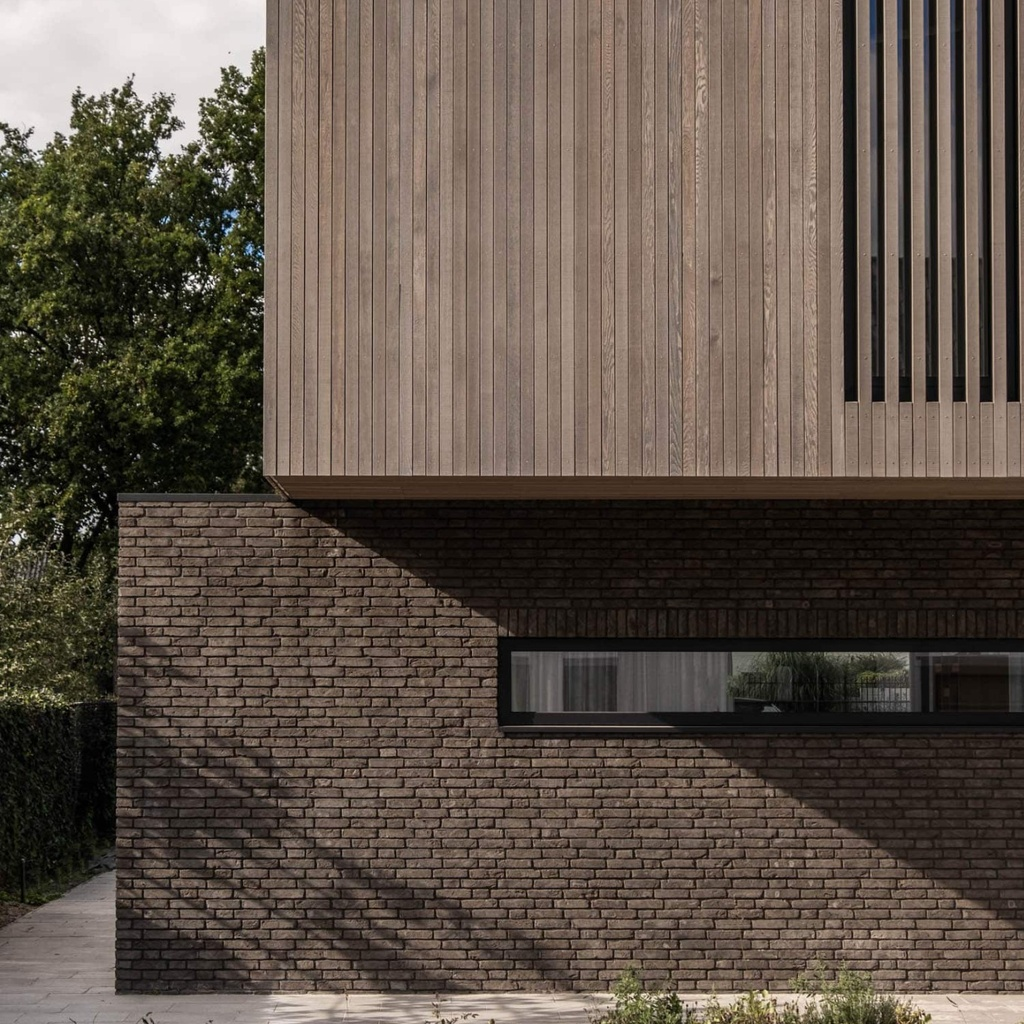
\includegraphics[width=\linewidth]{Images/LoRAs/Geleding/8.jpg} &
      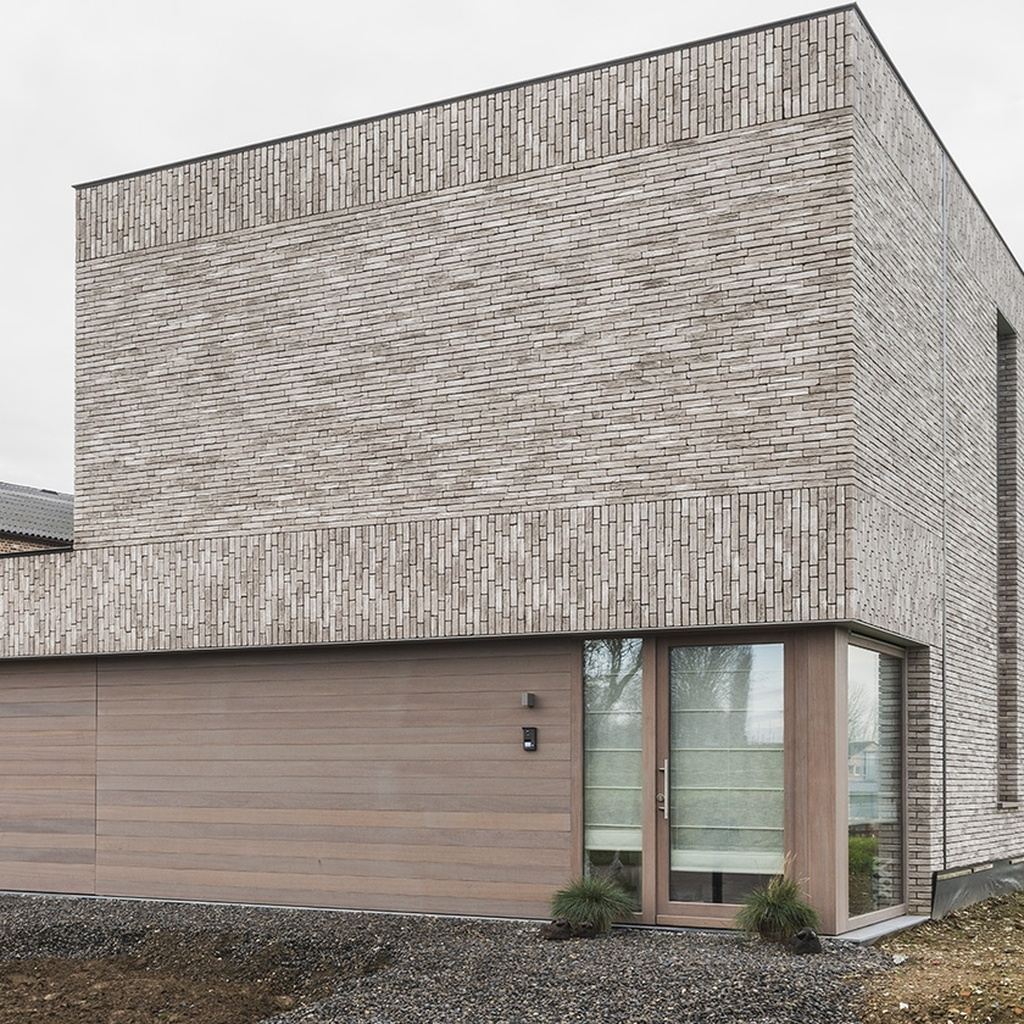
\includegraphics[width=\linewidth]{Images/LoRAs/Geleding/9.jpg} &
      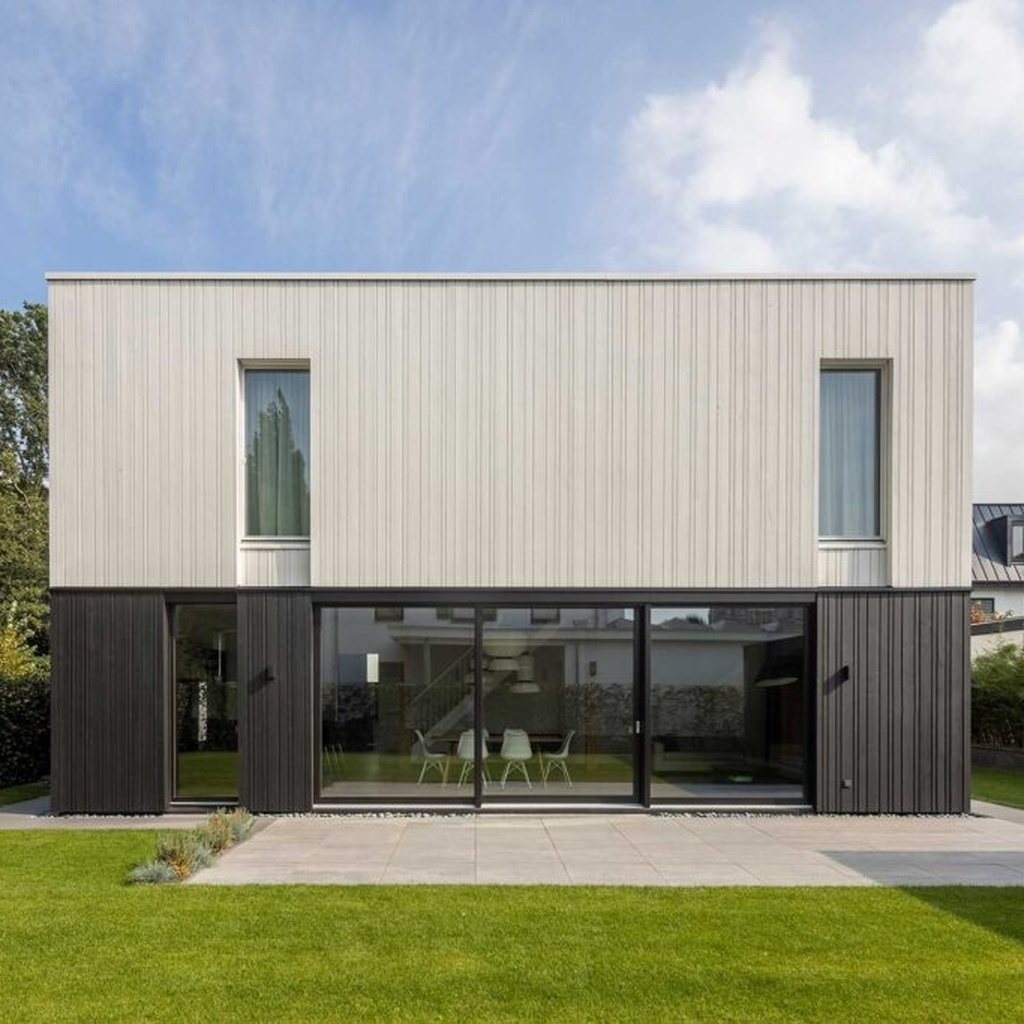
\includegraphics[width=\linewidth]{Images/LoRAs/Geleding/11.jpg} &
      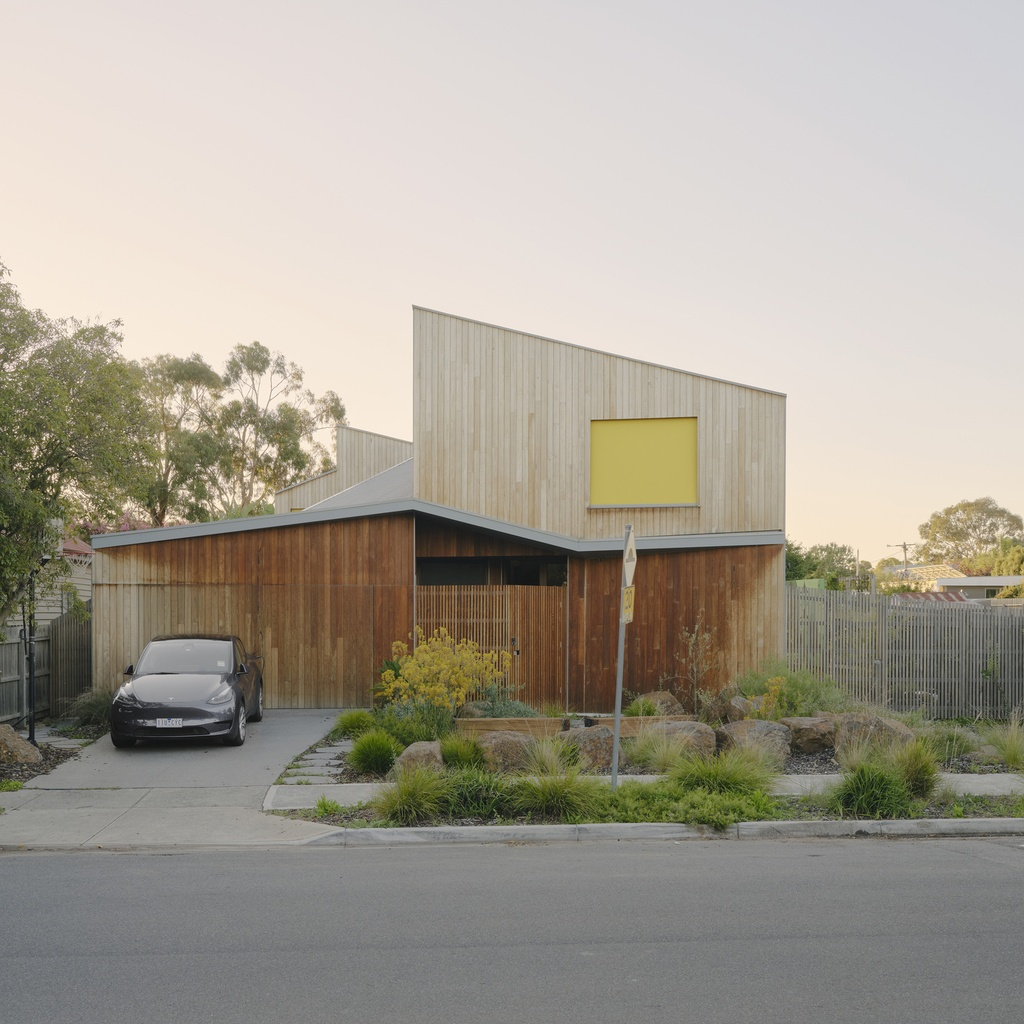
\includegraphics[width=\linewidth]{Images/LoRAs/Geleding/12.jpg} &
      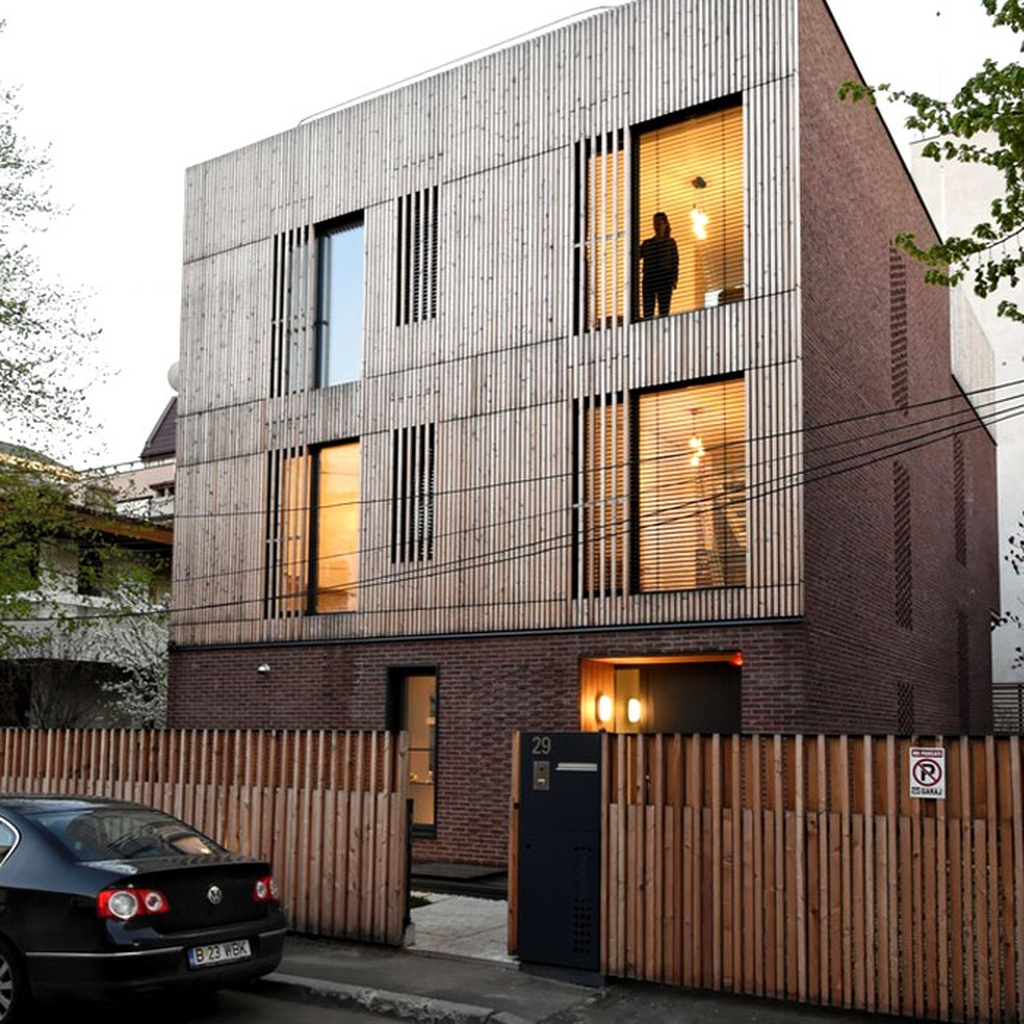
\includegraphics[width=\linewidth]{Images/LoRAs/Geleding/16.jpg} \\[2pt]
    \end{tabular}
    }
  \caption{The images removed from the original geleding dataset.}
  \label{fig:removedgeleding}
\end{figure}
Figure \ref{fig:gridgeleding} portrays the training images for this LoRA.
\begin{figure}[H]
  \centering
  \resizebox{\textwidth}{!}{%
    \begin{tabular}{@{}ccccc@{}}
      % Row 1: images 1–5
      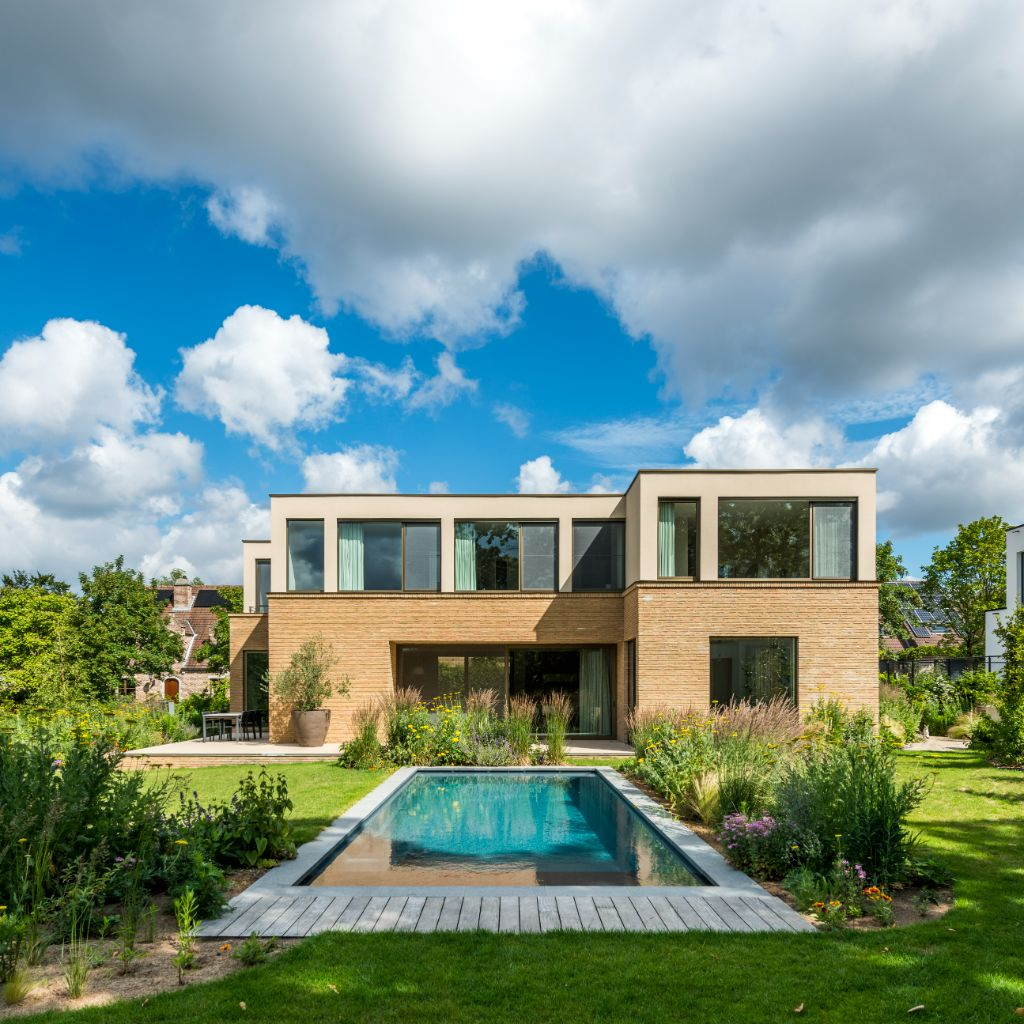
\includegraphics[width=\linewidth]{Images/LoRAs/Geleding/Training_images/1.jpg} &
      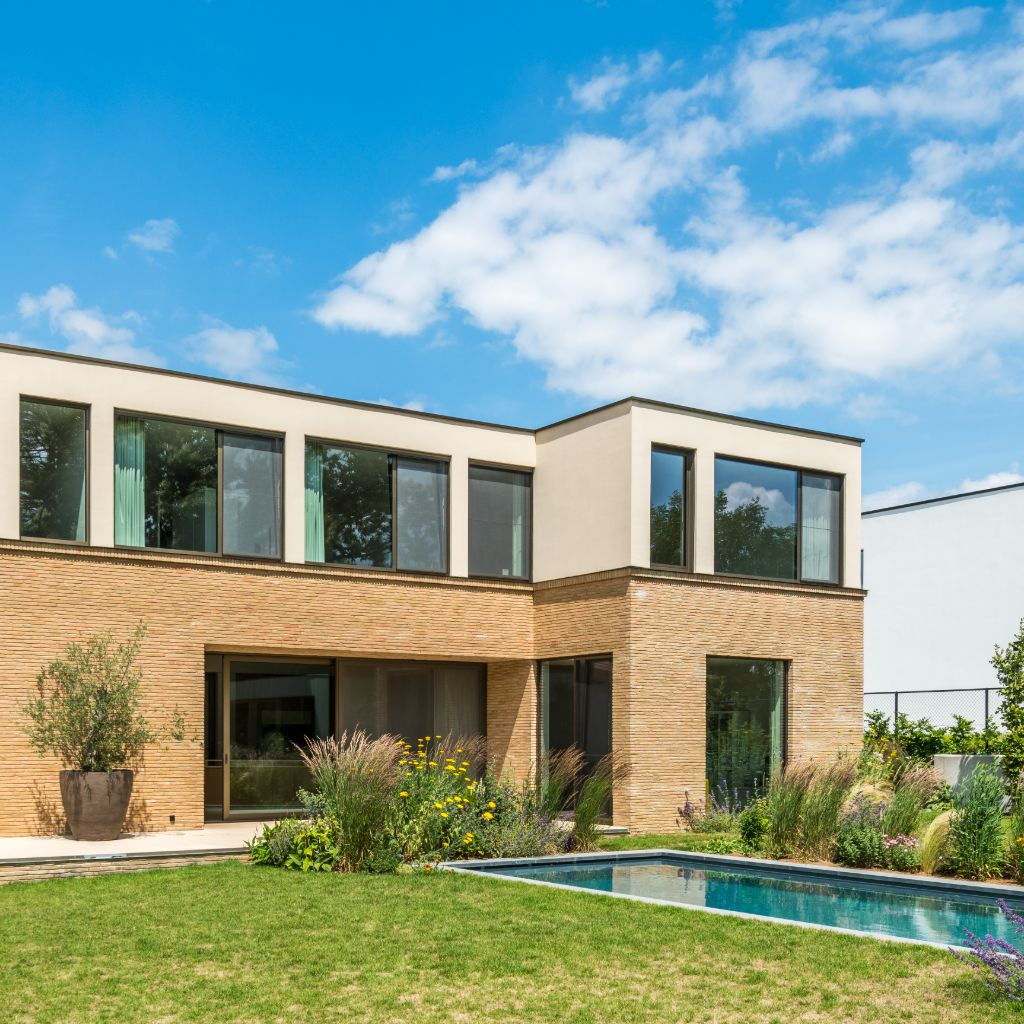
\includegraphics[width=\linewidth]{Images/LoRAs/Geleding/Training_images/2.jpg} &
      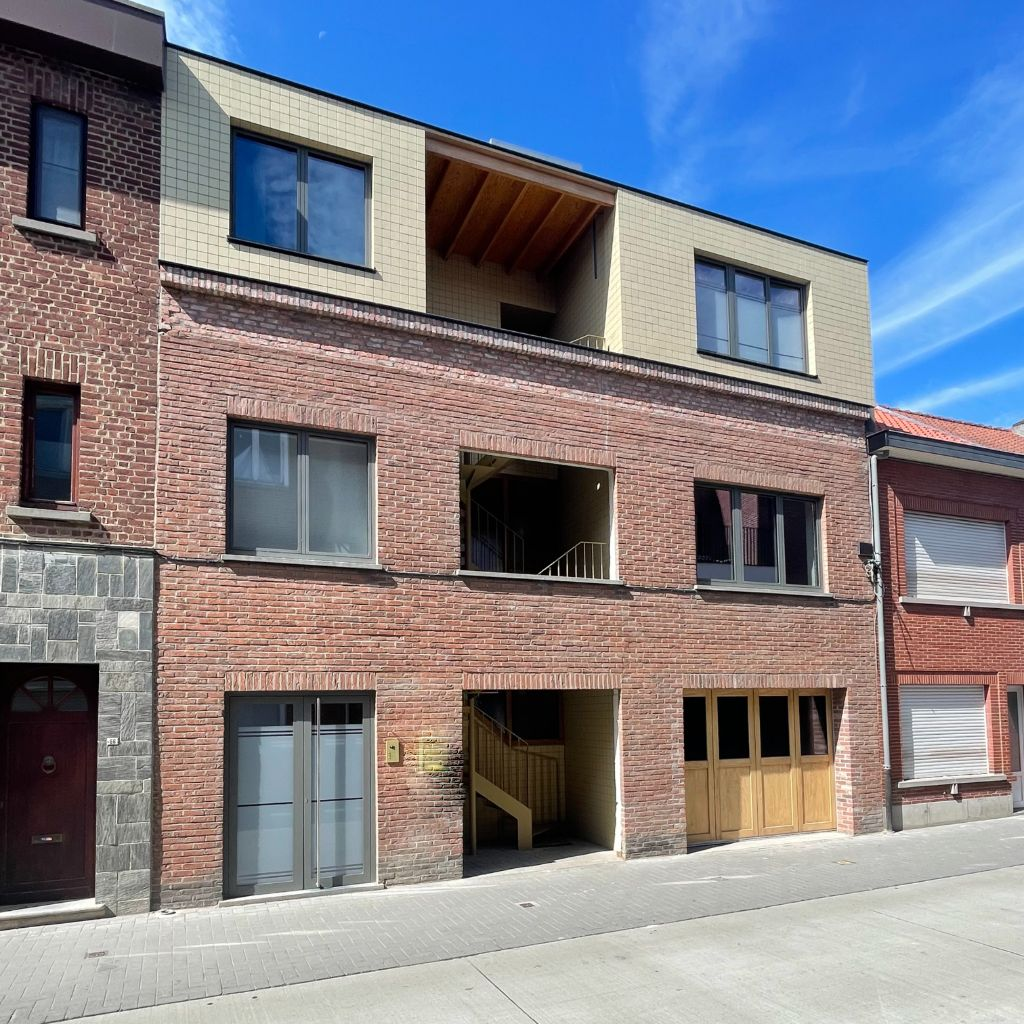
\includegraphics[width=\linewidth]{Images/LoRAs/Geleding/Training_images/3.jpeg} &
      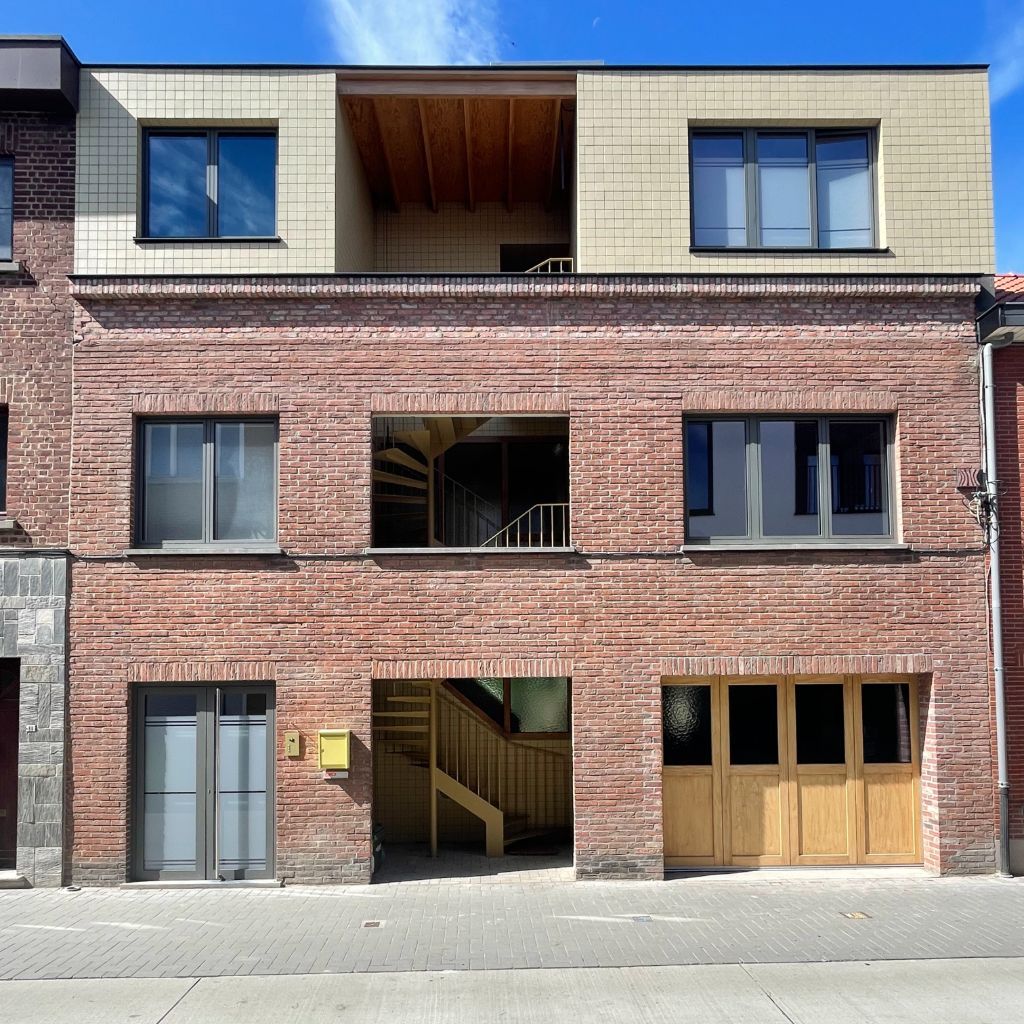
\includegraphics[width=\linewidth]{Images/LoRAs/Geleding/Training_images/4.jpeg} &
      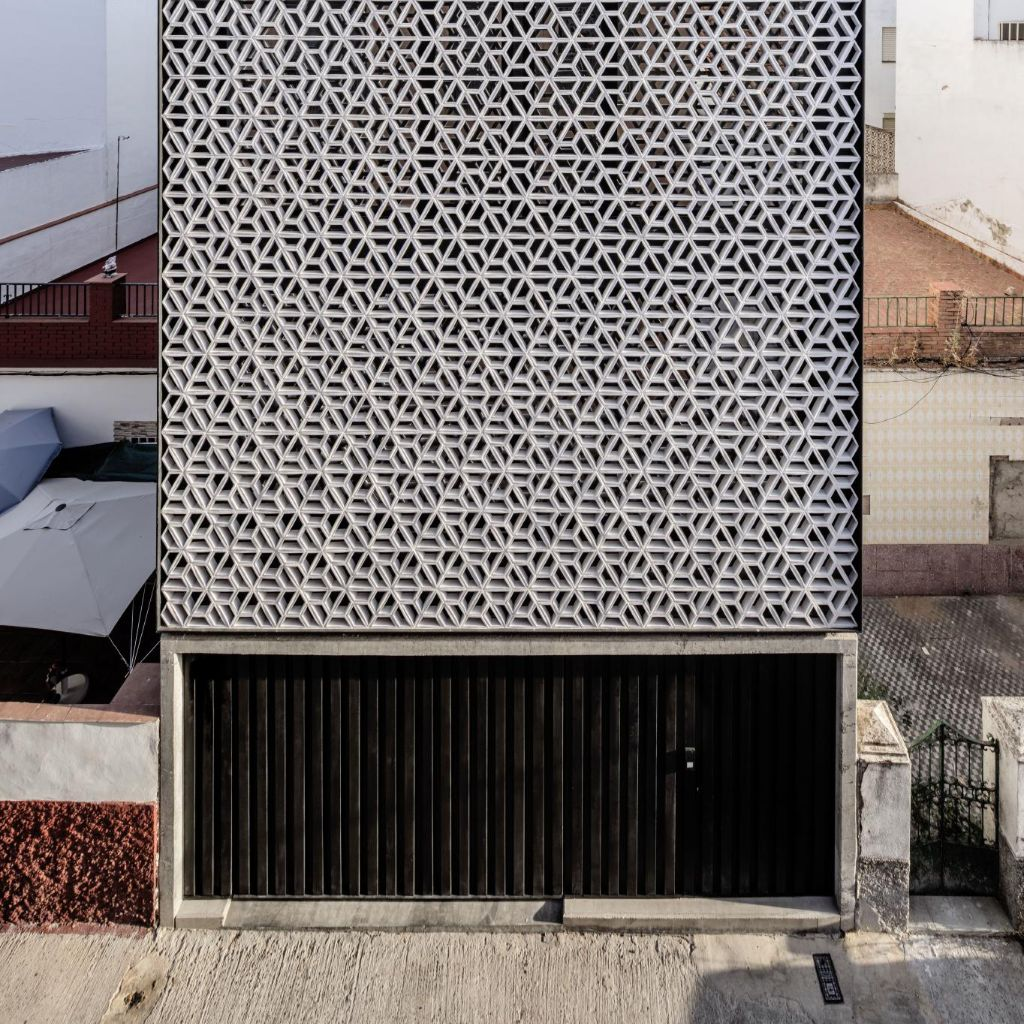
\includegraphics[width=\linewidth]{Images/LoRAs/Geleding/Training_images/5.jpg} \\[2pt]

      % Row 2: images 6–10
      \includegraphics[width=\linewidth]{Images/LoRAs/Geleding/Training_images/6.jpg} &
      \includegraphics[width=\linewidth]{Images/LoRAs/Geleding/Training_images/7.jpg} &
      \includegraphics[width=\linewidth]{Images/LoRAs/Geleding/Training_images/8.jpg} &
      \includegraphics[width=\linewidth]{Images/LoRAs/Geleding/Training_images/9.jpg} &
      \includegraphics[width=\linewidth]{Images/LoRAs/Geleding/Training_images/10.jpg} \\[2pt]

      % Row 3: images 11–15
      \includegraphics[width=\linewidth]{Images/LoRAs/Geleding/Training_images/11.jpg} &
      \includegraphics[width=\linewidth]{Images/LoRAs/Geleding/Training_images/12.jpg} &
      \includegraphics[width=\linewidth]{Images/LoRAs/Geleding/Training_images/13.jpg} &
      \includegraphics[width=\linewidth]{Images/LoRAs/Geleding/Training_images/14.jpg} &
      \includegraphics[width=\linewidth]{Images/LoRAs/Geleding/Training_images/15.jpg} \\
    \end{tabular}%
  }
  \caption{The images used to train the geleding LoRA.}
  \label{fig:gridgeleding}
\end{figure}

\subsection{Finalized datasets for LAVA}
\subsubsection{Modulariteit}
The first LoRA for LAVA is built around modular buildings. This concept was chosen by the architect due to its contemporary relevance and its potential to enable high-quality re-use.\\
Visually, this LoRA emphasizes on generating a grid in the facade.
After validation, four images were left out of the original dataset (figure \ref{fig:removedmodulariteit}): in images 1, 3 and 4, the modularity was insufficiently clear, and in image 2 the wooden building extension felt structurally monolithic, rather than composed of modules.
\begin{figure}[H]
  \centering
   \resizebox{\textwidth}{!}{%
    \begin{tabular}{@{}cccc@{}}
      % Row 1: images 1–2
      \includegraphics[width=\linewidth]{Images/LoRAs/Modulariteit/8.jpg}&
      \includegraphics[width=\linewidth]{Images/LoRAs/Modulariteit/10.jpg}&
      \includegraphics[width=\linewidth]{Images/LoRAs/Modulariteit/12.jpeg}&
      \includegraphics[width=\linewidth]{Images/LoRAs/Modulariteit/14.jpeg}\\
    \end{tabular}
  }
  \caption{The images removed from the original modulariteit dataset.}
  \label{fig:removedmodulariteit}
\end{figure}

Figure \ref{fig:gridmodulariteit} portrays the training images for this LoRA.
\begin{figure}[H]
  \centering
  \resizebox{\textwidth}{!}{%
    \begin{tabular}{@{}ccccc@{}}
      % Row 1: images 1–5
      \includegraphics[width=\linewidth]{Images/LoRAs/Modulariteit/Training_images/1.jpg} &
      \includegraphics[width=\linewidth]{Images/LoRAs/Modulariteit/Training_images/2.jpg} &
      \includegraphics[width=\linewidth]{Images/LoRAs/Modulariteit/Training_images/3.jpeg} &
      \includegraphics[width=\linewidth]{Images/LoRAs/Modulariteit/Training_images/4.jpg} &
      \includegraphics[width=\linewidth]{Images/LoRAs/Modulariteit/Training_images/5.jpg} \\[2pt]

      % Row 2: images 6–10
      \includegraphics[width=\linewidth]{Images/LoRAs/Modulariteit/Training_images/6.jpg} &
      \includegraphics[width=\linewidth]{Images/LoRAs/Modulariteit/Training_images/7.jpg} &
      \includegraphics[width=\linewidth]{Images/LoRAs/Modulariteit/Training_images/8.jpg} &
      \includegraphics[width=\linewidth]{Images/LoRAs/Modulariteit/Training_images/9.png} &
      \includegraphics[width=\linewidth]{Images/LoRAs/Modulariteit/Training_images/10.JPG} \\[2pt]

      % Row 3: images 11–15
      \includegraphics[width=\linewidth]{Images/LoRAs/Modulariteit/Training_images/11.jpg} &
      \includegraphics[width=\linewidth]{Images/LoRAs/Modulariteit/Training_images/12.jpg} &
      \includegraphics[width=\linewidth]{Images/LoRAs/Modulariteit/Training_images/13.jpg} &
      \includegraphics[width=\linewidth]{Images/LoRAs/Modulariteit/Training_images/14.jpg} &
      \includegraphics[width=\linewidth]{Images/LoRAs/Modulariteit/Training_images/15.jpg} \\
    \end{tabular}%
  }
  \caption{The images used to train the Modulariteit LoRA.}
  \label{fig:gridmodulariteit}
\end{figure}
\subsubsection{Ghoek}
The second LoRA portrays rounded facade corners, a formal element often used in LAVA's projects.\\
After validation, two images (Figure \ref{fig:removedghoek}) were excluded from the original dataset. The first contained an excessive number of curved corners, and the second displayed a curve that was too large.
\begin{figure}[H]
  \centering
  % First image
  \includegraphics[width=0.24\textwidth]{Images/LoRAs/Ghoek/2.jpg}%
  \hspace{0.005\textwidth} % small gap; adjust if needed
  % Second image
  \includegraphics[width=0.24\textwidth]{Images/LoRAs/Ghoek/8.jpg}
  \caption{The images removed from the original Ghoek dataset.}
  \label{fig:removedghoek}
\end{figure}
Figure \ref{fig:gridghoek} portrays the training images for this LoRA.
\begin{figure}[H]
  \centering
  \resizebox{\textwidth}{!}{%
    \begin{tabular}{@{}ccccc@{}}
      % Row 1: images 1–5
      \includegraphics[width=\linewidth]{Images/LoRAs/Ghoek/Training_images/1.jpeg} &
      \includegraphics[width=\linewidth]{Images/LoRAs/Ghoek/Training_images/2.jpg} &
      \includegraphics[width=\linewidth]{Images/LoRAs/Ghoek/Training_images/3.jpg} &
      \includegraphics[width=\linewidth]{Images/LoRAs/Ghoek/Training_images/4.jpg} &
      \includegraphics[width=\linewidth]{Images/LoRAs/Ghoek/Training_images/5.jpg} \\[2pt]

      % Row 2: images 6–10
      \includegraphics[width=\linewidth]{Images/LoRAs/Ghoek/Training_images/6.jpeg} &
      \includegraphics[width=\linewidth]{Images/LoRAs/Ghoek/Training_images/7.jpeg} &
      \includegraphics[width=\linewidth]{Images/LoRAs/Ghoek/Training_images/8.jpg} &
      \includegraphics[width=\linewidth]{Images/LoRAs/Ghoek/Training_images/9.jpg} &
      \includegraphics[width=\linewidth]{Images/LoRAs/Ghoek/Training_images/10.JPG} \\[2pt]

      % Row 3: images 11–15
      \includegraphics[width=\linewidth]{Images/LoRAs/Ghoek/Training_images/11.jpg} &
      \includegraphics[width=\linewidth]{Images/LoRAs/Ghoek/Training_images/12.jpg} &
      \includegraphics[width=\linewidth]{Images/LoRAs/Ghoek/Training_images/13.jpg} &
      \makebox[0.19\textwidth]{} &
      \makebox[0.19\textwidth]{} \\
    \end{tabular}%
  }
  \caption{The images used to train the Ghoek LoRA.}
  \label{fig:gridghoek}
\end{figure}

\subsubsection{Plintwerking}
The third and final LoRA for LAVA represents a 'plinth effect', often used in contemporary architecture to differentiate the ground floor of a building from the upper levels.\\
After validation, three images (figure \ref{fig:gridplintwerking}) were removed from the original dataset. In the first and third, the only distinction between the plinth and the upper floors was materiality, which was considered insufficient; in the second, the architect judged that the building was not effectively emphasized in the image, preferring other images of the same building.
\begin{figure}[H]
  \centering
  \includegraphics[width=0.24\textwidth]{Images/LoRAs/Plintwerking/2.jpg}%
  \hspace{0.005\textwidth} 
  \includegraphics[width=0.24\textwidth]{Images/LoRAs/Plintwerking/5.jpeg}
  \hspace{0.005\textwidth}
  \includegraphics[width=0.24\textwidth]{Images/LoRAs/Plintwerking/6.jpg}
  \caption{The images removed from the original Plintwerking dataset.}
  \label{fig:removedplintwerking}
\end{figure}
Figure \ref{fig:gridplintwerking} portrays the training images for this LoRA.
\begin{figure}[H]
  \centering
  \resizebox{\textwidth}{!}{%
    \begin{tabular}{@{}ccccc@{}}
      % Row 1: images 1–5
      \includegraphics[width=\linewidth]{Images/LoRAs/Plintwerking/Training_images/1.jpg} &
      \includegraphics[width=\linewidth]{Images/LoRAs/Plintwerking/Training_images/2.jpg} &
      \includegraphics[width=\linewidth]{Images/LoRAs/Plintwerking/Training_images/3.jpg} &
      \includegraphics[width=\linewidth]{Images/LoRAs/Plintwerking/Training_images/4.jpeg} &
      \includegraphics[width=\linewidth]{Images/LoRAs/Plintwerking/Training_images/5.jpg} \\[2pt]

      % Row 2: images 6–10
      \includegraphics[width=\linewidth]{Images/LoRAs/Plintwerking/Training_images/6.jpg} &
      \includegraphics[width=\linewidth]{Images/LoRAs/Plintwerking/Training_images/7.jpeg} &
      \includegraphics[width=\linewidth]{Images/LoRAs/Plintwerking/Training_images/8.jpeg} &
      \includegraphics[width=\linewidth]{Images/LoRAs/Plintwerking/Training_images/9.jpg} &
      \includegraphics[width=\linewidth]{Images/LoRAs/Plintwerking/Training_images/10.jpg} \\[2pt]

      % Row 3: images 11–12 (plus empty placeholders)
      \includegraphics[width=\linewidth]{Images/LoRAs/Plintwerking/Training_images/11.jpg} &
      \includegraphics[width=\linewidth]{Images/LoRAs/Plintwerking/Training_images/12.jpg} &
      \makebox[0.19\textwidth]{} &
      \makebox[0.19\textwidth]{} &
      \makebox[0.19\textwidth]{} \\
    \end{tabular}%
  }
  \caption{The images used to train the Plintwerking LoRA.}
  \label{fig:gridplintwerking}
\end{figure}
\subsection{Conclusion}
The training datasets for each LoRA were assembled through a workflow of image collection, resizing, and validation by the architects themselves. \\
Initial datasets of 15–19 images per concept were rated by the architects on a 3-point likert scale, which led to the removal of images that poorly illustrated the target feature, whether due to misleading textures, inadequate composition, or stylistic mismatch.

Across the six LoRAs, the finalized image sets contain between 12 and 15 images each. Every retained image clearly exemplifies its respective concept under varied lighting, scale, and perspective conditions. This selection protocol provides high-quality, concept-specific training data.

\newpage
\section{LoRA training methodology}\label{sec:LoRA training methodology}
To train LoRA models on the finalized image datasets, a methodology was developed over the course of several months of experimentation. To train the LoRAs, a cloud service called Replicate (\href{https://replicate.com/}{replicate.com}) was used.\\
Figure \ref{fig:lora-methodology} shows the process of training the LoRA models. This process is iterative; thus, there are multiple versions that each LoRA goes through until it's a finished product.
\begin{figure}[H]
    \centering
    \includegraphics[width=\linewidth]{Images//Methodology/LoRA methodology.jpg}
    \caption{The methodology used to train each of the 6 LoRA models.}
    \label{fig:lora-methodology}
\end{figure}

\subsection{Image captioning}
To guide LoRA training toward learning the target concept, all images were captioned with the custom GPT 'LoRA prompt generator' (section \ref{sec:ChatGPT}). This ensured that the training captions always had the same structure as the prompts used to generate output images.\\
\\
Refining the captions iteratively is essential, because output images of initial versions of the LoRA rarely show satisfactory results. Only after training and evaluating the first versions of the LoRA, one can identify where the LoRA lays its focus the most and modify the captions accordingly. Two frequent problems occuring here are 'overfitting', which happens when the LoRA associates irrelevant details with the concept, and 'underfitting', which happens when the captions are not clear enough and the LoRA does not grasp the concept. Only after some repetitions of captioning, training and testing, the LoRA grasps the concept in the envisioned way.

\subsection{LoRA training}
After a ZIP-file containing all the images and all the captions was created, Ostris' \href{https://replicate.com/ostris/flux-dev-lora-trainer/train}{FLUX.1 [dev] LoRA trainer} on replicate.com was used. This model is based on Ostris' public GitHub-repository 'ai-toolkit' (the repository can be found on \href{https://github.com/ostris/ai-toolkit}{https://github.com/ostris/ai-toolkit}).\\
In the form on the website, the trigger word of the LoRA has to be entered, as well as the amount of steps to train and the lora rank. For all the LoRAs, the steps were kept to the default number of 1000 and the lora rank was kept to 16, concentrating on improving the captions when iterating versions.

\subsection{LoRA testing}
To test the LoRA models, the researcher generated images using the custom ComfyUI workflow and the custom GPT, assessing the LoRA models in several contexts and use cases. After generating numerous images and critically reviewing them, the researcher gets an idea for what the LoRA might improve upon.\\
After testing the LoRA, if the quality is not satisfactory, the researcher went back to the first step of captioning the images and training a new version of the LoRA, after which the cycle repeats.

\subsection{Finalized LoRA}
The LoRA models were finalized when the researcher was satisfied with the generated output images.

\section{Evaluation sessions} \label{sec:Evaluation sessions}
To research how the trained LoRA models could help Flemish architects design, images generated with the LoRA models were evaluated by professional Flemish architects in experimental design phases. 
\subsection{Participants}
For this study, two architectural offices participated, which are both originated in Leuven: DMOA and LAVA. One partner from each office participated in the study. 

\subsection{Structure of the sessions}
\begin{figure}[H]
    \centering
    \includegraphics[width=1\linewidth]{Images/Methodology/timeline_evaluation_sessions.jpg}
    \caption{The chronological structure of the evaluation sessions.}
    \label{fig:timeline}
\end{figure}
Figure \ref{fig:timeline} portrays the structure of the evaluation sessions, which consisted of 2 segments where images were evaluated: a structured segment and an unstructured segment.\\
The \textbf{structured segment} was divided into 3 design phases: sketch design, preliminary design, and presentation (\cite{riba_riba_2024}, part 1 chapter 1). To keep the start of these phases equal for both architects, each phase starts from a new small design brief.\\
After the structured segment, the researcher conducted a brief \textbf{interview} with the participating architects, during which they reflected on the AI-generated images.\\
This was followed by the \textbf{unstructured segment}, in which the LoRA models were applied to images provided by the architects themselves, allowing for an exploration of how the LoRA models perform when integrated into their own design projects.\\~\\
The sketch design and preliminary design phases are focused on \textbf{Text-to-Image generation}, while the presentation phase and unstructured segment are focused on \textbf{Image-to-Image generation} using ControlNet.\\
Each of the phases is explained in more detail in the following sections.
\subsubsection{Sketch design}
For the sketch design phase, the design brief concerned an apartment building  located near a public park in Brussels (figure \ref{fig:sketch-site}), containing public functions (such as stores or workshop spaces) on the ground floor.\\
In this phase, the architects were told to focus on the \textbf{volumetry} of the building.
\begin{figure}[H]
    \centering
    \includegraphics[width=0.75\linewidth]{Images/Methodology/Sketch_design_brief.png}
    \caption{The site for the sketch design phase.}
    \label{fig:sketch-site}
\end{figure}

\subsubsection{Preliminary design}
In the preliminary design phase, the idea is that the volume is already determined; thus, the volumetry for this phase was predetermined by the researcher: a cubic volume. The architects were told to shift their focus to concepts like materiality, composition and execution of the facade.\\
The brief for this phase was to design a freestanding family home for a family of 2 parents and 2 children. \\
\begin{figure}
    \centering
    \includegraphics[width=0.75\linewidth]{Images/Methodology/Preliminary_design_brief.png}
    \caption{The site for the preliminary design phase.}
    \label{fig:preliminary-site}
\end{figure}

\subsection{Presentation}
The presentation phase simulated the stage in architectural design where a presentation has to be held for clients. Since the design would already be finished when starting this phase, images were generated based on the geometry of a 3D-model (figure \ref{fig:presentation-image}) using ControlNet with a Canny preprocessor.
\begin{figure}[H]
    \centering
    \includegraphics[width=0.5\linewidth]{Images//Methodology/presentation_image.png}
    \caption{The image that served as a base for the generated images in the Presentation design phase.}
    \label{fig:presentation-image}
\end{figure}

\subsection{Data collection}
The following data were collected for each participating architect:
\begin{itemize}
    \item Screen and audio recordings of the sessions; 
    \item Video recordings of the sessions.
\end{itemize}

Both sessions were thematically analyzed by the researcher.
\chapter{Results}
This chapter presents the results of two \textbf{evaluation sessions conducted with two professional architects}, hereafter referred to as \textit{architect A} and \textit{architect B}. During these sessions, Each architect evaluated AI-generated images generated using different combinations of the architect's three LoRA models.\\~\\
To facilitate the sessions, the researcher prepared a selection of images in advance, as generating images requires some time; on the Thinkdiffusion server used in the evaluation sessions, one image takes about 30 seconds to generate. Additional images were generated during the sessions themselves, allowing the architect to interact with the image generation process and to observe outputs in real time.\\~\\
The chapter is divided by architect in two sections (Sections \ref{sec: results-A}) and \ref{sec:results-B}) , and within each section by design phase. Finally, section \ref{sec:results-analysis} outlines the most prominent themes of both sessions.
\newpage
\section{Architect A}\label{sec: results-A}
\subsection{Sketch design phase}
\subsubsection{Starting images}
\begin{figure}[H]
  \centering
  {\footnotesize
  \renewcommand{\arraystretch}{1.1}
  \setlength{\tabcolsep}{4pt}
  \begin{tabular}{c c c c c c c c}
    & \shortstack{\textbf{Stamp-}\\\textbf{beton}} 
    & \shortstack{\textbf{3D-}\\\textbf{effect}} 
    & \textbf{Geleding} 
    & \shortstack{\textbf{Stampbeton}\\ \textbf{\& 3D-effect}} 
    & \shortstack{\textbf{Stampbeton}\\ \textbf{\& Geleding}} 
    & \shortstack{\textbf{3D-effect} \&\\ \textbf{Geleding}} 
    & \shortstack{\textbf{Stampbeton,}\\\textbf{3D-effect \&}\\\textbf{Geleding}} \\

    \shortstack{\textbf{With}\\\textbf{LoRA}} & \href{https://github.com/matijspeeters/Thesis/blob/main/Images/Results/Architect-A_Fixed-images/1-sketch_design/Met_lora_00001_.png}{\includegraphics[width=0.12\textwidth]{Images/Results/Architect-A_Fixed-images/1-sketch_design/Met_lora_00001_.png}} & \href{https://github.com/matijspeeters/Thesis/blob/main/Images/Results/Architect-A_Fixed-images/1-sketch_design/Met_lora_00002_.png}{\includegraphics[width=0.12\textwidth]{Images/Results/Architect-A_Fixed-images/1-sketch_design/Met_lora_00002_.png}} &
    \href{https://github.com/matijspeeters/Thesis/blob/main/Images/Results/Architect-A_Fixed-images/1-sketch_design/Met_lora_00017_%20(2).png}{\includegraphics[width=0.12\textwidth]{Images/Results/Architect-A_Fixed-images/1-sketch_design/Met_lora_00017_ (2).png}} &
    \href{https://github.com/matijspeeters/Thesis/blob/main/Images/Results/Architect-A_Fixed-images/1-sketch_design/Met_lora_00029_.png}{\includegraphics[width=0.12\textwidth]{Images/Results/Architect-A_Fixed-images/1-sketch_design/Met_lora_00029_.png}} &
    \href{https://github.com/matijspeeters/Thesis/blob/main/Images/Results/Architect-A_Fixed-images/1-sketch_design/Met_lora_00039_.png}{\includegraphics[width=0.12\textwidth]{Images/Results/Architect-A_Fixed-images/1-sketch_design/Met_lora_00039_.png}} &
    \href{https://github.com/matijspeeters/Thesis/blob/main/Images/Results/Architect-A_Fixed-images/1-sketch_design/Met_lora_00043_%20(1).png}{\includegraphics[width=0.12\textwidth]{Images/Results/Architect-A_Fixed-images/1-sketch_design/Met_lora_00043_ (1).png}} &
    \href{https://github.com/matijspeeters/Thesis/blob/main/Images/Results/Architect-A_Fixed-images/1-sketch_design/Met_lora_00058_.png}{\includegraphics[width=0.12\textwidth]{Images/Results/Architect-A_Fixed-images/1-sketch_design/Met_lora_00058_.png}} \\

    \shortstack{\textbf{Without}\\\textbf{LoRA}} &
    \href{https://github.com/matijspeeters/Thesis/blob/main/Images/Results/Architect-A_Fixed-images/1-sketch_design/Zonder_lora_00001_.png}{\includegraphics[width=0.12\textwidth]{Images/Results/Architect-A_Fixed-images/1-sketch_design/Zonder_lora_00001_.png}} &
    \href{https://github.com/matijspeeters/Thesis/blob/main/Images/Results/Architect-A_Fixed-images/1-sketch_design/Zonder_lora_00002_.png}{\includegraphics[width=0.12\textwidth]{Images/Results/Architect-A_Fixed-images/1-sketch_design/Zonder_lora_00002_.png}} &
    \href{https://github.com/matijspeeters/Thesis/blob/main/Images/Results/Architect-A_Fixed-images/1-sketch_design/Zonder_lora_00017_%20(1).png}{\includegraphics[width=0.12\textwidth]{Images/Results/Architect-A_Fixed-images/1-sketch_design/Zonder_lora_00017_ (1).png}} &
    \href{https://github.com/matijspeeters/Thesis/blob/main/Images/Results/Architect-A_Fixed-images/1-sketch_design/Zonder_lora_00029_.png}{\includegraphics[width=0.12\textwidth]{Images/Results/Architect-A_Fixed-images/1-sketch_design/Zonder_lora_00029_.png}} &
    \href{https://github.com/matijspeeters/Thesis/blob/main/Images/Results/Architect-A_Fixed-images/1-sketch_design/Zonder_lora_00039_.png}{\includegraphics[width=0.12\textwidth]{Images/Results/Architect-A_Fixed-images/1-sketch_design/Zonder_lora_00039_.png}} &
    \href{https://github.com/matijspeeters/Thesis/blob/main/Images/Results/Architect-A_Fixed-images/1-sketch_design/Zonder_lora_00043_%20(1).png}{\includegraphics[width=0.12\textwidth]{Images/Results/Architect-A_Fixed-images/1-sketch_design/Zonder_lora_00043_ (1).png}} &
    \href{https://github.com/matijspeeters/Thesis/blob/main/Images/Results/Architect-A_Fixed-images/1-sketch_design/Zonder_lora_00058_.png}{\includegraphics[width=0.12\textwidth]{Images/Results/Architect-A_Fixed-images/1-sketch_design/Zonder_lora_00058_.png}} \\
  \end{tabular}
  }
  \caption{Starting images in the sketch design phase of architect A.}
  \label{fig:horizontal-lora-comparison}
\end{figure}
\subsubsection{Selected starting image}
Architect A selected the image in figure \ref{fig:A-sketch-selected}, which was generated with the \textbf{3D-effect} and \textbf{Geleding} models. His reasons were two-fold: the 'warm facade cladding' and 'a clear connection to the ground level'.
\begin{figure}[H]
    \centering
    \href{https://github.com/matijspeeters/Thesis/blob/main/Images/Results/Architect-A_Fixed-images/1-sketch_design/Met_lora_00043_%20(1).png}{\includegraphics[width=0.3\linewidth]{Images/Results/Architect-A_Fixed-images/1-sketch_design/Met_lora_00043_ (1).png}}
    \caption{Architect A's selected starting image for the sketch design phase.}
    \label{fig:A-sketch-selected}
\end{figure}
\subsubsection{Preferred generated images}
Architect A selected 3 preferred images (figure \ref{fig:A-sketch-favourite}) among the generated images during the sketch design phase. In his opinion, image 1 and 2 shared a 'combination of old and new'. The building in image 3 was 'playing with volumes, rather than referring to something'. It 'introduces a very strong gesture' and 'interacts with nature'.
\begin{figure}[H]
    \centering
    \begin{tabular}{ccc}
         \href{https://github.com/matijspeeters/Thesis/blob/main/Images/Results/Architect%20A/1.%20sketch%20phase/Met_lora_00126_.png}{\includegraphics[width=0.3\linewidth]{Images/Results/Architect A/1. sketch phase/Met_lora_00126_.png}}
         & \href{https://github.com/matijspeeters/Thesis/blob/main/Images/Results/Architect%20A/1.%20sketch%20phase/Met_lora_00139_.png}{\includegraphics[width=0.3\linewidth]{Images/Results/Architect A/1. sketch phase/Met_lora_00139_.png}}
         & \href{https://github.com/matijspeeters/Thesis/blob/main/Images/Results/Architect%20A/1.%20sketch%20phase/Zonder_lora_00144_.png}{\includegraphics[width=0.3\linewidth]{Images/Results/Architect A/1. sketch phase/Zonder_lora_00144_.png}}\\
         \textit{(1)} & \textit{(2)} & \textit{(3)}
    \end{tabular}
    \caption{Architect A's favourite images in the sketch design phase.}
    \label{fig:A-sketch-favourite}
\end{figure}
\subsection{Preliminary design phase}
\subsubsection{Starting images}
\begin{figure}[H]
  \centering
  {\footnotesize
  \renewcommand{\arraystretch}{1.1}
  \setlength{\tabcolsep}{4pt}
  \begin{tabular}{c c c c c c c c}
    & \shortstack{\textbf{Stamp-}\\\textbf{beton}} 
    & \shortstack{\textbf{3D-}\\\textbf{effect}} 
    & \textbf{Geleding} 
    & \shortstack{\textbf{Stampbeton}\\ \textbf{\& 3D-effect}} 
    & \shortstack{\textbf{Stampbeton}\\ \textbf{\& Geleding}} 
    & \shortstack{\textbf{3D-effect} \&\\ \textbf{Geleding}} 
    & \shortstack{\textbf{Stampbeton,}\\\textbf{3D-effect \&}\\\textbf{Geleding}} \\

    \shortstack{\textbf{With}\\\textbf{LoRA}} & 
    \href{https://github.com/matijspeeters/Thesis/blob/main/Images/Results/Architect-A_Fixed-images/2-preliminary_design/Met_lora_00059_%20(1).png}{\includegraphics[width=0.12\textwidth]{Images/Results/Architect-A_Fixed-images/2-preliminary_design/Met_lora_00059_ (1).png}} & 
    \href{https://github.com/matijspeeters/Thesis/blob/main/Images/Results/Architect-A_Fixed-images/2-preliminary_design/Met_lora_00061_.png}{\includegraphics[width=0.12\textwidth]{Images/Results/Architect-A_Fixed-images/2-preliminary_design/Met_lora_00061_.png}} &
    \href{https://github.com/matijspeeters/Thesis/blob/main/Images/Results/Architect-A_Fixed-images/2-preliminary_design/Met_lora_00069_%20(1).png}{\includegraphics[width=0.12\textwidth]{Images/Results/Architect-A_Fixed-images/2-preliminary_design/Met_lora_00069_ (1).png}} &
    \href{https://github.com/matijspeeters/Thesis/blob/main/Images/Results/Architect-A_Fixed-images/2-preliminary_design/Met_lora_00080_.png}{\includegraphics[width=0.12\textwidth]{Images/Results/Architect-A_Fixed-images/2-preliminary_design/Met_lora_00080_.png}} &
    \href{https://github.com/matijspeeters/Thesis/blob/main/Images/Results/Architect-A_Fixed-images/2-preliminary_design/Met_lora_00089_.png}{\includegraphics[width=0.12\textwidth]{Images/Results/Architect-A_Fixed-images/2-preliminary_design/Met_lora_00089_.png}} &
    \href{https://github.com/matijspeeters/Thesis/blob/main/Images/Results/Architect-A_Fixed-images/2-preliminary_design/Met_lora_00091_.png}{\includegraphics[width=0.12\textwidth]{Images/Results/Architect-A_Fixed-images/2-preliminary_design/Met_lora_00091_.png}} &
    \href{https://github.com/matijspeeters/Thesis/blob/main/Images/Results/Architect-A_Fixed-images/2-preliminary_design/Met_lora_00095_.png}{\includegraphics[width=0.12\textwidth]{Images/Results/Architect-A_Fixed-images/2-preliminary_design/Met_lora_00095_.png}} \\

    \shortstack{\textbf{Without}\\\textbf{LoRA}} &
    \href{https://github.com/matijspeeters/Thesis/blob/main/Images/Results/Architect-A_Fixed-images/2-preliminary_design/Zonder_lora_00059_%20(1).png}{\includegraphics[width=0.12\textwidth]{Images/Results/Architect-A_Fixed-images/2-preliminary_design/Zonder_lora_00059_ (1).png}} &
    \href{https://github.com/matijspeeters/Thesis/blob/main/Images/Results/Architect-A_Fixed-images/2-preliminary_design/Zonder_lora_00061_.png}{\includegraphics[width=0.12\textwidth]{Images/Results/Architect-A_Fixed-images/2-preliminary_design/Zonder_lora_00061_.png}} &
    \href{https://github.com/matijspeeters/Thesis/blob/main/Images/Results/Architect-A_Fixed-images/2-preliminary_design/Zonder_lora_00069_%20(1).png}{\includegraphics[width=0.12\textwidth]{Images/Results/Architect-A_Fixed-images/2-preliminary_design/Zonder_lora_00069_ (1).png}} &
    \href{https://github.com/matijspeeters/Thesis/blob/main/Images/Results/Architect-A_Fixed-images/2-preliminary_design/Zonder_lora_00080_.png}{\includegraphics[width=0.12\textwidth]{Images/Results/Architect-A_Fixed-images/2-preliminary_design/Zonder_lora_00080_.png}} &
    \href{https://github.com/matijspeeters/Thesis/blob/main/Images/Results/Architect-A_Fixed-images/2-preliminary_design/Zonder_lora_00089_.png}{\includegraphics[width=0.12\textwidth]{Images/Results/Architect-A_Fixed-images/2-preliminary_design/Zonder_lora_00089_.png}} &
    \href{https://github.com/matijspeeters/Thesis/blob/main/Images/Results/Architect-A_Fixed-images/2-preliminary_design/Zonder_lora_00091_.png}{\includegraphics[width=0.12\textwidth]{Images/Results/Architect-A_Fixed-images/2-preliminary_design/Zonder_lora_00091_.png}} &
    \href{https://github.com/matijspeeters/Thesis/blob/main/Images/Results/Architect-A_Fixed-images/2-preliminary_design/Zonder_lora_00095_.png}{\includegraphics[width=0.12\textwidth]{Images/Results/Architect-A_Fixed-images/2-preliminary_design/Zonder_lora_00095_.png}} \\
  \end{tabular}
  }
  \caption{Starting images in the preliminary design phase of architect A.}
  \label{fig:horizontal-lora-comparison}
\end{figure}
\subsubsection{Selected starting image}
Architect A selected the image in figure \ref{fig:A-preliminary-selected}, which was generated with the \textbf{stampbeton} and \textbf{3D-effect} models. 
\begin{figure}[H]
    \centering
    \href{https://github.com/matijspeeters/Thesis/blob/main/Images/Results/Architect-A_Fixed-images/2-preliminary_design/Met_lora_00080_.png}{\includegraphics[width=0.3\linewidth]{Images/Results/Architect-A_Fixed-images/2-preliminary_design/Met_lora_00080_.png}}
    \caption{Architect A's selected starting image for the preliminary design phase.}
    \label{fig:A-preliminary-selected}
\end{figure}
\subsubsection{Preferred generated images}
Architect A chose two preferred images among the images generated during this design phase. 
\begin{itemize}
    \item Image 1 was created with LoRAs. Architect A chose this image because
    \item Image 2 was created without LoRAs. Architect A chose this image because 
\end{itemize}
\begin{figure}[H]
    \centering
    \begin{tabular}{cc}
         \href{https://github.com/matijspeeters/Thesis/blob/main/Images/Results/Architect%20A/2.%20Preliminary%20phase/Met_lora_00004_.png}{\includegraphics[width=0.3\linewidth]{Images/Results/Architect A/2. Preliminary phase/Met_lora_00004_.png}} & \href{https://github.com/matijspeeters/Thesis/blob/main/Images/Results/Architect%20A/2.%20Preliminary%20phase/Zonder_lora_00146_.png}{\includegraphics[width=0.3\linewidth]{Images/Results/Architect A/2. Preliminary phase/Zonder_lora_00146_.png}}\\
         \textit{(1)} & \textit{(2)}
    \end{tabular}
    \caption{Architect A's favourite images in the preliminary design phase.}
    \label{fig:A-preliminary-preferred}
\end{figure}

\subsection{Presentation phase}
\subsubsection{Starting images}
\begin{figure}[H]
  \centering
  {\footnotesize
  \renewcommand{\arraystretch}{1.1}
  \setlength{\tabcolsep}{4pt}
  \begin{tabular}{c c c c c c c c}
    & \shortstack{\textbf{Stamp-}\\\textbf{beton}} 
    & \shortstack{\textbf{3D-}\\\textbf{effect}} 
    & \textbf{Geleding} 
    & \shortstack{\textbf{Stampbeton}\\ \textbf{\& 3D-effect}} 
    & \shortstack{\textbf{Stampbeton}\\ \textbf{\& Geleding}} 
    & \shortstack{\textbf{3D-effect} \&\\ \textbf{Geleding}} 
    & \shortstack{\textbf{Stampbeton,}\\\textbf{3D-effect \&}\\\textbf{Geleding}} \\

    \shortstack{\textbf{With}\\\textbf{LoRA}} & 
    \href{https://github.com/matijspeeters/Thesis/blob/main/Images/Results/Architect-A_Fixed-images/3-presentation/Met_lora_00097_.png}{\includegraphics[width=0.12\textwidth]{Images/Results/Architect-A_Fixed-images/3-presentation/Met_lora_00097_.png}} & 
    \href{https://github.com/matijspeeters/Thesis/blob/main/Images/Results/Architect-A_Fixed-images/3-presentation/Met_lora_00100_.png}{\includegraphics[width=0.12\textwidth]{Images/Results/Architect-A_Fixed-images/3-presentation/Met_lora_00100_.png}} &
    \href{https://github.com/matijspeeters/Thesis/blob/main/Images/Results/Architect-A_Fixed-images/3-presentation/Met_lora_00106_.png}{\includegraphics[width=0.12\textwidth]{Images/Results/Architect-A_Fixed-images/3-presentation/Met_lora_00106_.png}} &
    \href{https://github.com/matijspeeters/Thesis/blob/main/Images/Results/Architect-A_Fixed-images/3-presentation/Met_lora_00111_.png}{\includegraphics[width=0.12\textwidth]{Images/Results/Architect-A_Fixed-images/3-presentation/Met_lora_00111_.png}} &
    \href{https://github.com/matijspeeters/Thesis/blob/main/Images/Results/Architect-A_Fixed-images/3-presentation/Met_lora_00115_.png}{\includegraphics[width=0.12\textwidth]{Images/Results/Architect-A_Fixed-images/3-presentation/Met_lora_00115_.png}} &
    \href{https://github.com/matijspeeters/Thesis/blob/main/Images/Results/Architect-A_Fixed-images/3-presentation/Met_lora_00117_.png}{\includegraphics[width=0.12\textwidth]{Images/Results/Architect-A_Fixed-images/3-presentation/Met_lora_00117_.png}} &
    \href{https://github.com/matijspeeters/Thesis/blob/main/Images/Results/Architect-A_Fixed-images/3-presentation/Met_lora_00121_.png}{\includegraphics[width=0.12\textwidth]{Images/Results/Architect-A_Fixed-images/3-presentation/Met_lora_00121_.png}} \\

    \shortstack{\textbf{Without}\\\textbf{LoRA}} &
    \href{https://github.com/matijspeeters/Thesis/blob/main/Images/Results/Architect-A_Fixed-images/3-presentation/Zonder_lora_00097_.png}{\includegraphics[width=0.12\textwidth]{Images/Results/Architect-A_Fixed-images/3-presentation/Zonder_lora_00097_.png}} &
    \href{https://github.com/matijspeeters/Thesis/blob/main/Images/Results/Architect-A_Fixed-images/3-presentation/Zonder_lora_00100_.png}{\includegraphics[width=0.12\textwidth]{Images/Results/Architect-A_Fixed-images/3-presentation/Zonder_lora_00100_.png}} &
    \href{https://github.com/matijspeeters/Thesis/blob/main/Images/Results/Architect-A_Fixed-images/3-presentation/Zonder_lora_00106_.png}{\includegraphics[width=0.12\textwidth]{Images/Results/Architect-A_Fixed-images/3-presentation/Zonder_lora_00106_.png}} &
    \href{https://github.com/matijspeeters/Thesis/blob/main/Images/Results/Architect-A_Fixed-images/3-presentation/Zonder_lora_00111_.png}{\includegraphics[width=0.12\textwidth]{Images/Results/Architect-A_Fixed-images/3-presentation/Zonder_lora_00111_.png}} &
    \href{https://github.com/matijspeeters/Thesis/blob/main/Images/Results/Architect-A_Fixed-images/3-presentation/Zonder_lora_00115_.png}{\includegraphics[width=0.12\textwidth]{Images/Results/Architect-A_Fixed-images/3-presentation/Zonder_lora_00115_.png}} &
    \href{https://github.com/matijspeeters/Thesis/blob/main/Images/Results/Architect-A_Fixed-images/3-presentation/Zonder_lora_00117_.png}{\includegraphics[width=0.12\textwidth]{Images/Results/Architect-A_Fixed-images/3-presentation/Zonder_lora_00117_.png}} &
    \href{https://github.com/matijspeeters/Thesis/blob/main/Images/Results/Architect-A_Fixed-images/3-presentation/Zonder_lora_00121_.png}{\includegraphics[width=0.12\textwidth]{Images/Results/Architect-A_Fixed-images/3-presentation/Zonder_lora_00121_.png}} \\
  \end{tabular}
  }
  \caption{Starting images in the presentation phase of architect A.}
  \label{fig:horizontal-lora-comparison}
\end{figure}

\subsubsection{Selected starting image}
Architect A selected the image in figure \ref{fig:A-presentation-selected} , which was generated with the stampbeton LoRA. His reasons were the beautiful stamped concrete, and the interaction of the building with the environment. He could 'imagine an interesting location plan'. Additionally, the unusual shape of the roof 'suggests something below it' and 'allows for fun spaces inside'.
\begin{figure}[H]
    \centering
    \href{https://github.com/matijspeeters/Thesis/blob/main/Images/Results/Architect-A_Fixed-images/3-presentation/Met_lora_00097_.png}{\includegraphics[width=0.3\linewidth]{Images/Results/Architect-A_Fixed-images/3-presentation/Met_lora_00097_.png}}
    \caption{Architect A's selected starting image for the presentation phase.}
    \label{fig:A-presentation-selected}
\end{figure}

\subsubsection{Preferred generated images}
Architect A chose two preferred images among the images generated during this design phase. Both images were created with the \textbf{stampbeton} LoRA. The reasons for image \ref{fig:A-presentation-preferred-A} were the 'layering in the bottom zone, the very simple and balanced volumetry, and the beautiful detailing in the roof'. The reasons for image \ref{fig:A-presentation-preferred-B} were the 'simple volumetry and good stamped concrete'.
\begin{figure}[H]
    \centering
    \begin{subfigure}[b]{0.3\textwidth}
        \centering
        \href{https://github.com/matijspeeters/Thesis/blob/main/Images/Results/Architect%20A/3.%20Presentation%20phase/Met_lora_00002_.png}{\includegraphics[width=\textwidth]{Images/Results/Architect A/3. Presentation phase/Met_lora_00002_.png}}
        \caption{}
        \label{fig:A-presentation-preferred-A}
    \end{subfigure}
    \begin{subfigure}[b]{0.3\textwidth}
        \centering
         \href{https://github.com/matijspeeters/Thesis/blob/main/Images/Results/Architect%20A/3.%20Presentation%20phase/Met_lora_00006_.png}{\includegraphics[width=\textwidth]{Images/Results/Architect A/3. Presentation phase/Met_lora_00006_.png}}
         \caption{}
         \label{fig:A-presentation-preferred-B}
    \end{subfigure}
    \caption{Architect A's preferred images in the presentation phase.}
    \label{fig:A-presentation-preferred}
\end{figure}
\newpage
\subsection{Unstructured phase}
During the unstructured phase, architect A provided several sketches of projects that their office is working on. This section portrays a representative selection of AI-generated images based on these sketches, providing an oversight of how this tool worked based on the architects' sketches.\\
All images were generated by uploading the sketch to the custom GPT, and asking it to write a prompt for that building. Then, this prompt was used in combination with ControlNet, to generate images based on this sketch. Two preprocessors were used for this: canny edge detection and a depth map.\\
For each sketch, only a representative selection of generated images (with and without LoRA) is shown here. All generated images can be found in the appendix of this thesis (chapter \ref{appendix}).
\subsubsection{Sketch 1}
\begin{figure}[H]
    \centering
    \begin{subfigure}[b]{0.3\textwidth}
        \centering
        \includegraphics[width=\textwidth]{Images/Results/Architect-A_unstructured-phase/sketches/sketch_1.png}
        \caption{}
        \label{A-unstructured-1-sketch}
    \end{subfigure}
    \begin{subfigure}[b]{0.3\textwidth}
        \centering 
        \includegraphics[width=\textwidth]{Images/Results/Architect-A_unstructured-phase/sketches/sketch_1_preprocessed.png}
        \caption{}
        \label{A-unstructured-1-sketch-prep}
    \end{subfigure}
    \caption{The first original image provided by architect A (a) and the canny-preprocessed image (b).}
    \label{fig:placeholder}
\end{figure}
To generate images based on this sketch, the architect chose to include all 3 LoRAs: the ground floor of the building should be made out of stampbeton, there is a 3D-effect because of the balconies, and there is an articulation because of the difference between ground floor and the floors above. The researcher wrote a prompt with the custom GPT based on the image, and used the canny edge preprocessor to start generating images with ControlNet.
\begin{figure}[H]
  \centering
  {\footnotesize
  \renewcommand{\arraystretch}{1.1}
  \setlength{\tabcolsep}{4pt}
  \begin{tabular}{c c c c}
    \textbf{With LoRA} &
    \includegraphics[width=0.25\textwidth]{Images/Results/Architect-A_unstructured-phase/generated_images/1/Met_lora_00001_.png} &
    \includegraphics[width=0.25\textwidth]{Images/Results/Architect-A_unstructured-phase/generated_images/1/Met_lora_00002_.png} &
    \includegraphics[width=0.25\textwidth]{Images/Results/Architect-A_unstructured-phase/generated_images/1/Met_lora_00005_.png} \\

    \textbf{Without LoRA} &
    \includegraphics[width=0.25\textwidth]{Images/Results/Architect-A_unstructured-phase/generated_images/1/Zonder_lora_00001_.png} &
    \includegraphics[width=0.25\textwidth]{Images/Results/Architect-A_unstructured-phase/generated_images/1/Zonder_lora_00002_.png} &
    \includegraphics[width=0.25\textwidth]{Images/Results/Architect-A_unstructured-phase/generated_images/1/Zonder_lora_00005_.png} \\
  \end{tabular}
  }
  \caption{Comparison of results with and without LoRA, generated from architect A's first sketch.}
  \label{fig:lora-comparison}
\end{figure}
\subsubsection{Sketch 2}
\begin{figure}[H]
    \centering
    \begin{subfigure}[b]{0.3\textwidth}
        \centering
        \includegraphics[width=\textwidth]{Images/Results/Architect-A_unstructured-phase/sketches/sketch_2.png}
        \caption{}
        \label{A-unstructured-1-sketch}
    \end{subfigure}
    \begin{subfigure}[b]{0.3\textwidth}
        \centering 
        \includegraphics[width=\textwidth]{Images/Results/Architect-A_unstructured-phase/sketches/sketch_2_preprocessed.png}
        \caption{}
        \label{A-unstructured-1-sketch-prep}
    \end{subfigure}
    \caption{The second original image provided by architect A (a) and the canny-preprocessed image (b).}
    \label{fig:placeholder}
\end{figure}
For this sketch, the architect provided a view of the rear facade of the same building. He chose to only use the 3D-effect LoRA, for the terraces and balconies.\\
Creating the first images, the GPT interpreted the lines on the adjacent houses as a canal, including it in the prompt. The diffusion model, then, overinterpreted this, generating the building next to a canal, as can be seen in figure \ref{fig:lora-comparison-2wide}. After this, the prompt was changed and these images were generated 
\newcolumntype{M}[1]{>{\centering\arraybackslash}m{#1}}
\begin{figure}[H]
  \centering
  {\footnotesize
  \renewcommand{\arraystretch}{1.1}
  \setlength{\tabcolsep}{4pt}
  \begin{tabular}{c c c c}
    \textbf{With LoRA} &
    \includegraphics[width=0.25\textwidth]{Images/Results/Architect-A_unstructured-phase/generated_images/2/Met_lora_00008_.png} &
    \includegraphics[width=0.25\textwidth]{Images/Results/Architect-A_unstructured-phase/generated_images/2/Met_lora_00012_.png} &
    \includegraphics[width=0.25\textwidth]{Images/Results/Architect-A_unstructured-phase/generated_images/2/Met_lora_00013_.png} \\

    \textbf{Without LoRA} &
    \includegraphics[width=0.25\textwidth]{Images/Results/Architect-A_unstructured-phase/generated_images/2/Zonder_lora_00008_.png} &
    \includegraphics[width=0.25\textwidth]{Images/Results/Architect-A_unstructured-phase/generated_images/2/Zonder_lora_00012_.png} & \includegraphics[width=0.25\textwidth]{Images/Results/Architect-A_unstructured-phase/generated_images/2/Zonder_lora_00013_.png} \\
  \end{tabular}
  }
  \caption{Comparison of results with and without LoRA, generated from architect A's second sketch.}
  \label{fig:lora-comparison-2wide}
\end{figure}
After this, the researcher attempted to generate images with a depth map preprocessor (figure \ref{fig:depth map}).
\begin{figure}[H]
    \centering
    \includegraphics[width=0.3\linewidth]{Images/Results/Architect-A_unstructured-phase/sketches/sketch_2_preprocessed_2.png}
    \caption{The depth map based on architect A's second sketch.}
    \label{fig:depth map}
\end{figure}

\section{Architect B} \label{sec:results-B}
\subsection{Sketch design phase}
\subsubsection{Starting images}
\begin{figure}[H]
  \centering
  {\footnotesize
  \renewcommand{\arraystretch}{1.1}
  \setlength{\tabcolsep}{4pt}
  \begin{tabular}{c c c c c c c c}
    & \textbf{Ghoek} & \textbf{Modulariteit} & \shortstack{\textbf{Plint-}\\\textbf{werking}}
    & \shortstack{\textbf{Ghoek \&}\\ \textbf{modulari-}\\\textbf{teit}} 
    & \shortstack{\textbf{Ghoek \&}\\ \textbf{Plintwerking}} 
    & \shortstack{\textbf{Modulariteit} \\ \textbf{ \& Plint-}\\\textbf{werking}} 
    & \shortstack{\textbf{Ghoek,}\\\textbf{Modulari-}\\\textbf{teit \&}\\\textbf{PLintwerking}} \\

    \shortstack{\textbf{With}\\\textbf{LoRA}} & 
    \href{https://github.com/matijspeeters/Thesis/blob/main/Images/Results/Architect-B_Fixed-images/1-sketch_design/Met_lora_00004_.png}{\includegraphics[width=0.12\textwidth]{Images/Results/Architect-B_Fixed-images/1-sketch_design/Met_lora_00004_.png}} & 
    \href{https://github.com/matijspeeters/Thesis/blob/main/Images/Results/Architect-B_Fixed-images/1-sketch_design/Met_lora_00007_.png}{\includegraphics[width=0.12\textwidth]{Images/Results/Architect-B_Fixed-images/1-sketch_design/Met_lora_00007_.png}} &
    \href{https://github.com/matijspeeters/Thesis/blob/main/Images/Results/Architect-B_Fixed-images/1-sketch_design/Met_lora_00010_.png}{\includegraphics[width=0.12\textwidth]{Images/Results/Architect-B_Fixed-images/1-sketch_design/Met_lora_00010_.png}} &
    \href{https://github.com/matijspeeters/Thesis/blob/main/Images/Results/Architect-B_Fixed-images/1-sketch_design/Met_lora_00017_.png}{\includegraphics[width=0.12\textwidth]{Images/Results/Architect-B_Fixed-images/1-sketch_design/Met_lora_00017_.png}} &
    \href{https://github.com/matijspeeters/Thesis/blob/main/Images/Results/Architect-B_Fixed-images/1-sketch_design/Met_lora_00021_.png}{\includegraphics[width=0.12\textwidth]{Images/Results/Architect-B_Fixed-images/1-sketch_design/Met_lora_00021_.png}} &
    \href{https://github.com/matijspeeters/Thesis/blob/main/Images/Results/Architect-B_Fixed-images/1-sketch_design/Met_lora_00024_.png}{\includegraphics[width=0.12\textwidth]{Images/Results/Architect-B_Fixed-images/1-sketch_design/Met_lora_00024_.png}} &
    \href{https://github.com/matijspeeters/Thesis/blob/main/Images/Results/Architect-B_Fixed-images/1-sketch_design/Met_lora_00026_.png}{\includegraphics[width=0.12\textwidth]{Images/Results/Architect-B_Fixed-images/1-sketch_design/Met_lora_00026_.png}} \\

    \shortstack{\textbf{Without}\\\textbf{LoRA}} &
    \href{https://github.com/matijspeeters/Thesis/blob/main/Images/Results/Architect-B_Fixed-images/1-sketch_design/Zonder_lora_00004_.png}{\includegraphics[width=0.12\textwidth]{Images/Results/Architect-B_Fixed-images/1-sketch_design/Zonder_lora_00004_.png}} &
    \href{https://github.com/matijspeeters/Thesis/blob/main/Images/Results/Architect-B_Fixed-images/1-sketch_design/Zonder_lora_00007_.png}{\includegraphics[width=0.12\textwidth]{Images/Results/Architect-B_Fixed-images/1-sketch_design/Zonder_lora_00007_.png}} &
    \href{https://github.com/matijspeeters/Thesis/blob/main/Images/Results/Architect-B_Fixed-images/1-sketch_design/Zonder_lora_00010_.png}{\includegraphics[width=0.12\textwidth]{Images/Results/Architect-B_Fixed-images/1-sketch_design/Zonder_lora_00010_.png}} &
    \href{https://github.com/matijspeeters/Thesis/blob/main/Images/Results/Architect-B_Fixed-images/1-sketch_design/Zonder_lora_00017_.png}{\includegraphics[width=0.12\textwidth]{Images/Results/Architect-B_Fixed-images/1-sketch_design/Zonder_lora_00017_.png}} &
    \href{https://github.com/matijspeeters/Thesis/blob/main/Images/Results/Architect-B_Fixed-images/1-sketch_design/Zonder_lora_00021_.png}{\includegraphics[width=0.12\textwidth]{Images/Results/Architect-B_Fixed-images/1-sketch_design/Zonder_lora_00021_.png}} &
    \href{https://github.com/matijspeeters/Thesis/blob/main/Images/Results/Architect-B_Fixed-images/1-sketch_design/Zonder_lora_00024_.png}{\includegraphics[width=0.12\textwidth]{Images/Results/Architect-B_Fixed-images/1-sketch_design/Zonder_lora_00024_.png}} &
    \href{https://github.com/matijspeeters/Thesis/blob/main/Images/Results/Architect-B_Fixed-images/1-sketch_design/Zonder_lora_00026_.png}{\includegraphics[width=0.12\textwidth]{Images/Results/Architect-B_Fixed-images/1-sketch_design/Zonder_lora_00026_.png}} \\
  \end{tabular}
  }
  \caption{Starting images in the sketch design phase of architect B.}
  \label{fig:horizontal-lora-comparison}
\end{figure}

\subsubsection{Selected starting image}
Architect B at first selected the image in figure \ref{fig:B-sketch-selected-a}, which was generated without any LoRAs. When told which images were trained and which were not, the architect changed his choice to the image in figure \ref{fig:B-sketch-selected-b}, which was generated with all LoRAs; Ghoek, Modulariteit and Plintwerking.
\begin{figure}[H]
    \centering
    \begin{subfigure}[b]{0.3\textwidth}
        \centering
        \href{https://github.com/matijspeeters/Thesis/blob/main/Images/Results/Architect-B_Fixed-images/1-sketch_design/Zonder_lora_00007_.png}{\includegraphics[width=\textwidth]{Images/Results/Architect-B_Fixed-images/1-sketch_design/Zonder_lora_00007_.png}}
        \caption{}
        \label{fig:B-sketch-selected-a}
    \end{subfigure}
    \begin{subfigure}[b]{0.3\textwidth}
        \centering
        \href{https://github.com/matijspeeters/Thesis/blob/main/Images/Results/Architect-B_Fixed-images/1-sketch_design/Met_lora_00026_.png}{\includegraphics[width=\textwidth]{Images/Results/Architect-B_Fixed-images/1-sketch_design/Met_lora_00026_.png}}
        \caption{}
        \label{fig:B-sketch-selected-b}
    \end{subfigure}
    \caption{Architect B's initial and final selected starting image for the sketch design phase.}
    \label{fig:B-sketch-selected}
\end{figure}
\subsubsection{Preferred generated images}
Architect B chose two preferred images among the images generated during this design phase. The image in figure \ref{B-sketch-preferred-a} was created with LoRA, and image \ref{B-sketch-preferred-b} was created without any LoRAs.
\begin{figure}[H]
    \centering
    \begin{subfigure}[b]{0.3\textwidth}
        \centering
        \href{https://github.com/matijspeeters/Thesis/blob/main/Images/Results/Architect%20B/1.%20Sketch%20phase/Met_lora_00002_.png}{\includegraphics[width=\textwidth]{Images/Results/Architect B/1. Sketch phase/Met_lora_00002_.png}}
        \caption{}
        \label{B-sketch-preferred-a}
    \end{subfigure}
    \begin{subfigure}[b]{0.3\textwidth}
        \centering
        \href{https://github.com/matijspeeters/Thesis/blob/main/Images/Results/Architect%20B/1.%20Sketch%20phase/Zonder_lora_00002_.png}{\includegraphics[width=\textwidth]{Images/Results/Architect B/1. Sketch phase/Zonder_lora_00002_.png}}
        \caption{}
        \label{B-sketch-preferred-b}
    \end{subfigure}
    \caption{Architect B's preferred images in the sketch design phase.}
    \label{fig:B-sketch-preferred}
\end{figure}
\subsection{Preliminary design phase}
\subsubsection{Starting images}
\begin{figure}[H]
  \centering
  {\footnotesize
  \renewcommand{\arraystretch}{1.1}
  \setlength{\tabcolsep}{4pt}
  \begin{tabular}{c c c c c c c c}
    & \textbf{Ghoek} & \textbf{Modulariteit} & \shortstack{\textbf{Plint-}\\\textbf{werking}}
    & \shortstack{\textbf{Ghoek \&}\\ \textbf{modulari-}\\\textbf{teit}} 
    & \shortstack{\textbf{Ghoek \&}\\ \textbf{Plintwerking}} 
    & \shortstack{\textbf{Modulariteit} \\ \textbf{ \& Plint-}\\\textbf{werking}} 
    & \shortstack{\textbf{Ghoek,}\\\textbf{Modulari-}\\\textbf{teit \&}\\\textbf{PLintwerking}} \\
    \shortstack{\textbf{With}\\\textbf{LoRA}} & 
    \href{https://github.com/matijspeeters/Thesis/blob/main/Images/Results/Architect-B_Fixed-images/2-preliminary_design/Met_lora_00027_.png}{\includegraphics[width=0.12\textwidth]{Images/Results/Architect-B_Fixed-images/2-preliminary_design/Met_lora_00027_.png}} & 
    \href{https://github.com/matijspeeters/Thesis/blob/main/Images/Results/Architect-B_Fixed-images/2-preliminary_design/Met_lora_00028_.png}{\includegraphics[width=0.12\textwidth]{Images/Results/Architect-B_Fixed-images/2-preliminary_design/Met_lora_00028_.png}} &
    \href{https://github.com/matijspeeters/Thesis/blob/main/Images/Results/Architect-B_Fixed-images/2-preliminary_design/Met_lora_00030_.png}{\includegraphics[width=0.12\textwidth]{Images/Results/Architect-B_Fixed-images/2-preliminary_design/Met_lora_00030_.png}} &
    \href{https://github.com/matijspeeters/Thesis/blob/main/Images/Results/Architect-B_Fixed-images/2-preliminary_design/Met_lora_00035_.png}{\includegraphics[width=0.12\textwidth]{Images/Results/Architect-B_Fixed-images/2-preliminary_design/Met_lora_00035_.png}} &
    \href{https://github.com/matijspeeters/Thesis/blob/main/Images/Results/Architect-B_Fixed-images/2-preliminary_design/Met_lora_00036_.png}{\includegraphics[width=0.12\textwidth]{Images/Results/Architect-B_Fixed-images/2-preliminary_design/Met_lora_00036_.png}} &
    \href{https://github.com/matijspeeters/Thesis/blob/main/Images/Results/Architect-B_Fixed-images/2-preliminary_design/Met_lora_00037_.png}{\includegraphics[width=0.12\textwidth]{Images/Results/Architect-B_Fixed-images/2-preliminary_design/Met_lora_00037_.png}} &
    \href{https://github.com/matijspeeters/Thesis/blob/main/Images/Results/Architect-B_Fixed-images/2-preliminary_design/Met_lora_00040_.png}{\includegraphics[width=0.12\textwidth]{Images/Results/Architect-B_Fixed-images/2-preliminary_design/Met_lora_00040_.png}} \\

    \shortstack{\textbf{Without}\\\textbf{LoRA}} &
    \href{https://github.com/matijspeeters/Thesis/blob/main/Images/Results/Architect-B_Fixed-images/2-preliminary_design/Zonder_lora_00027_.png}{\includegraphics[width=0.12\textwidth]{Images/Results/Architect-B_Fixed-images/2-preliminary_design/Zonder_lora_00027_.png}} &
    \href{https://github.com/matijspeeters/Thesis/blob/main/Images/Results/Architect-B_Fixed-images/2-preliminary_design/Zonder_lora_00028_.png}{\includegraphics[width=0.12\textwidth]{Images/Results/Architect-B_Fixed-images/2-preliminary_design/Zonder_lora_00028_.png}} &
    \href{https://github.com/matijspeeters/Thesis/blob/main/Images/Results/Architect-B_Fixed-images/2-preliminary_design/Zonder_lora_00030_.png}{\includegraphics[width=0.12\textwidth]{Images/Results/Architect-B_Fixed-images/2-preliminary_design/Zonder_lora_00030_.png}} &
    \href{https://github.com/matijspeeters/Thesis/blob/main/Images/Results/Architect-B_Fixed-images/2-preliminary_design/Zonder_lora_00035_.png}{\includegraphics[width=0.12\textwidth]{Images/Results/Architect-B_Fixed-images/2-preliminary_design/Zonder_lora_00035_.png}} &
    \href{https://github.com/matijspeeters/Thesis/blob/main/Images/Results/Architect-B_Fixed-images/2-preliminary_design/Zonder_lora_00036_.png}{\includegraphics[width=0.12\textwidth]{Images/Results/Architect-B_Fixed-images/2-preliminary_design/Zonder_lora_00036_.png}} &
    \href{https://github.com/matijspeeters/Thesis/blob/main/Images/Results/Architect-B_Fixed-images/2-preliminary_design/Zonder_lora_00037_.png}{\includegraphics[width=0.12\textwidth]{Images/Results/Architect-B_Fixed-images/2-preliminary_design/Zonder_lora_00037_.png}} &
    \href{https://github.com/matijspeeters/Thesis/blob/main/Images/Results/Architect-B_Fixed-images/2-preliminary_design/Zonder_lora_00040_.png}{\includegraphics[width=0.12\textwidth]{Images/Results/Architect-B_Fixed-images/2-preliminary_design/Zonder_lora_00040_.png}} \\
  \end{tabular}
  }
  \caption{Starting images in the preliminary design phase of architect B.}
  \label{fig:horizontal-lora-comparison}
\end{figure}
\subsubsection{Selected starting image}
Architect B selected image 1 in figure \ref{fig:B-preliminary-selected}, which was generated with the \textbf{Modulariteit} and \textbf{Plintwerking} LoRAs. However, he wanted to change some things about the image, to make it look more like image 2 in figure \ref{fig:B-preliminary-selected}: \textit{'There should be more of a grid on the facade. Maybe one big opening and the little ones a bit less. The plinth on the bottom can be a bit smaller and everything above that a bit higher'}. The researcher typed his wishes out in the GPT, which output a new version of the prompt. The researcher then copied the new prompt into ComfyUI and generated new images, using ControlNet to start from the geometry of image 2 in figure \ref{fig:B-preliminary-selected}.
\begin{figure}[H]
    \centering
    \begin{subfigure}[b]{0.3\textwidth}
        \centering
        \href{https://github.com/matijspeeters/Thesis/blob/main/Images/Results/Architect-B_Fixed-images/2-preliminary_design/Met_lora_00037_.png}{\includegraphics[width=\textwidth]{Images/Results/Architect-B_Fixed-images/2-preliminary_design/Met_lora_00037_.png}}
        \caption{}
        \label{B-preliminary-selected-a}
    \end{subfigure}
    \begin{subfigure}[b]{0.3\textwidth}
        \centering
        \href{https://github.com/matijspeeters/Thesis/blob/main/Images/Results/Architect-B_Fixed-images/2-preliminary_design/Zonder_lora_00037_.png}{\includegraphics[width=\textwidth]{Images/Results/Architect-B_Fixed-images/2-preliminary_design/Zonder_lora_00037_.png}}
        \caption{}
        \label{B-preliminary-selected-b}
    \end{subfigure}
    \caption{Architect B's selected starting image for the preliminary phase (a) and the image without LoRA (b).}
    \label{fig:B-preliminary-selected}
\end{figure}
\subsubsection{Preferred generated images}
Architect B preferred one image during the design phase (figure \ref{fig:B-preliminary-preferred}). This image 
\begin{figure}[H]
    \centering
    \href{https://github.com/matijspeeters/Thesis/blob/main/Images/Results/Architect%20B/2.%20Preliminary%20phase/Met_lora_00005_.png}{\includegraphics[width=0.3\linewidth]{Images/Results/Architect B/2. Preliminary phase/Met_lora_00005_.png}}
    \caption{Architect B's preferred image in the preliminary design phase.}
    \label{fig:B-preliminary-preferred}
\end{figure}
\subsection{Presentation phase}
\subsubsection{Starting images}
\begin{figure}[H]
  \centering
  {\footnotesize
  \renewcommand{\arraystretch}{1.1}
  \setlength{\tabcolsep}{4pt}
  \begin{tabular}{c c c c c c c c}
    & \textbf{Ghoek} & \textbf{Modulariteit} & \shortstack{\textbf{Plint-}\\\textbf{werking}}
    & \shortstack{\textbf{Ghoek \&}\\ \textbf{modulari-}\\\textbf{teit}} 
    & \shortstack{\textbf{Ghoek \&}\\ \textbf{Plintwerking}} 
    & \shortstack{\textbf{Modulariteit} \\ \textbf{ \& Plint-}\\\textbf{werking}} 
    & \shortstack{\textbf{Ghoek,}\\\textbf{Modulari-}\\\textbf{teit \&}\\\textbf{Plintwerking}} \\

    \shortstack{\textbf{With}\\\textbf{LoRA}} & 
    \href{https://github.com/matijspeeters/Thesis/blob/main/Images/Results/Architect-B_Fixed-images/3-presentation/Met_lora_00043_.png}{\includegraphics[width=0.12\textwidth]{Results/Architect-B_Fixed-images/3-presentation/Met_lora_00043_.png}} & 
    \href{https://github.com/matijspeeters/Thesis/blob/main/Images/Results/Architect-B_Fixed-images/3-presentation/Met_lora_00047_.png}{\includegraphics[width=0.12\textwidth]{Results/Architect-B_Fixed-images/3-presentation/Met_lora_00047_.png}} &
    \href{https://github.com/matijspeeters/Thesis/blob/main/Images/Results/Architect-B_Fixed-images/3-presentation/Met_lora_00052_.png}{\includegraphics[width=0.12\textwidth]{Results/Architect-B_Fixed-images/3-presentation/Met_lora_00052_.png}} &
    \href{https://github.com/matijspeeters/Thesis/blob/main/Images/Results/Architect-B_Fixed-images/3-presentation/Met_lora_00056_.png}{\includegraphics[width=0.12\textwidth]{Results/Architect-B_Fixed-images/3-presentation/Met_lora_00056_.png}} &
    \href{https://github.com/matijspeeters/Thesis/blob/main/Images/Results/Architect-B_Fixed-images/3-presentation/Met_lora_00060_.png}{\includegraphics[width=0.12\textwidth]{Results/Architect-B_Fixed-images/3-presentation/Met_lora_00060_.png}} &
    \href{https://github.com/matijspeeters/Thesis/blob/main/Images/Results/Architect-B_Fixed-images/3-presentation/Met_lora_00066_.png}{\includegraphics[width=0.12\textwidth]{Results/Architect-B_Fixed-images/3-presentation/Met_lora_00066_.png}} &
    \href{https://github.com/matijspeeters/Thesis/blob/main/Images/Results/Architect-B_Fixed-images/3-presentation/Met_lora_00069_.png}{\includegraphics[width=0.12\textwidth]{Results/Architect-B_Fixed-images/3-presentation/Met_lora_00069_.png}} \\

    \shortstack{\textbf{Without}\\\textbf{LoRA}} &
    \href{https://github.com/matijspeeters/Thesis/blob/main/Images/Results/Architect-B_Fixed-images/3-presentation/Zonder_lora_00043_.png}{\includegraphics[width=0.12\textwidth]{Results/Architect-B_Fixed-images/3-presentation/Zonder_lora_00043_.png}} &
    \href{https://github.com/matijspeeters/Thesis/blob/main/Images/Results/Architect-B_Fixed-images/3-presentation/Zonder_lora_00047_.png}{\includegraphics[width=0.12\textwidth]{Results/Architect-B_Fixed-images/3-presentation/Zonder_lora_00047_.png}} &
    \href{https://github.com/matijspeeters/Thesis/blob/main/Images/Results/Architect-B_Fixed-images/3-presentation/Zonder_lora_00052_.png}{\includegraphics[width=0.12\textwidth]{Results/Architect-B_Fixed-images/3-presentation/Zonder_lora_00052_.png}} &
    \href{https://github.com/matijspeeters/Thesis/blob/main/Images/Results/Architect-B_Fixed-images/3-presentation/Zonder_lora_00056_.png}{\includegraphics[width=0.12\textwidth]{Results/Architect-B_Fixed-images/3-presentation/Zonder_lora_00056_.png}} &
    \href{https://github.com/matijspeeters/Thesis/blob/main/Images/Results/Architect-B_Fixed-images/3-presentation/Zonder_lora_00060_.png}{\includegraphics[width=0.12\textwidth]{Results/Architect-B_Fixed-images/3-presentation/Zonder_lora_00060_.png}} &
    \href{https://github.com/matijspeeters/Thesis/blob/main/Images/Results/Architect-B_Fixed-images/3-presentation/Zonder_lora_00066_.png}{\includegraphics[width=0.12\textwidth]{Results/Architect-B_Fixed-images/3-presentation/Zonder_lora_00066_.png}} &
    \href{https://github.com/matijspeeters/Thesis/blob/main/Images/Results/Architect-B_Fixed-images/3-presentation/Zonder_lora_00069_.png}{\includegraphics[width=0.12\textwidth]{Results/Architect-B_Fixed-images/3-presentation/Zonder_lora_00069_.png}} \\
  \end{tabular}
  }
  \caption{Presentation-phase images in the LAVA evaluation session of architect B.}
  \label{fig:horizontal-lora-comparison}
\end{figure}
\subsubsection{Selected starting image}
\begin{figure}[H]
    \centering
    \href{https://github.com/matijspeeters/Thesis/blob/main/Images/Results/Architect%20B/3.%20Presentation%20phase/Met_lora_00060_.png}{\includegraphics[width=0.3\linewidth]{Results/Architect B/3. Presentation phase/Met_lora_00060_.png}}
    \caption{Architect B's selected image for the presentation phase.}
    \label{fig:placeholder}
\end{figure}
\subsubsection{Preferred generated images}
\begin{figure}[H]
    \centering
    \begin{subfigure}[b]{0.3\textwidth}
        \centering
        \href{https://github.com/matijspeeters/Thesis/blob/main/Images/Results/Architect%20B/3.%20Presentation%20phase/Met_lora_00071_.png}{\includegraphics[width=\textwidth]{Results/Architect B/3. Presentation phase/Met_lora_00071_.png}}
        \caption{}
        \label{fig:B-presentation-preferred-a}
    \end{subfigure}
    \hfill
    \begin{subfigure}[b]{0.3\textwidth}
        \centering
        \href{https://github.com/matijspeeters/Thesis/blob/main/Images/Results/Architect%20B/3.%20Presentation%20phase/Met_lora_00073_.png}{\includegraphics[width=\textwidth]{Results/Architect B/3. Presentation phase/Met_lora_00073_.png}}
        \caption{}
        \label{fig:B-presentation-preferred-b}
    \end{subfigure}
    \hfill
    \begin{subfigure}[b]{0.3\textwidth}
        \centering
        \href{https://github.com/matijspeeters/Thesis/blob/main/Images/Results/Architect%20B/3.%20Presentation%20phase/Met_lora_00074_.png}{\includegraphics[width=\textwidth]{Results/Architect B/3. Presentation phase/Met_lora_00074_.png}}
        \caption{}
        \label{fig:B-presentation-preferred-c}
    \end{subfigure}
    \caption{Architect B's preferred images in the presentation phase.}
    \label{fig:B-presentation-preferred}
\end{figure}
\subsection{Free phase}

\section{Thematic analysis of the evaluation sessions}\label{sec:results-analysis}
\subsection{Reasoning behind preferred images}
The following tables \ref{tab:8-1} and \ref{tab:8-2} outline all concepts that the architects expressed they valued in images, and mostly chose those images as well.

\begin{table}[H]
    \centering
    \begin{tabular}{l||l|l}
        \textbf{Design stage} & \textbf{Starting images} & \textbf{Generated images}\\
        \hline
        Sketch design & Materiality, connection, 3D-effect & storytelling, volumetry, 3D-effect\\
        Preliminary design & Materiality, 3D-effect & Composition, Proportions, 3D-effect\\
        Presentation & Connection, Detailing, Stampbeton & Stampbeton, detailing, volumetry\\
    \end{tabular}
    \caption{Architect A's reasoning behind his favourite images.}
    \label{tab:8-1}
\end{table}

\begin{table}[H]
    \centering
    \begin{tabular}{l||l|l}
        \textbf{Design stage} & \textbf{Starting images} & \textbf{Generated images}\\
        \hline
        Sketch design & Perspective, proportion, plintwerking & Composition, proportion\\
        Preliminary design & Perspective, Modularity & Materiality\\
        Presentation & Modularity & Modularity (2x), proportion\\
    \end{tabular}
    \caption{Architect B's reasoning behind his favourite images.}
    \label{tab:8-2}
\end{table}
\subsection{Image-to-image results}
During the sessions, there were several moments when the architect asked for something that the tool wasn't really built for.
\subsubsection{Making modifications on a generated image}
During the sketch design phase of 
\subsubsection{}
\begin{table}[h]
\centering
\begin{tabular}{|l|l|l|l|l|l|}

\hline
 & & & Sketch design & Preliminary design & Presentation \\
 \hline

\multirow{4}{}{Start} & \multirow{2}{}{With LORA} & Vincent & 1 & 1 & 1 \\ 

\cline{3-6}
& & Matthias & 1 & 1 & 1 \\

\cline{2-6}
& \multirow{2}{*}{Without LORA} & Vincent & 1 & 1 & 0 \\ 

\cline{3-6}
& & Matthias & 0 & 0 & 0\\ 

\hline
\hline

\multirow{4}{*}{During design} 
  & \multirow{2}{*}{With LORA} 
      & Vincent & 1 & & \\ \cline{3-6}
  &                                  
      & Matthias & & & \\ \cline{2-6}
  & \multirow{2}{*}{Without LORA} 
      & Vincent & 1 & & \\ \cline{3-6}
  &                                  
      & Matthias & & & \\ \hline
\end{tabular}
\caption{List of when the architects chose their favourite images.}
\label{tab:design-phases}
\end{table}

\begin{table}[h]
\centering
\begin{tabular}{|l|l|l|l|l|}

\hline
& & Sketch design & Preliminary design & Presentation \\
\hline

\multirow{2}{*}{Vincent} & With LoRA & & & \\
\cline{2-5}
& Without LoRA & & & \\
\hline
\multirow{2}{*}{Matthias} & With LoRA & & & \\
\cline{2-5}
& Without LoRA & & & \\
\hline
\end{tabular}
\end{table}

\chapter{Discussion}
This study investigated whether LoRA models, trained on architectural mannerisms, could meaningfully assist Flemish architects in their design process. This chapter discusses both the performance of the LoRA models and the human-AI interaction observed during the evaluation sessions.

% \section{How the architects used the tool}
% In the user study, there were several occasions where the architect requested a modification on the provided image, something this tool did not account for since it was primarily built to generate new images and explore ideas.\\

% \section{Aspects of the generated images}
% FLUX.1 [dev] in combination with LoRA's, trained on a Flemish architect's own mannerisms, outputs images that are more architecturally interesting to the architect, compared to images generated by FLUX alone. The images with LoRA showed a design intent behind them (storytelling, special roof shape reflecting to the spaces below), and showed interesting compositional qualities. This is shown by the impression of both architects: they thought the images created with LoRA seemed more 'thought out'. The images without lora often portray 'modern buildings', in a very general style, of which 'there are so many already'.\\
% So, even when not considering the concepts that the lora's were explicitly trained on, 
% The images without LoRA can sometimes give better results, such as in the first session where the structure of the buildings felt lighter. These cases are scarce however, compared to cases where the LoRA gives more interesting images.\\
% The architects, overall, thought that the images created by the LoRA's were more interesting compared to those generated without LoRA. This is illustrated by the fact that the architects

% \section{Use cases}
% The images created by help of the LoRA's make use cases possible where architects might use these models to gain inspiration in their design process. In this section, two possible ways are explained in which the architects could use these images to their advantage.\\
% \subsection{ideation}
% When LAVA architecten hires new people, the biggest problem they often face is the 'white page'. These images could provide the architects with a few starting points. In this way, the images pose a challenge to the architect: should he incorporate these ideas or not? In this process, the architect naturally comes closer to what he wants.\\
% The images can help architects to come out of the fixation problem in architectural design, and can challenge them to question things they thought of as trivial.
% \subsection{verification of ideas}

\section{Performance of the LoRA models}

This study's results suggest that the \textbf{Modulariteit} and \textbf{Stampbeton} LoRAs had more consistent and reliably useful outcomes than those that were trained on compositional or formal aspects (\textbf{3D-effect, Geleding, Plintwerking, Ghoek}).\\~\\
I observed this in two segments of the results:
\begin{itemize}
    \item Architect A favored two images generated using the \textbf{stampbeton} LoRA in the presentation phase (figure \ref{fig:A-presentation-selected}).
    \item Architect B preferred images generated using the \textbf{modulariteit} LoRA in the presentation phase (figure \ref{fig:B-presentation-preferred})
\end{itemize}
\todo{Relateren met literatuur! Waarom architecten afbeeldingen kiezen}
Both LoRA models, in this study, came forward more during the 'presentation' design phase. For the \textit{Stampbeton} LoRA, this can be expected: materiality is a concept that architects usually think about after designing more important concepts like the volumetry and the composition of the building. Since the 'design' was already finished in this phase, this left more room for the architect to think about the materiality. For the \textit{Modulariteit} LoRA, however, this result is somewhat unexpected, since modularity is a concept that is thought about more in the preliminary design phase. \\
A possible explanation could be that the AI-generated images invited a shift from convergent thinking, which would be expected in a presentation phase, to divergent thinking. The architect was likely driven by novelty bias, caused by the novelty of the images. 

The results here don't fully mirror this statement, because Architect A often chose for a 3D-effect in the facade. 
A possible reason for this, is that these concepts are more novel to the base model of FLUX, and it therefore learns them more easily. The concepts that are easier to prompt by default, such as a curved corner (\textbf{Ghoek}), are harder to put in a LoRA because the base model already has a notion of it. So the concept gets blurry. Concepts that are harder to prompt for the base model seem to work better in a LoRA. The two LoRAs that portrayed this the best in this thesis were \textbf{Stampbeton}, which has a very typical look, and \textbf{Modulariteit}, which is a more non-tangible concept.\\~\\
% Typically, the AI model does not produce the required outcomes accurately on the first try.

\section{choosing of preferred images}
Andrew: "En anderzijds zie je dat het niet zo eenduidig is, want als het gaat over favorieten kiezen ze eig op basis van eigenschappen die niet in de lora zitten. Dat is mss uw discussiepunt nr 2."

\section{Human-AI interaction}

My results show that the degree to which I was able to steer the design process using AI-generated images, was highly dependent on the nature of the architects' intent.\\~\\

\section{Limitations of this study and future work}

- prompts: I did not focus on prompt engineering, apart from creating a GPT. The quality of generated AI-images is highly dependent on the quality of the prompt (source); however, since for this study, multiple images had to be generated quickly, I resourced to this solution, which could quickly produce images. \\~\\
- number of participants: the results from this study are not very generalizable, because I only got 2 participating architects, which were from different offices so cannot really be compared with each other. However, this was mainly an exploratory study, with very qualitative data, to find out how these LoRA models might be able to help Flemish architects design. \\~\\

Furthermore, I brought a lot of my own bias into it, because the design sessions started with images that I generated and chose, and during the sessions I was the one who interpreted what the architect wanted; I was essentially an extension of the computer, kind of a 'translator' between the human and the machine.



Furthermore, in generating images based on sketches of the architect, this tool shows

\subsection{Modifying previously generated images}
For example, in the preliminary design session of architect B, he asked to combine a certain aspect of an image, in this case the perspective, and 'project' it onto the other image. I tried to make this possible by asking the custom GPT to generate a prompt that does so. The generated images, however interesting, did not answer to his query. 

\chapter{Conclusion}

This thesis delved into the topic of fine-tuning diffusion models, to generate images which are tied closer to an office's own style.\\
Placing itself in the context of Flemish architectural practice, the idea to train on an office's style did not turn out very well, since Flemish offices often don't portray a 'house style'. Rather, most Belgian, and especially Flemish practices love the idea of creating more context-specific architecture, heavily based on the spatial and social context of the site.\\
\\
The core idea of this thesis, therefore, was to define a new concept, 'mannerisms', that encompass simple concepts that architects might use in their designs, to make the process of training a LoRA easier and quicker. In this way, this study's purpose was to find out whether these LoRA models could be useful, specifically to Flemish architects.\\
\\
This study found that some concepts work better than others to train LoRAs on; namely, more abstract concepts work better, and materialistic concepts work the best among the 6 LoRAs trained in this thesis. The other 4 concepts, being more compositional or formal, were easier to prompt using the base model FLUX.1 and thus don't work very well in a LoRA model. For such purposes, the use of ControlNet or similar geometry-conserving methods could be a better solution.\\
\\
It also uncovered some caviats that AI-tools like these still have to deal with; there are some requests that the architects pose, that the tool was not built for. 
\chapter{References}
\printbibliography[heading=none]
\chapter{Appendix}

\end{document}